\begin{savequote}[8cm]
\textlatin{Cor animalium, fundamentum e\longs t vitæ, princeps omnium, Microco\longs mi Sol, a quo omnis vegetatio dependet, vigor omnis \& robur emanat.}

The heart of animals is the foundation of their life, the sovereign of everything within them, the sun of their microcosm, that upon which all growth depends, from which all power proceeds.
  \qauthor{--- William Harvey \cite{harvey_exercitatio_1628}}
\end{savequote}

\chapter{\label{app:1-qd_recipe}Neutrino Oscillation Probability in Open Quantum Systems Formalism}

\minitoc

\section{Recipe for Computation}
\label{sec:qd_recipe}
Formula:
%
\begin{align} \label{eq:open_sys_osc_prob2}
    P_{\nu_\alpha\rightarrow \nu_\beta}(L) = Tr[\hat{\rho}_\alpha(t)\hat{\rho}_\beta(0)] \ .
\end{align}
%
\begin{enumerate}
    \item Determine $\hat{\rho}_\alpha(t)$ via Lindblad-master \cref{eq:lindblad-master-eq}:
%
    \begin{align}
        \dot{\hat{\rho}} = -i[\hat{H},\hat{\rho}] - \hat{\mathcal{D}}[\hat{\rho}] \quad \text{,}
    \end{align}
%
    where in the $3$-neutrino flavor paradigm
%
    \begin{align} \label{eq:decoherence_operator_appendix}
        \hat{\mathcal{D}}[\hat{\rho}_\alpha(t)] 
        =
        \sum_{n=1}^8\left( \{ \hat{\rho}_\alpha(t) , \hat{\mathcal{D}}_n^\dagger \hat{\mathcal{D}}_n \}_+ - 2 \hat{\mathcal{D}}_n \hat{\rho}_\alpha(t) \hat{\mathcal{D}}_n^\dagger \right)
        \quad \text{.}
    \end{align}
%
    \begin{enumerate}
        \item Write down Hamiltonian (preferably in mass basis as it is diagonal there)
        \item Compute commutator $[\hat{H},\hat{\rho}_\alpha(t)]$, where 
%
    \begin{align} \label{eq:density_matrix_components}
        \begin{pmatrix}
            \hat{\rho}_{11}(t) & \hat{\rho}_{12}(t) & \hat{\rho}_{13}(t) \\
            \hat{\rho}_{21}(t) & \hat{\rho}_{22}(t) & \hat{\rho}_{23}(t) \\
            \hat{\rho}_{31}(t) & \hat{\rho}_{32}(t) & \hat{\rho}_{33}(t) \\
        \end{pmatrix}
    \end{align}
%
    \item Assumptions:
    \begin{enumerate}
        \item Demand energy condition: $\frac{\text{d}}{\text{d}t}\text{Tr}[\hat{\rho},\hat{H}] = 0 \quad \Longrightarrow \quad [\hat{H},\hat{\mathcal{D}}_n] = 0$
        \item Demand that unitarity is not violated: $\hat{\mathcal{D}}_n$ hermitian $\quad \Longrightarrow \quad \hat{\mathcal{D}}^\dagger_n = \hat{\mathcal{D}}_n$ 
    \end{enumerate}
    $\Longrightarrow$ $\hat{\mathcal{D}}_n$ and $\hat{H}$ can be simultaneously diagonalised \\
    $\Longrightarrow$ In neutrino mass basis: 
    \begin{align} \label{eq:diagonal_matrices}
        \hat{\mathcal{D}}_n
        =
        \text{diag}(d_{n,1},d_{n,2},d_{n,3})
        \quad \text{and} \quad
        \hat{H}
        =
        \text{diag}(h_1,h_2,h_3)
        \ \text{.}
    \end{align}
    \item Determine $\hat{\mathcal{D}}[\hat{\rho}_\alpha(t)]$ in \cref{eq:decoherence_operator} via one of the following methods
    \begin{enumerate}
        \item Direct computation via \cref{eq:decoherence_operator}
        \item Use expression 
%
        \begin{align} \label{eq:deco_matrix_expansion}
            \hat{\mathcal{D}}[\hat{\rho}_\alpha(t)] = (D_{\mu\nu}\rho^\nu)b^\mu
        \end{align}
%
        that is equivalent to \cref{eq:decoherence_operator} expression, where $\hat{\rho}_\mu$ are the coefficients of density matrix $\hat{\rho}$ written as a linear combination wrt basis $b^\mu$ (e.g. Gell-Mann matrices), and so $(D\rho)_\mu$ is understood wrt basis $b^\mu$. Compute $\rho_\mu$ via $\rho_\mu = \text{Tr}[\rho_\alpha(t)b_\mu]$.
        \begin{enumerate}
            \item Evaluate $D_{\mu\nu}\rho^\nu \equiv (D\rho)_\mu$\footnote{It is the product of a $N^2\times N^2$ decoherence matrix $D$ or $D_{\mu\nu}$ and $N^2 \times 1$-vector $\rho_\mu$, so this product gives something like the coefficients of $\hat{\mathcal{D}}[\hat{\rho}_\alpha(t)]$ written as a linear combination with these coefficients $D_{\mu\nu}\rho^\nu$ wrt basis $b^\mu$ (e.g. Gell-Mann matrices).}
            \item Evaluate $\hat{\mathcal{D}}[\hat{\rho}_\alpha(t)]$ as expansion in basis $b^\mu$ according to \cref{eq:deco_matrix_expansion}.
        \end{enumerate}
    \end{enumerate}
    \item Compute $\dot{\hat{\rho}}_\alpha(t)$ via Lindblad-master \cref{eq:lindblad-master-eq}.
    \item Integrate component-by-component to find $\hat{\rho}_\alpha(t)$. The initial state encoded in $\hat{\rho}_\alpha(0)$ emerges as the integration constants that can be determined by evaluating $t=0$ in the ansatz $\hat{\rho}_\alpha(t) \sim C e^{-i...t} \equiv \hat{\rho}_\alpha(0) e^{-i...t}$.
    \end{enumerate}
    \item Determine final state of neutrino oscillation encoded in $\hat{\rho}_\beta(0) = \ket{\nu_\beta} \bra{\nu_\beta}$\footnote{For example, if $\ket{\nu_e} = \begin{pmatrix} 1 \\ 0 \\ 0 \end{pmatrix}$, $\ket{\nu_\mu} = \begin{pmatrix} 0 \\ 1 \\ 0 \end{pmatrix}$, $\ket{\nu_\tau} = \begin{pmatrix} 0 \\ 0 \\ 1 \end{pmatrix}$, then $\hat{\rho}_\mu(0) = \ket{\nu_\mu} \bra{\nu_\mu}$ = \text{diag}(0,1,0). A mixed state is described by $\hat{\rho} = \sum_i p_i \ket{\psi_i} \bra{\psi_i}$.}
    \item Compute neutrino oscillation probability via $\text{Tr}[\hat{\rho}_\alpha(t) \cdot \rho_\beta(0)]$\footnote{This is the probability of a neutrino of flavor $\alpha$ to transition into a neutrino of flavor $\beta$ at its time $t=0$ as it oscillated into it after $\nu_\alpha$ propagated for time $t$.}.
%
        \begin{align} \label{eq:nu_osc_prob_density_matrices}
            P_{\nu_\alpha \rightarrow\nu_\beta}(t)
            &= 
            \text{Tr}\left[\hat{\rho}^{(\text{f})}_\alpha(t) \cdot \rho^{(\text{f})}_\beta(0)\right]
            =
            \text{Tr}\left[\hat{\rho}^{(\text{m})}_\alpha(t) \cdot \rho^{(\text{m})}_\beta(0)\right] \\
            &=
            \text{Tr}\left[\hat{\rho}^{(\text{m})}_\alpha(t) \cdot \ket{\nu_\beta(0)} \bra{\nu_\beta(0)}\right]
            = 
            \bra{\nu_\beta(0)} \hat{\rho}^{(\text{m})}_\alpha(t) \ket{\nu_\beta(0)}
        \end{align}
%
    Done!
\end{enumerate}
%
\newpage
%
\section{More Results}
%
    \begin{figure}[hbt]
	\centering
	\includegraphics[width=1.\textwidth]%{Images/Metropolis_Hastings_algorithm_chart.pdf}
    {figures/nu_antinu_comp2.pdf}
    %{Images/nu_antinu_comp.pdf}
	\caption{Effect of decoherence on the muon-to-electron neutrino vs. anti-neutrino oscillation channel. In both plots, $\Gamma_0 = 9.48 \times 10^{-15}$ GeV, $n=2$ and $E_0=1$ GeV at a baseline of $295$ km.
    }
	\label{fig:nu_antinu_comp}
    \end{figure}
%

\section{T2K Samples}

%
    \begin{figure}[hbt]
	\centering
	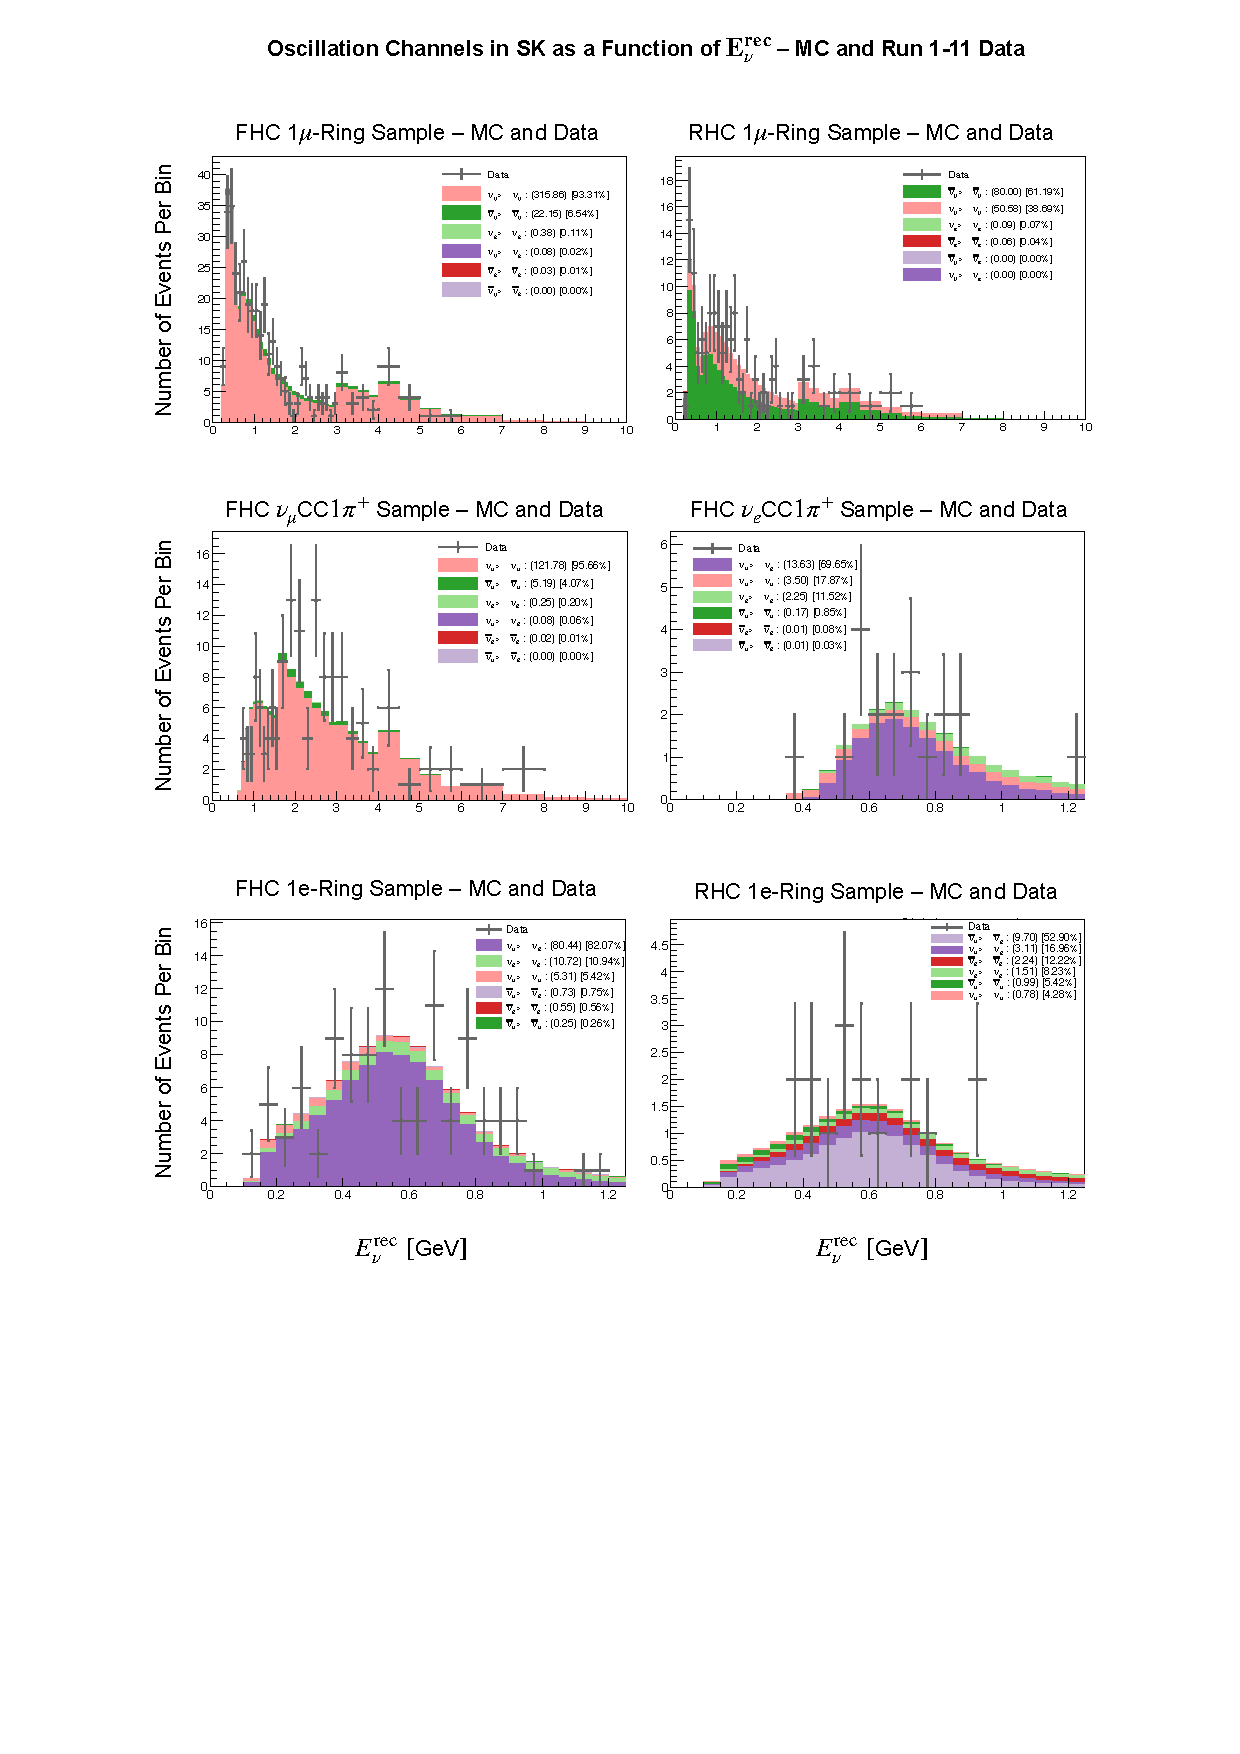
\includegraphics[width=1.\textwidth]{figures/QD_Analysis/RecoNeutrinoEnergy_ByOscChannel_Counts.pdf}
	\caption[Number of Events over $E_\nu^\mathrm{rec}$ for the Super-Kamiokande Samples (split into Oscillation Channels).]{Number of events as a function of reconstructed neutrino energy $E_\nu^\mathrm{rec}$ for the Super-Kamiokande (\acrshort{t2k} \acrshort{fd}) samples. The data from \acrshort{t2k} runs $1$ to $11$ are shown as gray dots with horizontal bars showing the bin width and vertical bars the statistical fluctuation. The \acrshort{mc} prediction is shown as a split into oscillation channels for the oscillation parameters as defined in T2K Set A ($\Gamma = 5.0 \times 10^{-15} \ \mathrm{eV}$). \Cref{fig:RecoNeutrinoEnergy_ByOscChannel_DividedByBinWidth} presents the same data normalised by bin width.}
    \label{fig:RecoNeutrinoEnergy_ByOscChannel_Counts}
    \end{figure}
%
%
    \begin{figure}[hbt]
	\centering
	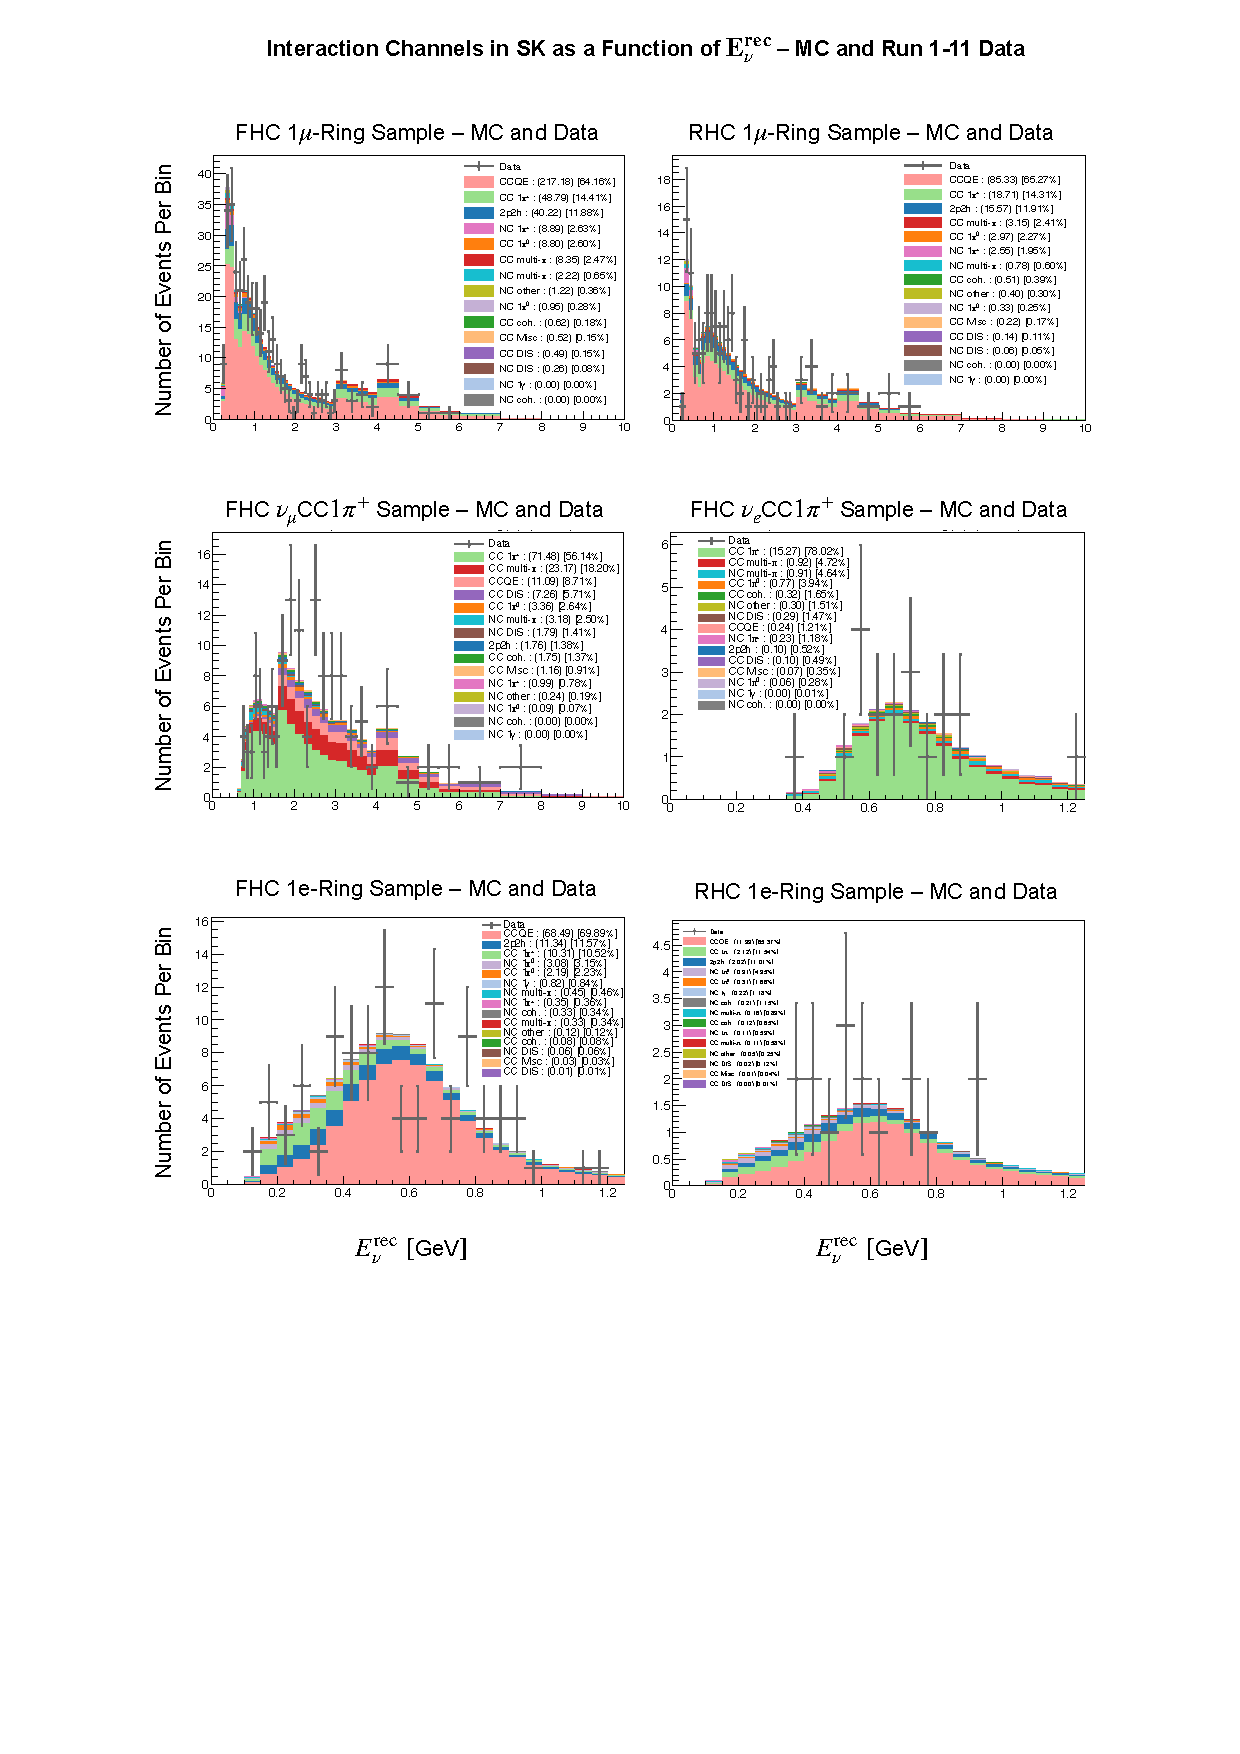
\includegraphics[width=1.\textwidth]{figures/QD_Analysis/RecoNeutrinoEnergy_ByIntChannel_Counts.pdf}
	\caption[Number of Events over $E_\nu^\mathrm{rec}$ for the Super-Kamiokande Samples (split into Interaction Channels).]{Number of events as a function of reconstructed neutrino energy $E_\nu^\mathrm{rec}$ for the Super-Kamiokande (\acrshort{t2k} \acrshort{fd}) samples. The data from \acrshort{t2k} runs $1$ to $11$ are shown as gray dots with horizontal bars showing the bin width and vertical bars the statistical fluctuation. The \acrshort{mc} prediction is broken down in interaction modes for the oscillation parameters as defined in T2K Set A ($\Gamma = 5.0 \times 10^{-15} \ \mathrm{eV}$). \Cref{fig:RecoNeutrinoEnergy_ByIntChannel_DividedByBinWidth} presents the same data normalised by bin width.}
    \label{fig:RecoNeutrinoEnergy_ByIntChannel_Counts}
    \end{figure}
%

%
\begin{figure}[hbt]
	\begin{minipage}[b]{.49\textwidth}
			$\vcenter{\hbox{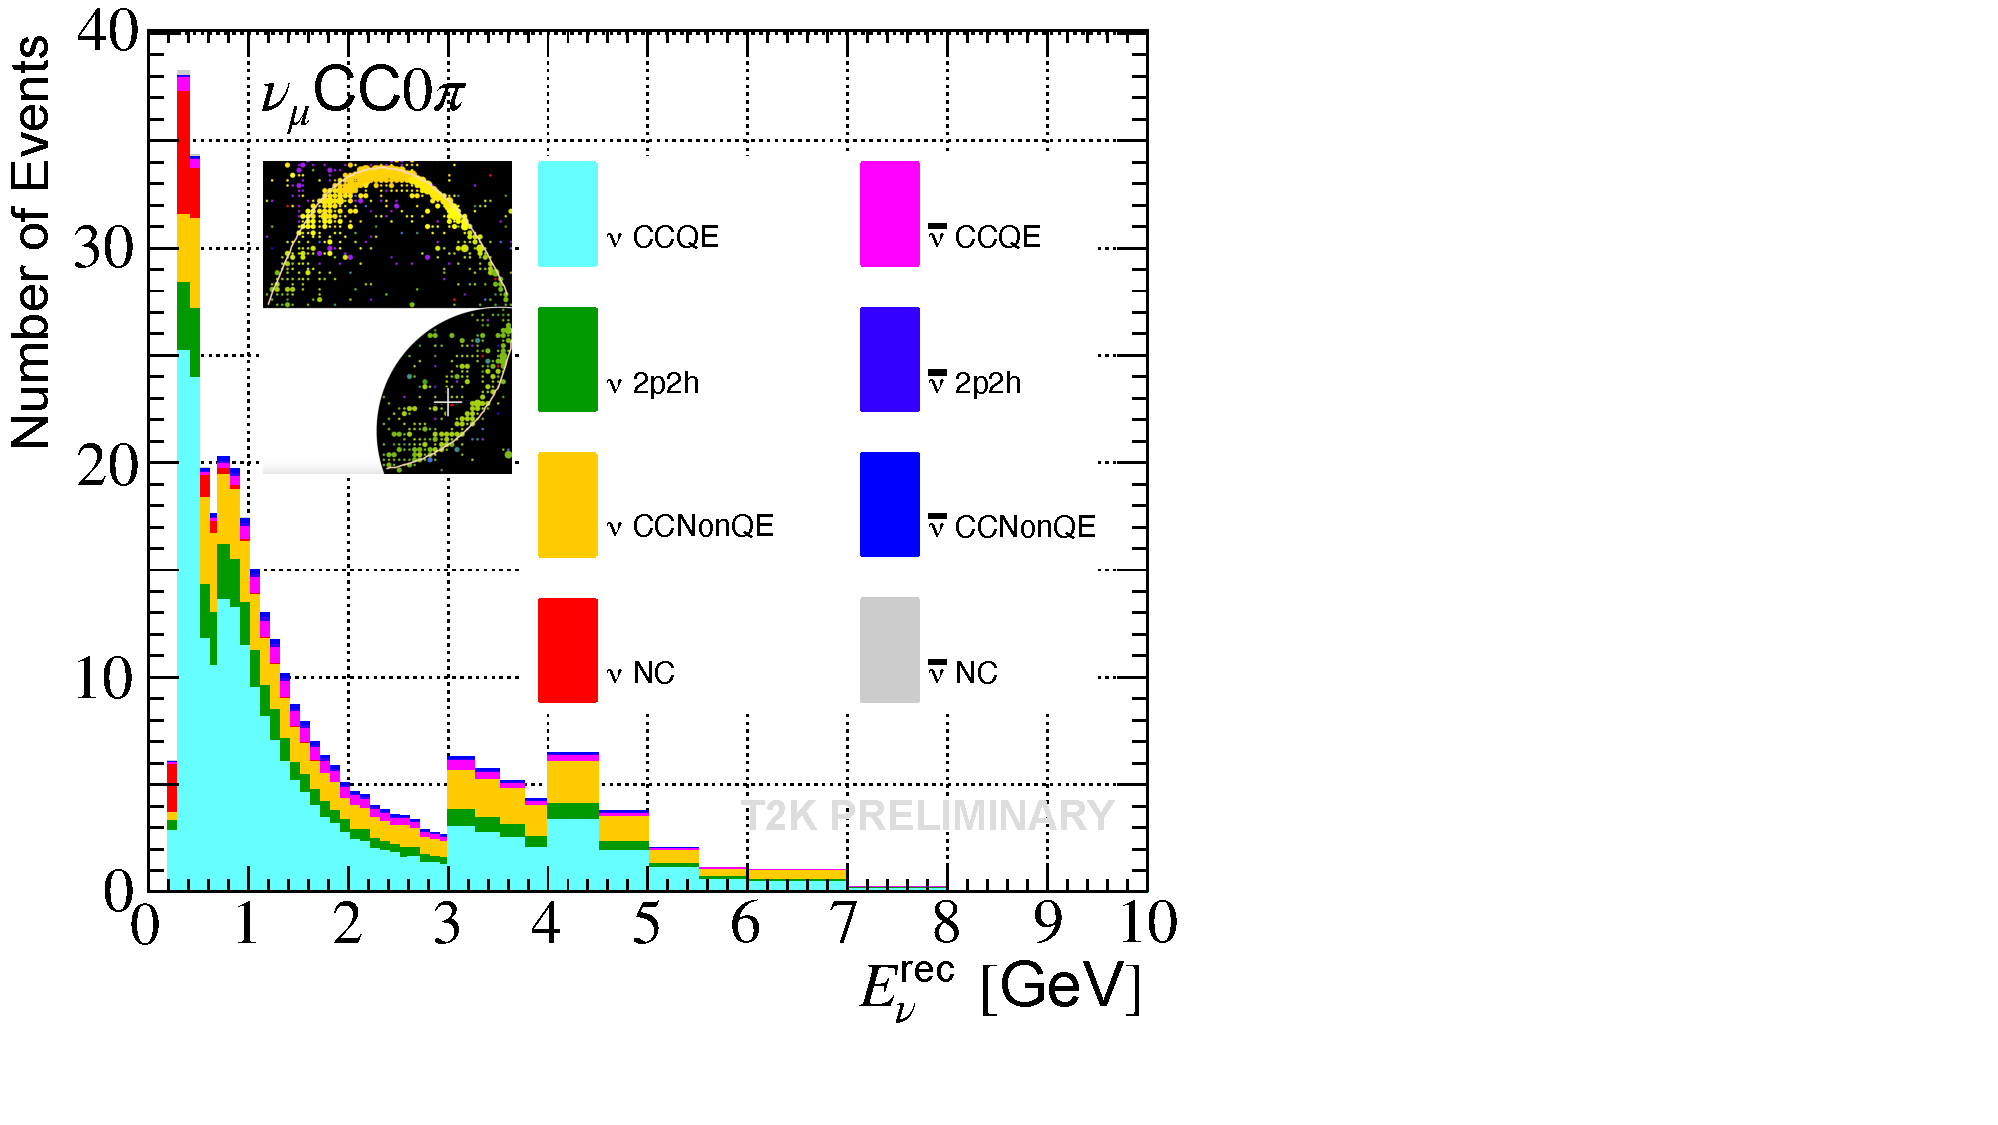
\includegraphics[width=\textwidth]
            {figures/T2K_FHC1Rmu_2024_all2}}}%{figures/T2K_FHC1Rmu_2024_all}}}%{figures/T2K_FHC1Rmu_2024_logo}}}%{figures/T2K_FHC1Rmu_2024}}}%{figures/test_t2k_outputfile_SKEventRates_Plots_ErecModeOscChanBreakdown_FHC_1Rmu_2024.pdf}}}
            $
	\end{minipage}
	\begin{minipage}[b]{.49\textwidth}
		$\vcenter{\hbox{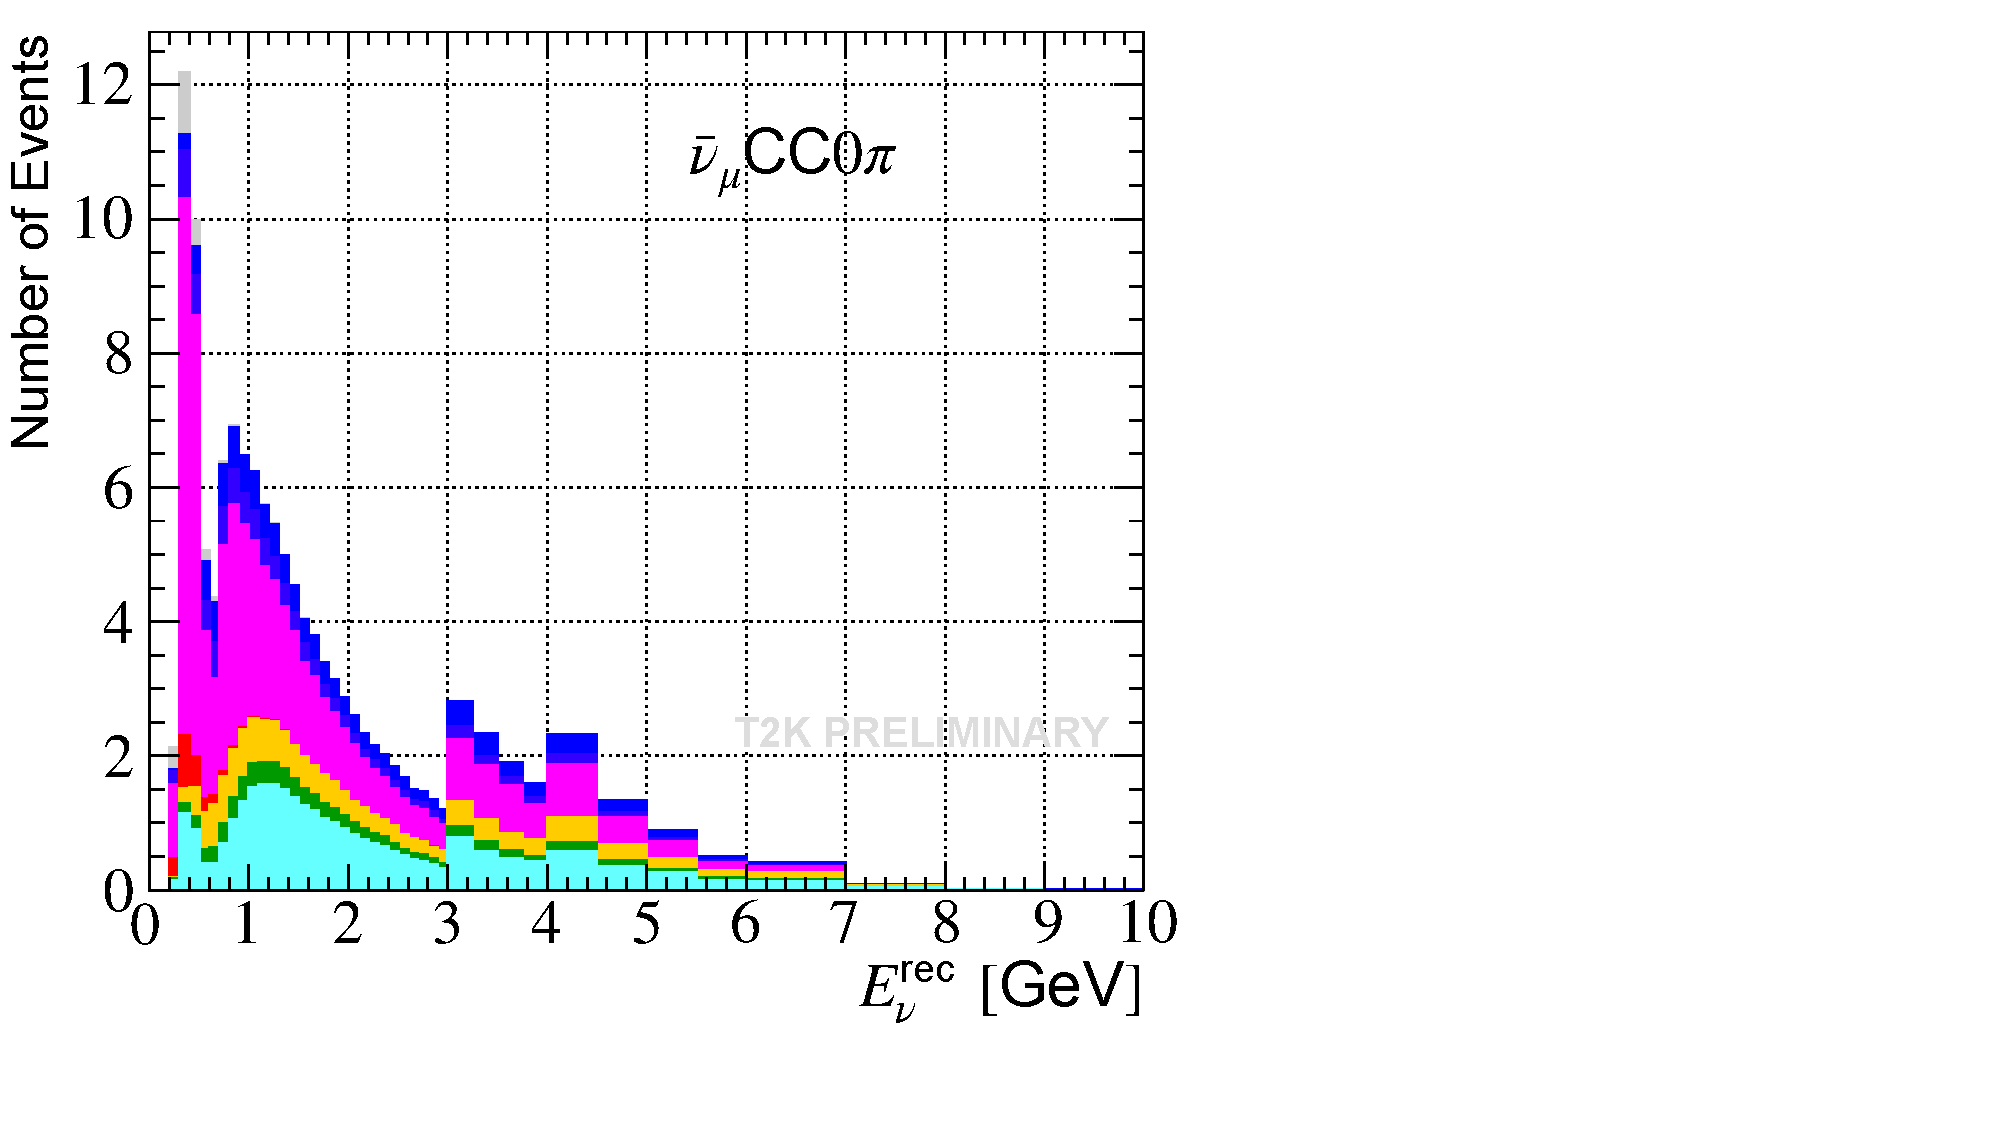
\includegraphics[width=\textwidth]
        {figures/T2K_RHC1Rmu_2024_noLogo_noLegend2.pdf}}}$
        %{figures/T2K_RHC1Rmu_2024_noLogo_noLegend.pdf}}}$
        %{figures/T2K_RHC1Rmu_2024_noLegend.pdf}}}$
        %{figures/T2K_RHC1Rmu_2024.pdf}}}$
	\end{minipage}
	\vskip\baselineskip
	\begin{minipage}[b]{.49\textwidth}
			$\vcenter{\hbox{\includegraphics[width=\textwidth]%
            {figures/T2K_FHCnumuCC1pi_20242.pdf}}}$
            %{figures/T2K_FHCnumuCC1pi_2024.pdf}}}$
	\end{minipage}
	\begin{minipage}[b]{.49\textwidth}
		$\vcenter{\hbox{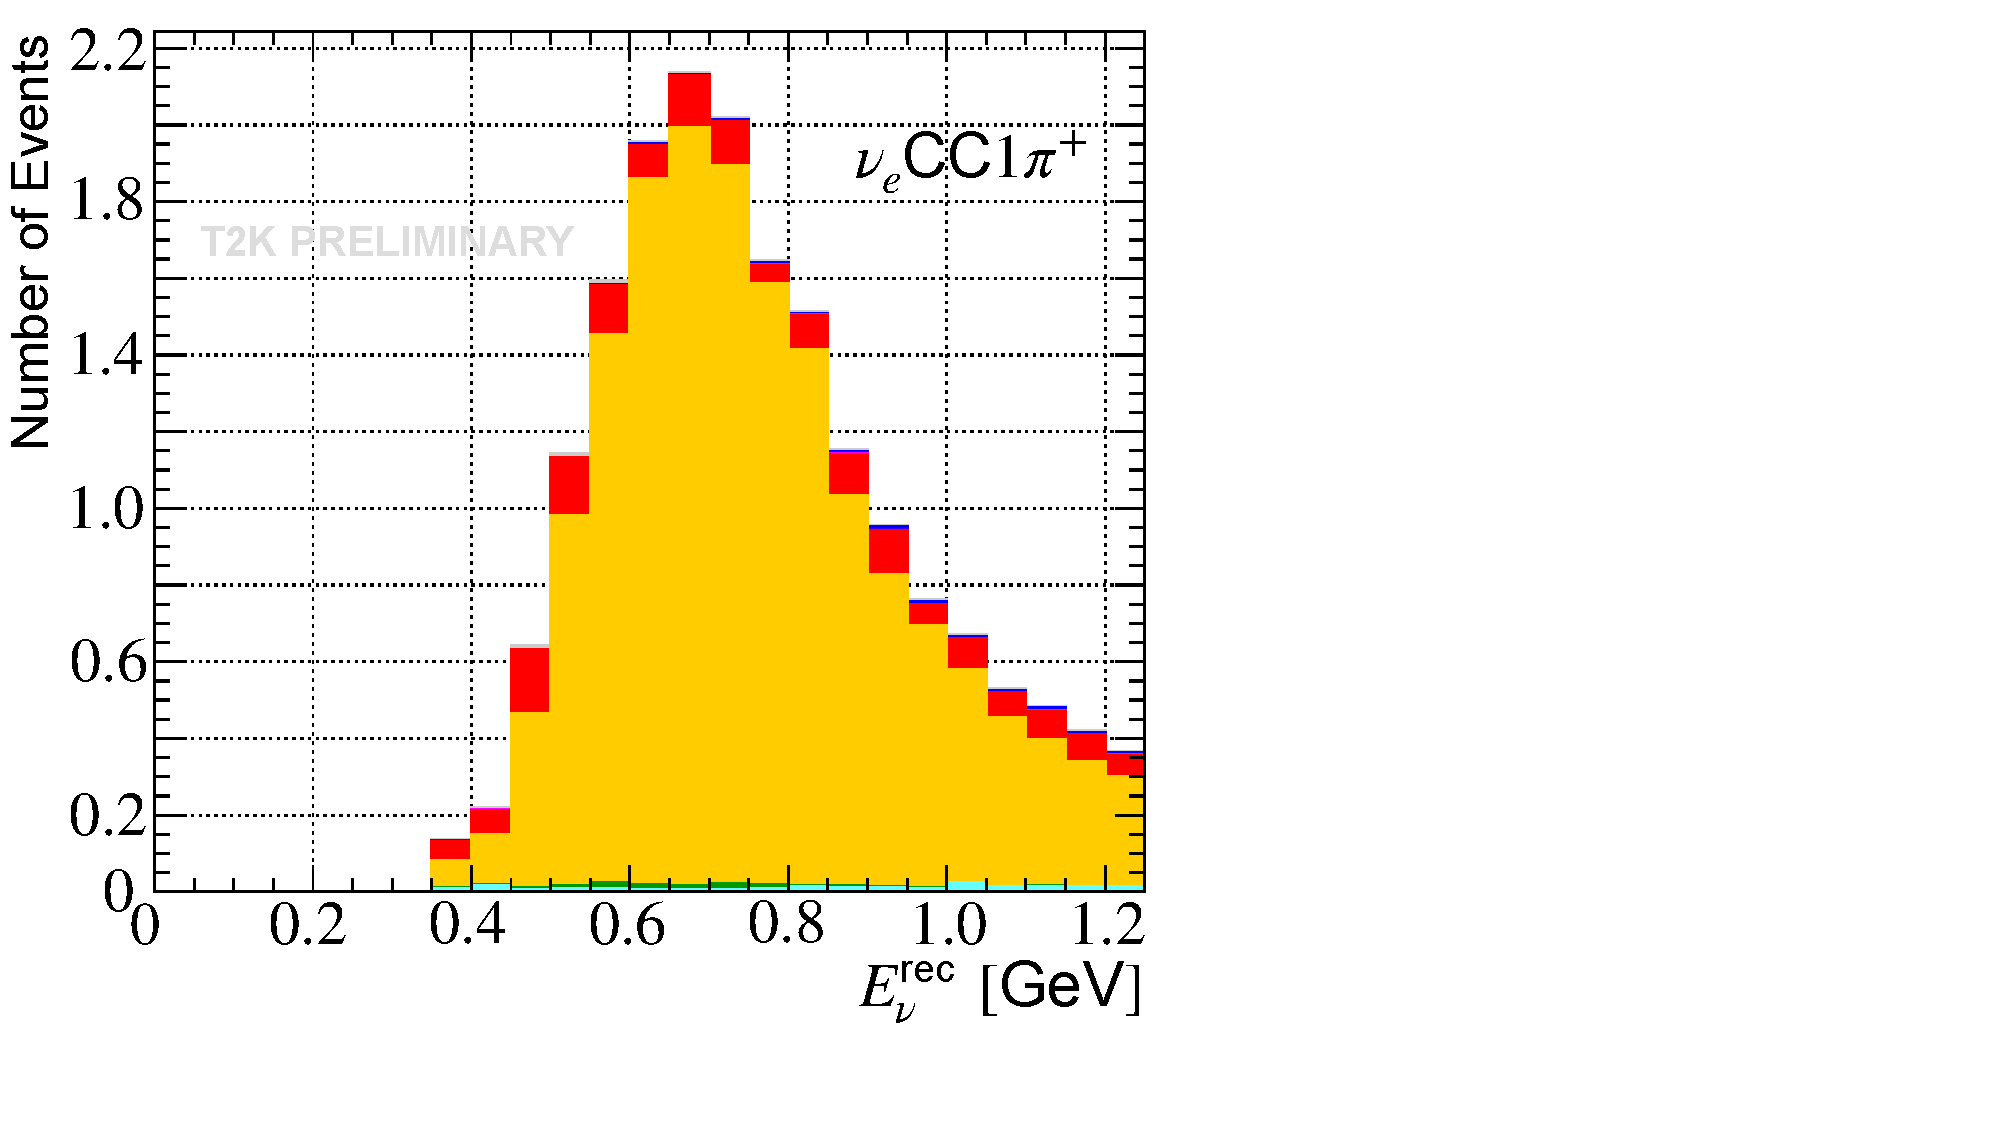
\includegraphics[width=\textwidth]
        {figures/T2K_FHCnueCC1pi_20242.pdf}}}$
        %{figures/T2K_FHCnueCC1pi_2024.pdf}}}$
	\end{minipage}
	\vskip\baselineskip
	\begin{minipage}[b]{.49\textwidth}
		$\vcenter{\hbox{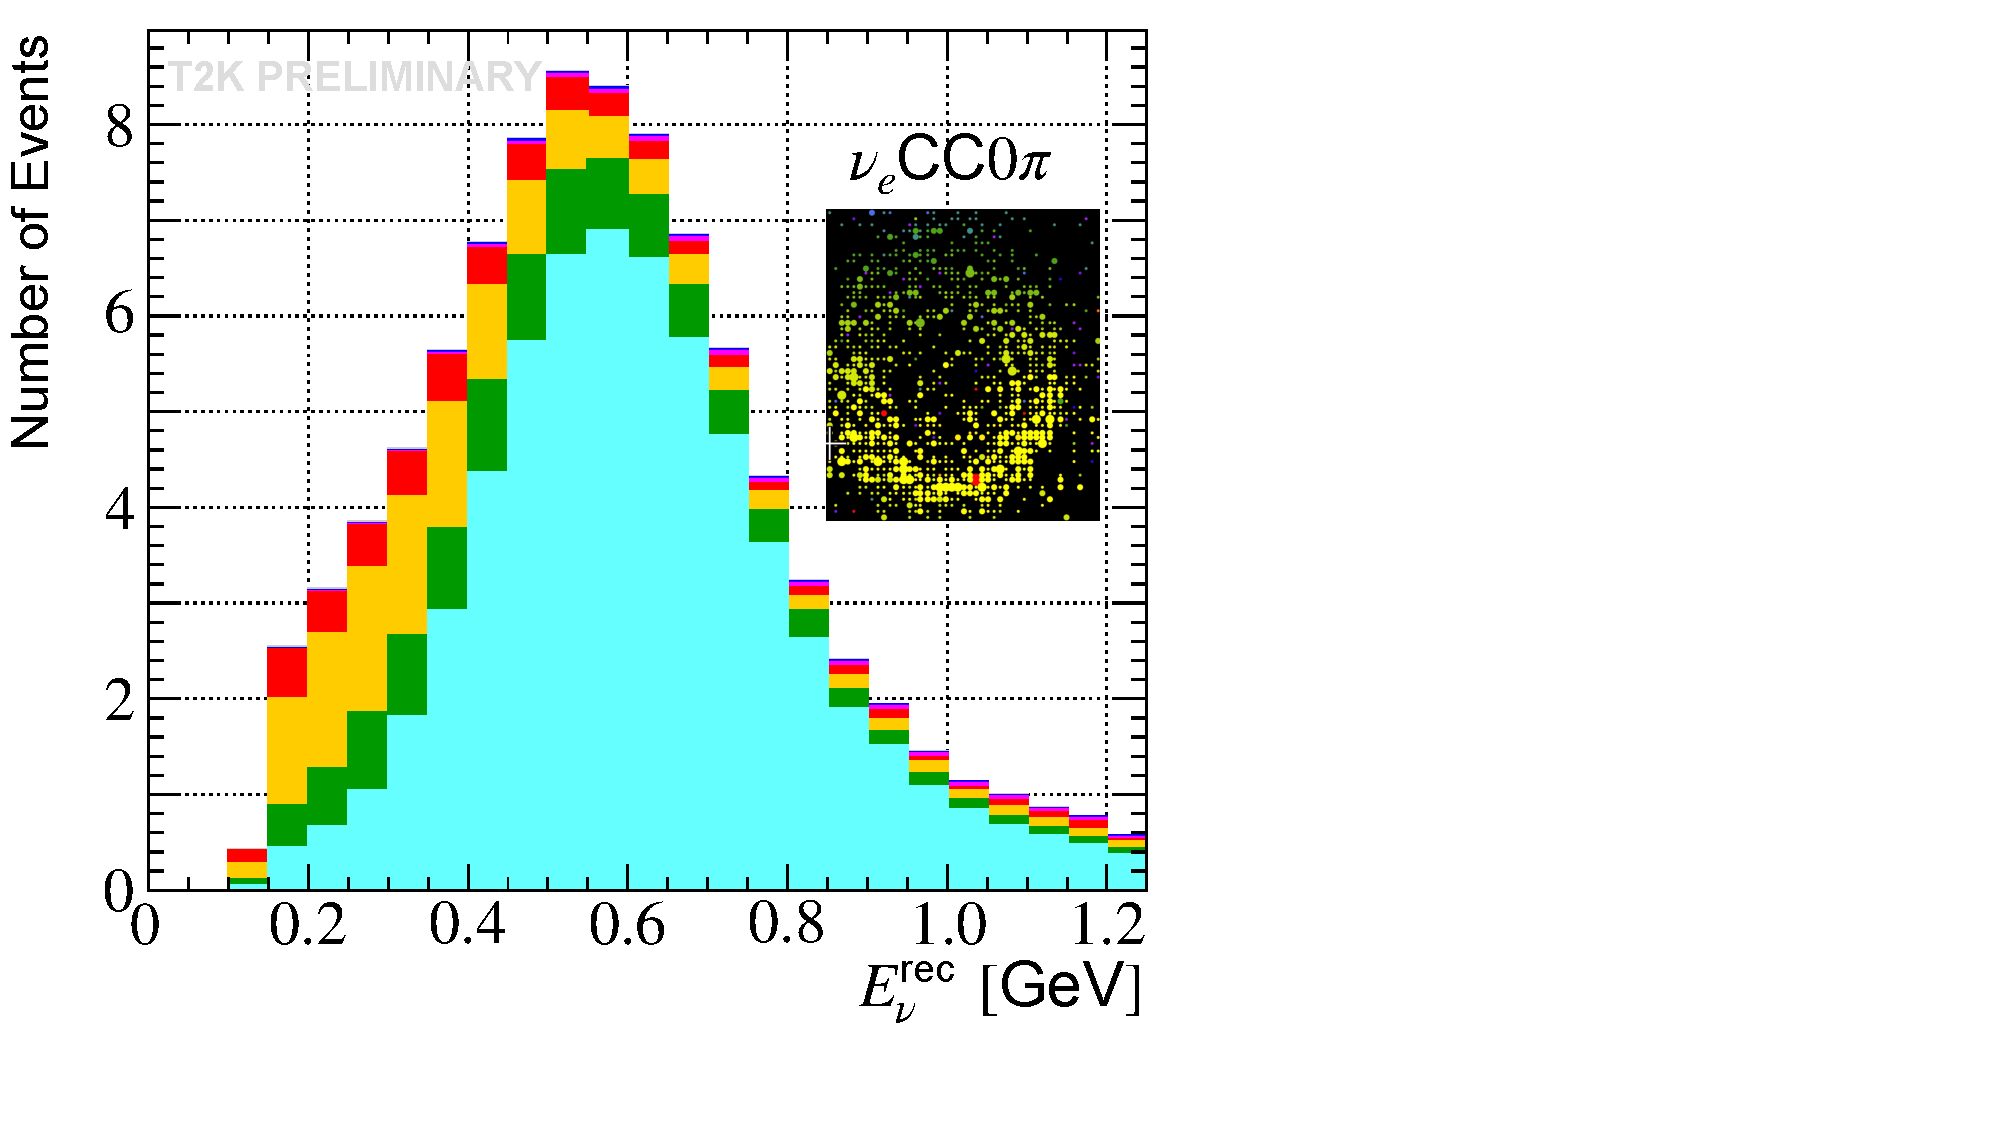
\includegraphics[width=\textwidth]
        {figures/T2K_FHC1Re_2024_all2.pdf}}}%
        %{figures/T2K_FHC1Re_2024_all.pdf}}}%{figures/T2K_FHC1Re_2024.pdf}}}%
        ]$
	\end{minipage}
	\begin{minipage}[b]{.49\textwidth}
		$\vcenter{\hbox{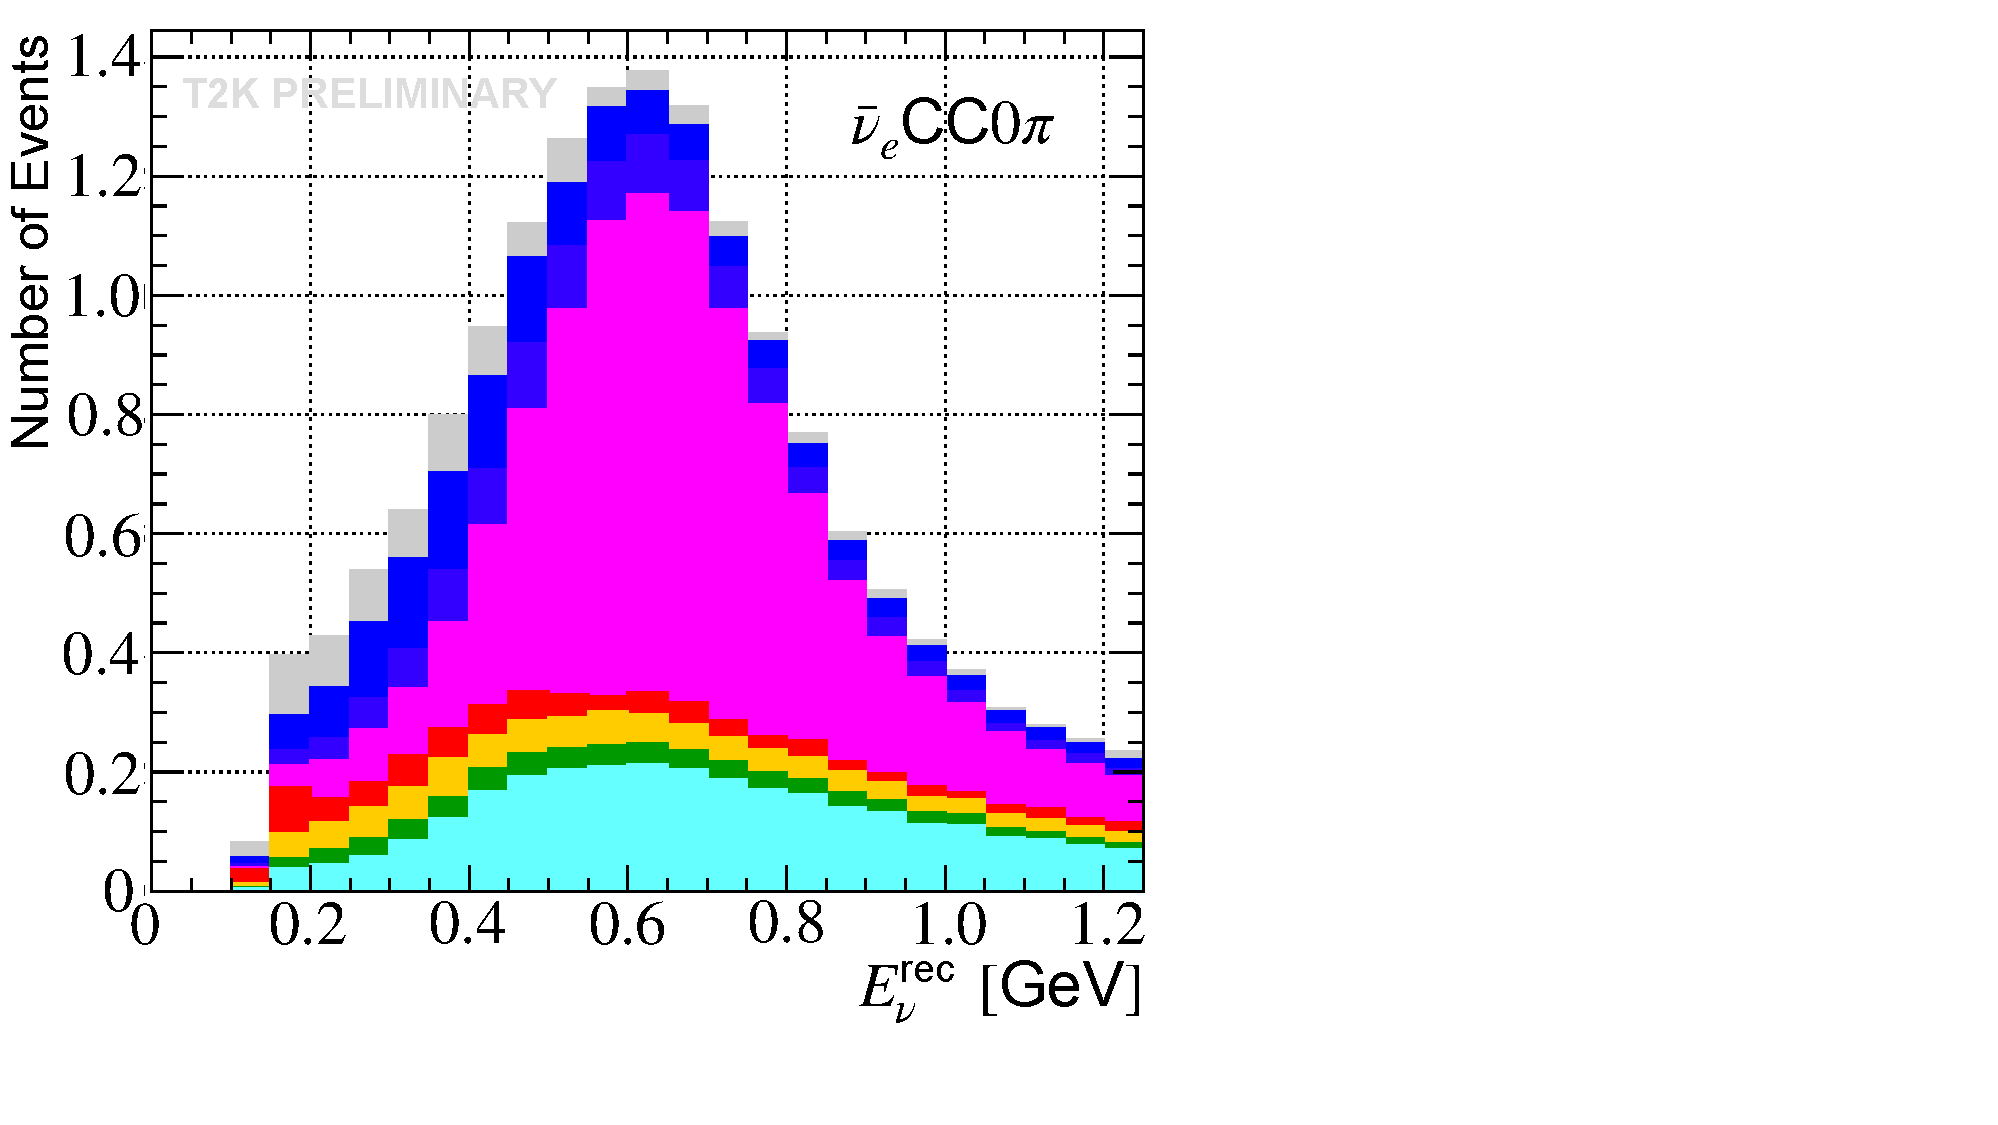
\includegraphics[width=\textwidth]
        {figures/T2K_RHC1Re_2024_noLogo2.pdf}}}$
        %{figures/T2K_RHC1Re_2024_noLogo.pdf}}}$
        %{figures/T2K_RHC1Re_2024.pdf}}}$
	\end{minipage}
	\caption[Number of Events over $E_\nu^\mathrm{rec}$ for the Super-Kamiokande Samples (split into Interaction Channels).]{Number of events as a function of reconstructed neutrino energy $E_\nu^\mathrm{rec}$ for the Super-Kamiokande (\acrshort{t2k} \acrshort{fd}) samples. The \acrshort{mc} prediction is broken down into interaction modes for the oscillation parameters as defined in T2K Set A ($\Gamma = 0.0 \ \mathrm{eV}$).} 
	\label{fig:event_spectra_t2k}
\end{figure}
%

%
    \begin{figure}[hbt]
	\centering
	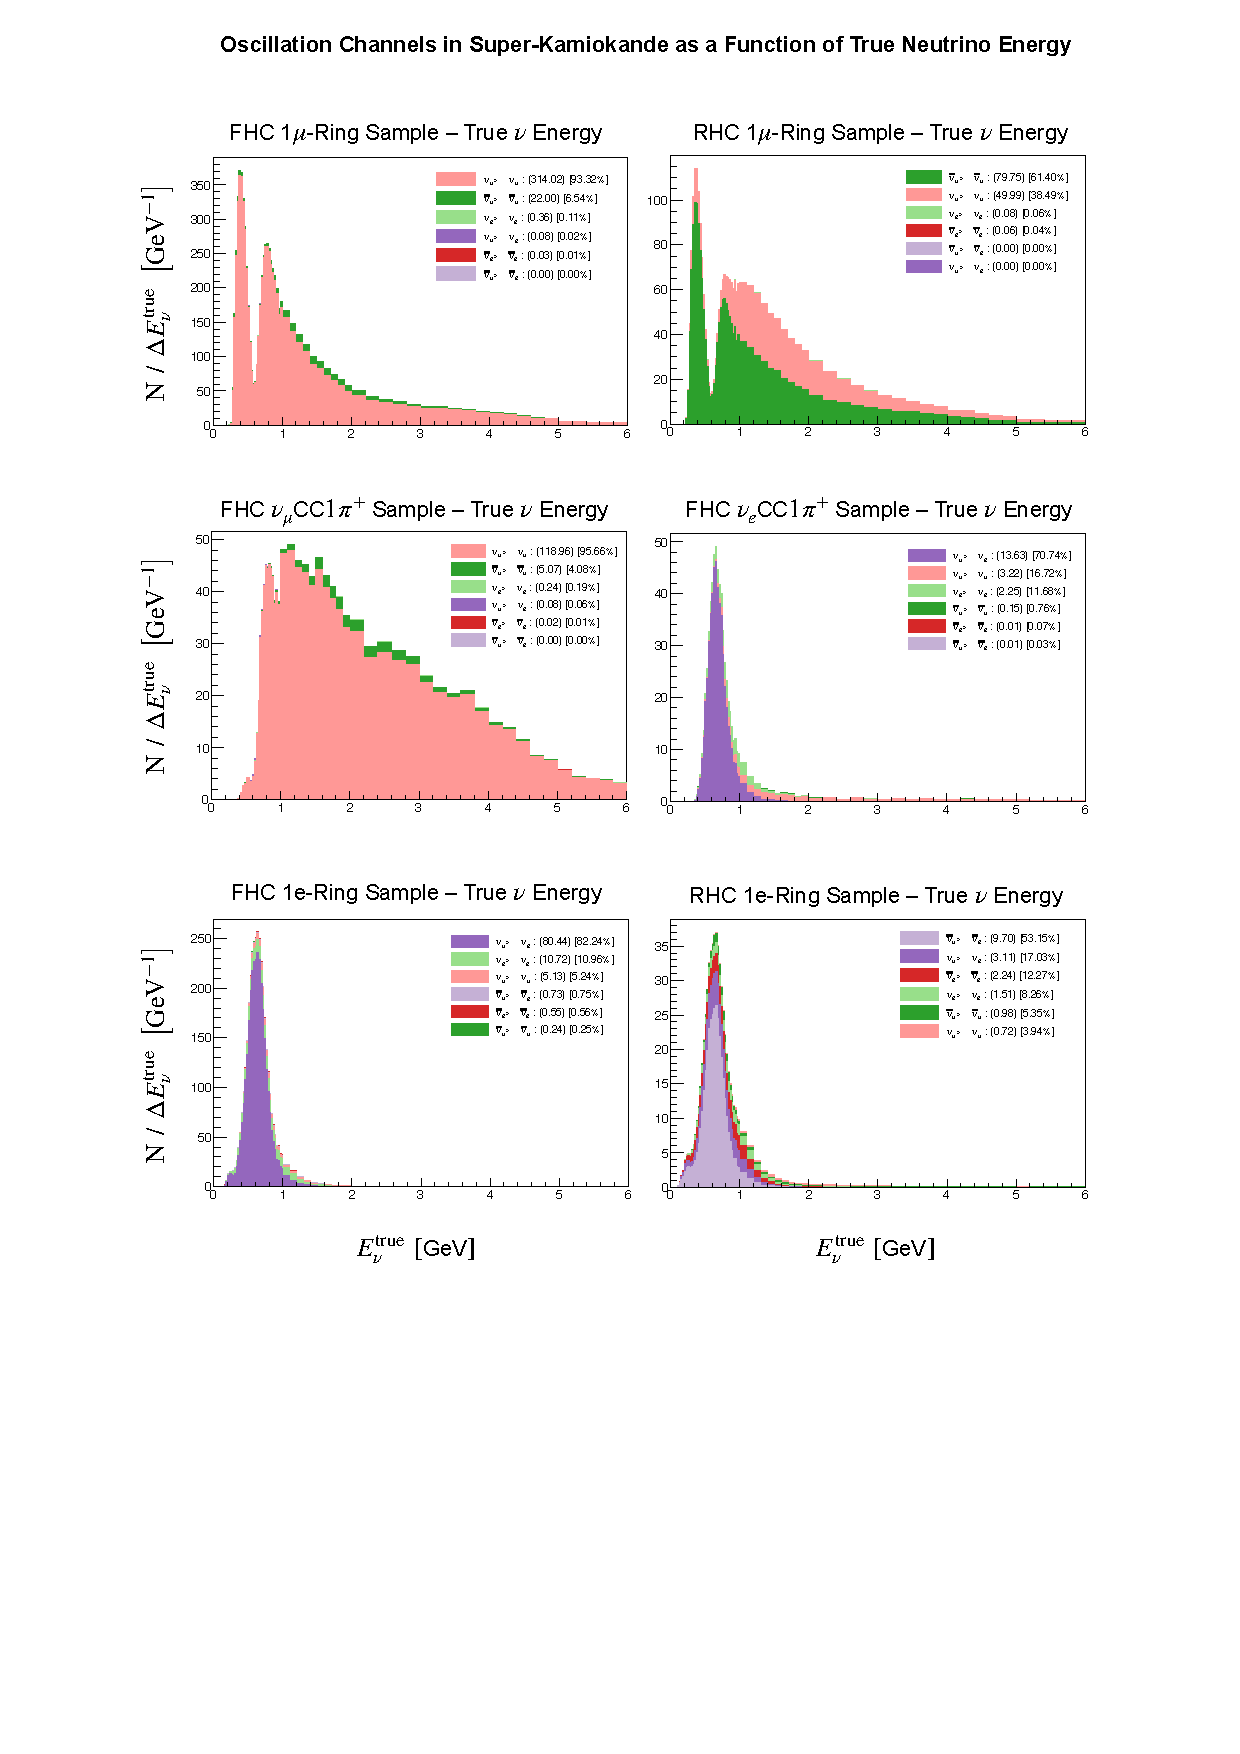
\includegraphics[width=1.\textwidth]{figures/QD_Analysis/TrueNeutrinoEnergy_ByOscChannel_DividedByBinWidth.pdf}
	\caption[Bin-Averaged Event Densities for the Super-Kamiokande Samples (split into Oscillation Channels).]{Bin-averaged event densities $N / \Delta E_\nu^\mathrm{true}$ as a function of true neutrino energy $E_\nu^\mathrm{true}$ for the Super-Kamiokande (\acrshort{t2k} \acrshort{fd})  samples. The \acrshort{mc} prediction is shown as a split into oscillation channels for the oscillation parameters as defined in T2K Set A ($\Gamma = 5.0 \times 10^{-15} \ \mathrm{eV}$). \Cref{fig:TrueNeutrinoEnergy_ByOscChannel_Counts} presents the same data undivided by bin width.}
    \label{fig:TrueNeutrinoEnergy_ByOscChannel_DividedByBinWidth}
    \end{figure}
%

%
    \begin{figure}[hbt]
	\centering
	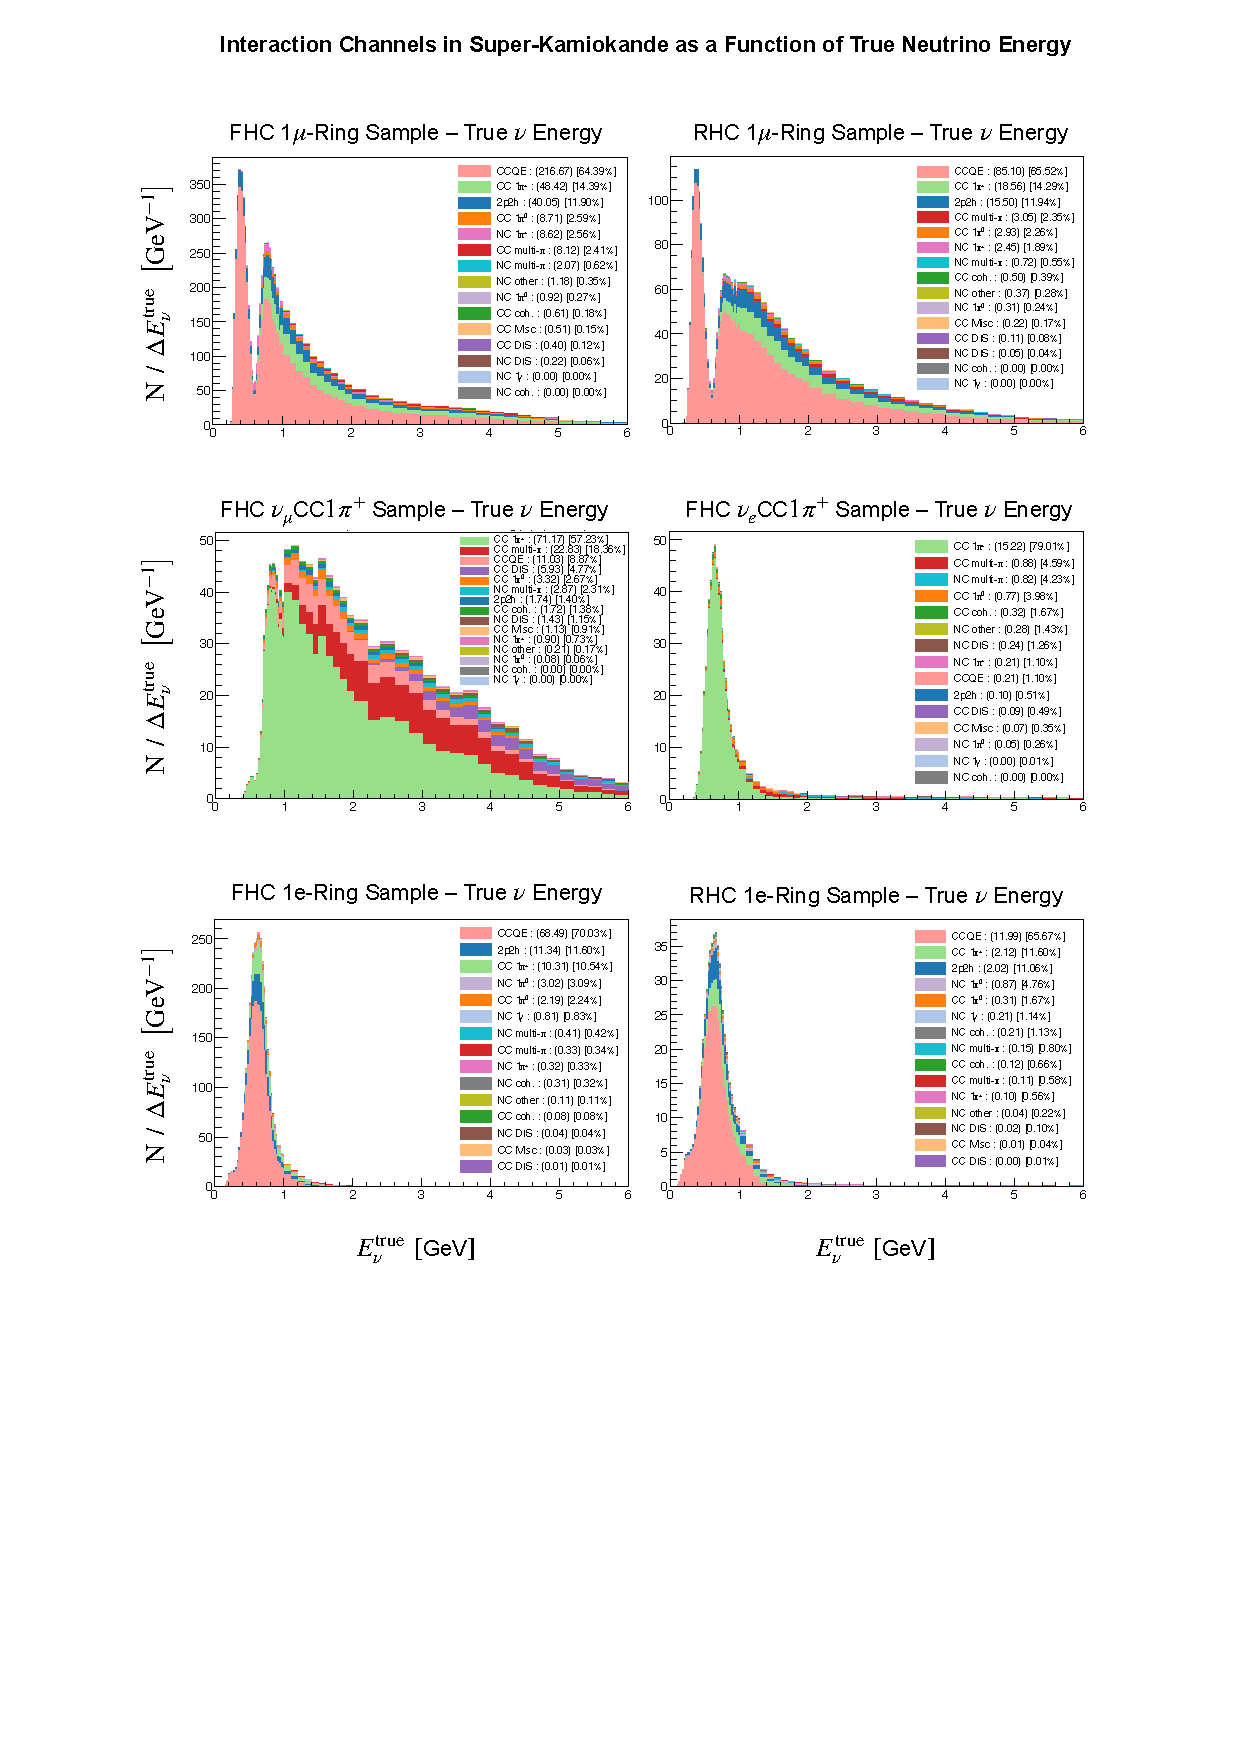
\includegraphics[width=1.\textwidth]{figures/QD_Analysis/TrueNeutrinoEnergy_ByIntChannel_DividedByBinWidth.pdf}
	\caption[Bin-Averaged Event Densities over $E_\nu^\mathrm{true}$ for the Super-Kamiokande Samples (split into Interaction Channels).]{Bin-averaged event densities $N / \Delta E_\nu^\mathrm{true}$ as a function of true neutrino energy $E_\nu^\mathrm{true}$ for the Super-Kamiokande (\acrshort{t2k} \acrshort{fd}) samples. The \acrshort{mc} prediction is broken down into interaction modes for the oscillation parameters as defined in T2K Set A ($\Gamma = 5.0 \times 10^{-15} \ \mathrm{eV}$). \Cref{fig:TrueNeutrinoEnergy_ByIntChannel_Counts} presents the same data undivided by bin width.}
    \label{fig:TrueNeutrinoEnergy_ByIntChannel_DividedByBinWidth}
    \end{figure}
%

%
    \begin{figure}[hbt]
	\centering
	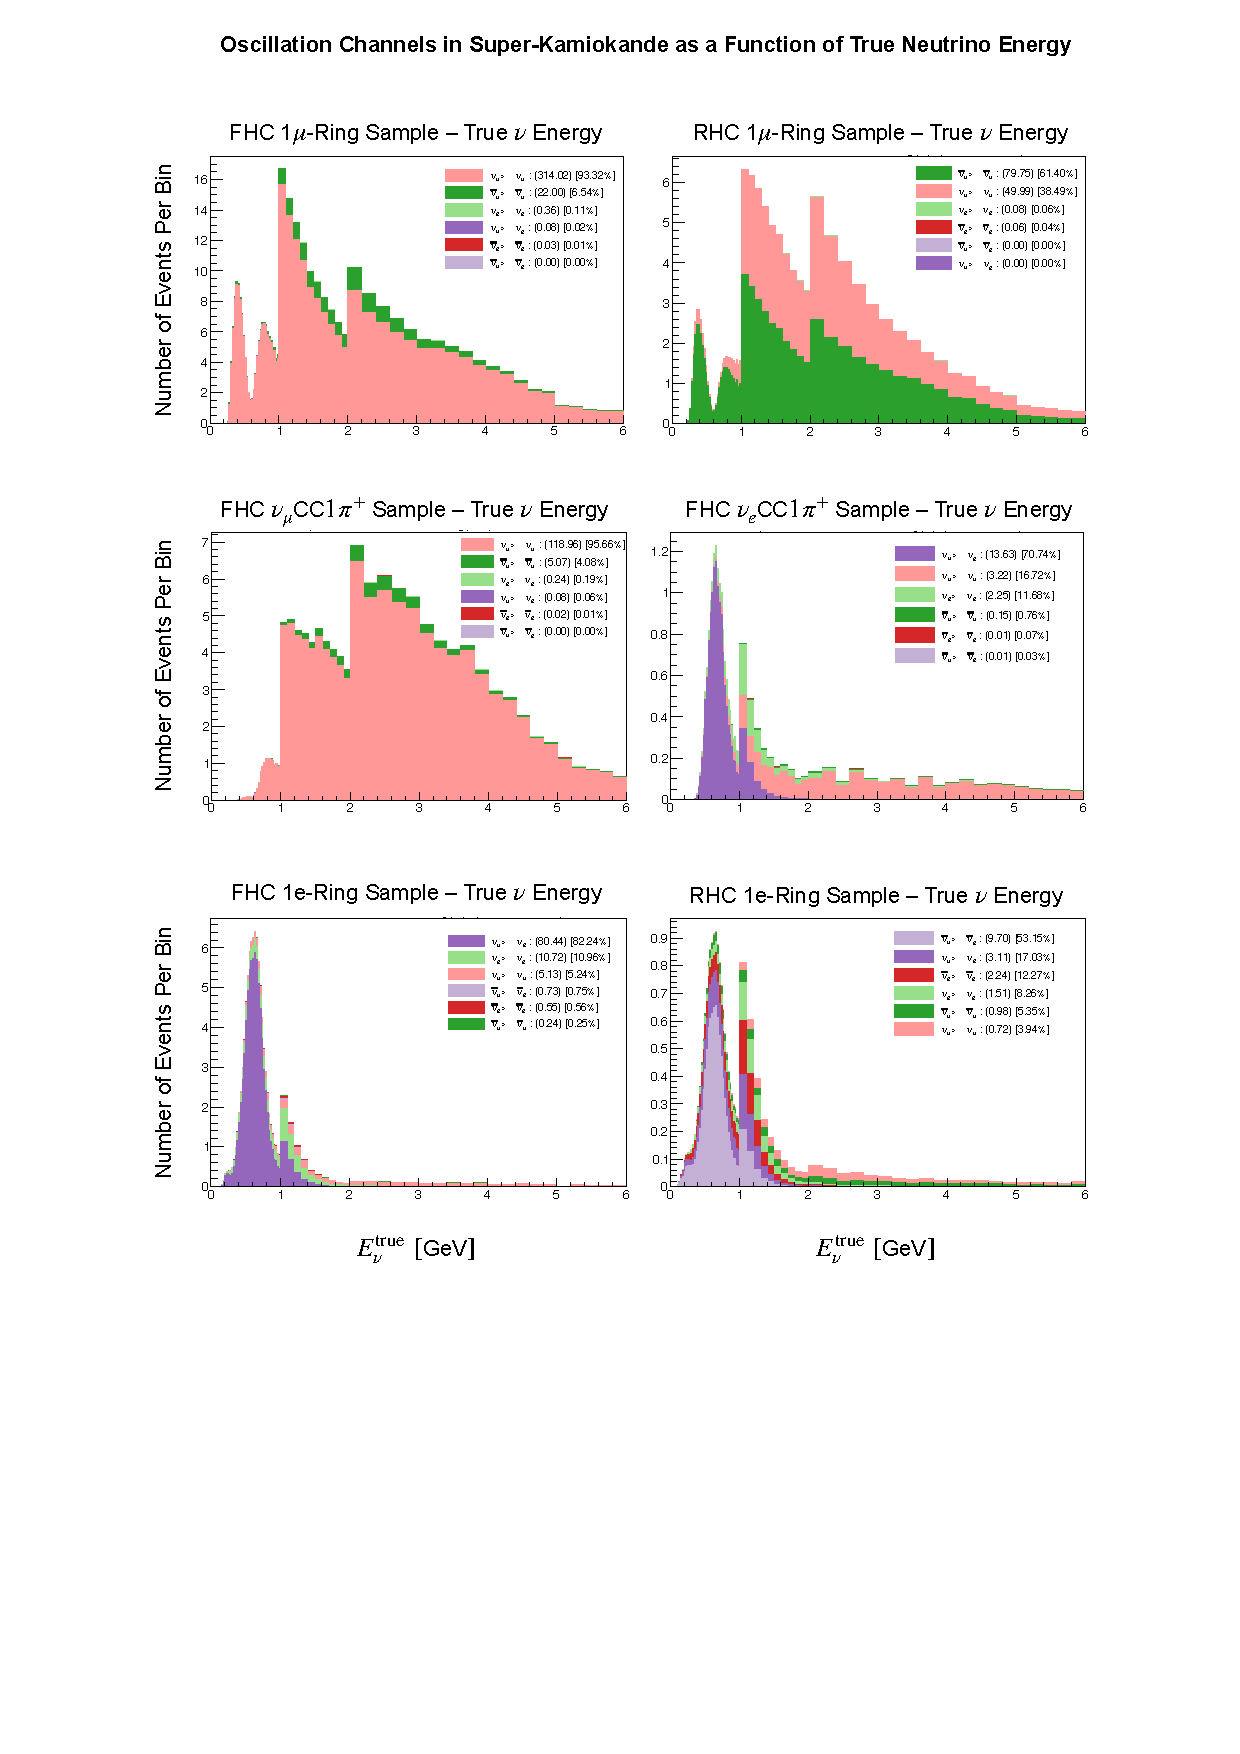
\includegraphics[width=1.\textwidth]{figures/QD_Analysis/TrueNeutrinoEnergy_ByOscChannel_Counts.pdf}
	\caption[Number of Events over $E_\nu^\mathrm{true}$ for the Super-Kamiokande Samples (split into Oscillation Channels).]{Number of events as a function of reconstructed neutrino energy $E_\nu^\mathrm{true}$ for the Super-Kamiokande (\acrshort{t2k} \acrshort{fd}) samples. The \acrshort{mc} prediction is shown as a split into oscillation channels for the oscillation parameters as defined in T2K Set A ($\Gamma = 5.0 \times 10^{-15} \ \mathrm{eV}$). \Cref{fig:TrueNeutrinoEnergy_ByOscChannel_DividedByBinWidth} presents the same data normalised by bin width.}
    \label{fig:TrueNeutrinoEnergy_ByOscChannel_Counts}
    \end{figure}
%

%
    \begin{figure}[hbt]
	\centering
	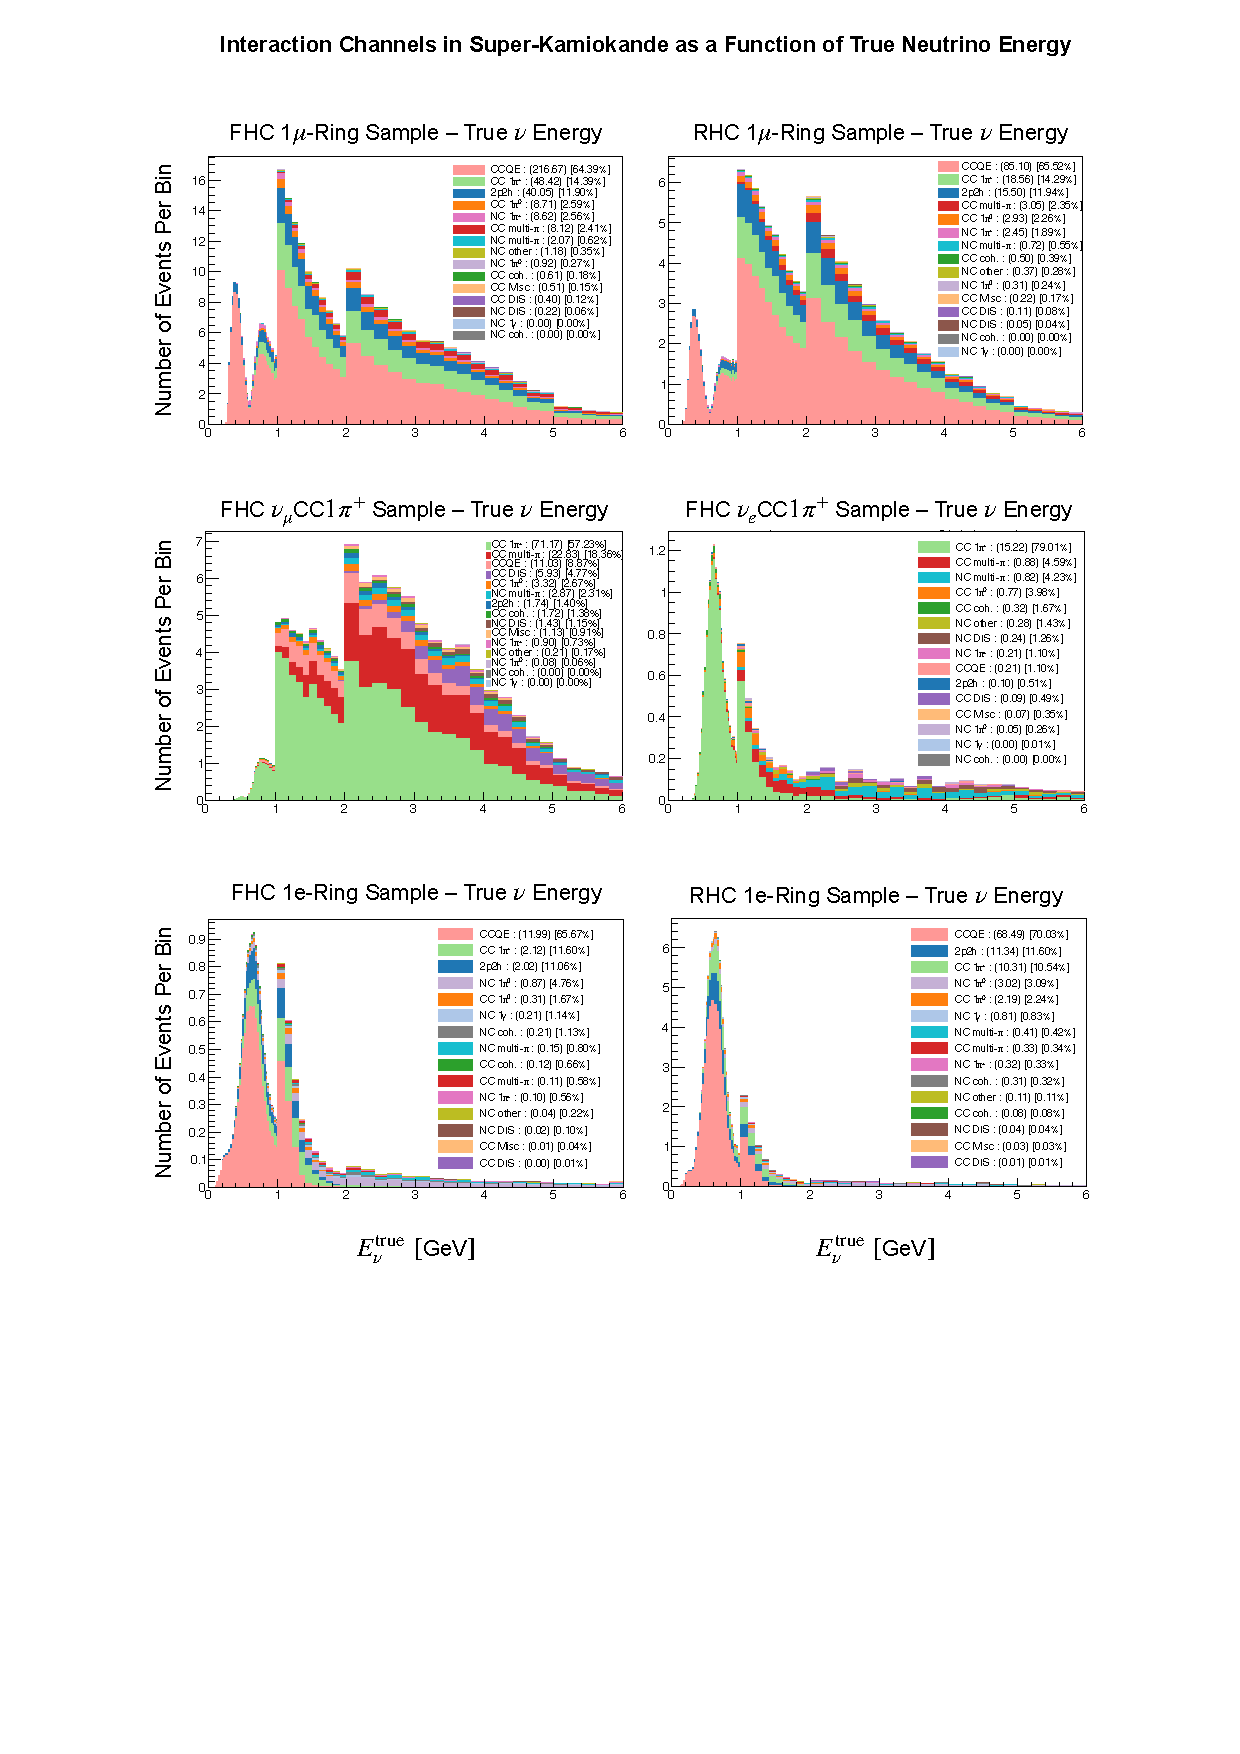
\includegraphics[width=1.\textwidth]{figures/QD_Analysis/TrueNeutrinoEnergy_ByIntChannel_Counts.pdf}
	\caption[Number of Events over $E_\nu^\mathrm{true}$ for the Super-Kamiokande Samples (split into Interaction Channels).]{Number of events as a function of reconstructed neutrino energy $E_\nu^\mathrm{true}$ for the Super-Kamiokande (\acrshort{t2k} \acrshort{fd}) samples. The \acrshort{mc} prediction is broken down into interaction modes for the oscillation parameters as defined in T2K Set A ($\Gamma = 5.0 \times 10^{-15} \ \mathrm{eV}$). \Cref{fig:TrueNeutrinoEnergy_ByIntChannel_DividedByBinWidth} presents the same data normalised by bin width.}
    \label{fig:TrueNeutrinoEnergy_ByIntChannel_Counts}
    \end{figure}
%

\newpage

%
%\begin{landscape}
\begin{table}[H]
\caption[]{Upper limits (U) and Sensitivities (S) on the quantum decoherence strength $\Gamma_0$ [eV] for different choices for the energy scale $n$. Reference energy $E_0=1$ GeV.}
\label{tab:params_settings1}
\resizebox{\textwidth}{!}{%
\begin{tabular}{|l|l|l||c|c|c|c|c|c|c|}
    \hline
    \textbf{Model} & \textbf{Experiment} & \textbf{Ref.}
        & $n=-3$ & $n=-2$ & $n=-1$ & $n=0$ & $n=1$ & $n=2$ & $n=3$ \\ \hline \hline

\multirow{13}{*}{\parbox{3.2cm}{\centering 
Phase Perturbation \\[0.5ex]
\scriptsize $\mathrm{diag}(0,\Gamma,\Gamma,0,\Gamma,\Gamma,\Gamma,\Gamma,0)$}}
        & ANTARES          & ... & ... & ... & ... & ... & ... & ... & ... \\ \cline{2-10}
        & Borexino         & ... & ... & ... & ... & ... & ... & ... & ... \\ \cline{2-10}
        & Daya Bay (U)        & ... & ... & ... & ... & ... & ... & ... & ... \\ \cline{2-10}
        & DUNE (S)            & ... & ... & ... & ... & ... & ... & ... & ... \\ \cline{2-10}
        & HK (S)              & ... & ... & ... & ... & ... & ... & ... & ... \\ \cline{2-10}
        & IceCube (U)         & \cite{ICECUBE:2023gdv} & ... & ... & ... & $1.18\times 10^{-15}$ & $6.89\times 10^{-19}$ & $9.80\times 10^{-24}$ & $1.58\times 10^{-28}$ \\ \cline{2-10}
        & JUNO (S)            & ... & ... & ... & ... & ... & ... & ... & ... \\ \cline{2-10}
        & KamLAND (U)         & ... & ... & ... & ... & ... & ... & ... & ... \\ \cline{2-10}
        & Km3NET (U)          & ... & ... & ... & ... & ... & ... & ... & ... \\ \cline{2-10}
        & MINOS (U)           & ... & ... & ... & ... & ... & ... & ... & ... \\ \cline{2-10}
        & NOvA (U)            & ... & ... & ... & ... & ... & ... & ... & ... \\ \cline{2-10}
        & RENO (U)            & ... & ... & ... & ... & ... & ... & ... & ... \\ \cline{2-10}
        & SK (U)             & ... & ... & ... & ... & ... & ... & ... & ... \\ \cline{2-10}
        & T2K (U)            & \cite{DeRomeri:2023dht} & ... & $1.00\times 10^{-14}$ & $3.00\times 10^{-14}$ & $5.00\times 10^{-14}$ & $7.00\times 10^{-14}$ & $9.00\times 10^{-14}$ & ... \\ \hline \hline


\multirow{13}{*}{\parbox{3.2cm}{\centering 
State Selected \\[0.5ex]
\scriptsize $\mathrm{diag}(0,\Gamma,\Gamma,\Gamma,\Gamma,\Gamma,\Gamma,\Gamma,\Gamma)$}}
        & ANTARES          & ... & ... & ... & ... & ... & ... & ... & ... \\ \cline{2-10}
        & Borexino         & ... & ... & ... & ... & ... & ... & ... & ... \\ \cline{2-10}
        & Daya Bay         & ... & ... & ... & ... & ... & ... & ... & ... \\ \cline{2-10}
        & DUNE             & ... & ... & ... & ... & ... & ... & ... & ... \\ \cline{2-10}
        & HK & ... & ... & ... & ... & ... & ... & ... & ... \\ \cline{2-10}
        & IceCube          & ... & ... & ... & ... & ... & ... & ... & ... \\ \cline{2-10}
        & JUNO             & ... & ... & ... & ... & ... & ... & ... & ... \\ \cline{2-10}
        & KamLAND          & ... & ... & ... & ... & ... & ... & ... & ... \\ \cline{2-10}
        & Km3NET           & ... & ... & ... & ... & ... & ... & ... & ... \\ \cline{2-10}
        & MINOS            & ... & ... & ... & ... & ... & ... & ... & ... \\ \cline{2-10}
        & NOvA             & ... & ... & ... & ... & ... & ... & ... & ... \\ \cline{2-10}
        & RENO             & ... & ... & ... & ... & ... & ... & ... & ... \\ \cline{2-10}
        & SK               & ... & ... & ... & ... & ... & ... & ... & ... \\ \cline{2-10}
        & T2K              & ... & ... & ... & ... & ... & ... & ... & ... \\ \hline \hline


\multirow{13}{*}{\parbox{3.2cm}{\centering 
Neutrino Loss \\[0.5ex]
\scriptsize $\mathrm{diag}(\Gamma,\Gamma,\Gamma,\Gamma,\Gamma,\Gamma,\Gamma,\Gamma,\Gamma)$}}
        & ANTARES          & ... & ... & ... & ... & ... & ... & ... & ... \\ \cline{2-10}
        & Borexino         & ... & ... & ... & ... & ... & ... & ... & ... \\ \cline{2-10}
        & Daya Bay         & ... & ... & ... & ... & ... & ... & ... & ... \\ \cline{2-10}
        & DUNE             & ... & ... & ... & ... & ... & ... & ... & ... \\ \cline{2-10}
        & HK & ... & ... & ... & ... & ... & ... & ... & ... \\ \cline{2-10}
        & IceCube          & ... & ... & ... & ... & ... & ... & ... & ... \\ \cline{2-10}
        & JUNO             & ... & ... & ... & ... & ... & ... & ... & ... \\ \cline{2-10}
        & KamLAND          & ... & ... & ... & ... & ... & ... & ... & ... \\ \cline{2-10}
        & Km3NET           & ... & ... & ... & ... & ... & ... & ... & ... \\ \cline{2-10}
        & MINOS            & ... & ... & ... & ... & ... & ... & ... & ... \\ \cline{2-10}
        & NOvA             & ... & ... & ... & ... & ... & ... & ... & ... \\ \cline{2-10}
        & RENO             & ... & ... & ... & ... & ... & ... & ... & ... \\ \cline{2-10}
        & SK               & ... & ... & ... & ... & ... & ... & ... & ... \\ \cline{2-10}
        & T2K              & ... & ... & ... & ... & ... & ... & ... & ... \\ \hline \hline


\multirow{3}{*}{\parbox{3.2cm}{\centering 
Model B \\[0.5ex]
\scriptsize $\mathrm{diag}(0, \Gamma, \Gamma, 0, \Gamma, \Gamma, 0, 0, 0)$}}
        & ANTARES          & ... & ... & ... & ... & ... & ... & ... & ... \\ \cline{2-10}
        & Borexino         & ... & ... & ... & ... & ... & ... & ... & ... \\ \cline{2-10}
        & Daya Bay         & ... & ... & ... & ... & ... & ... & ... & ... \\ \cline{2-10}
        & DUNE             & ... & ... & ... & ... & ... & ... & ... & ... \\ \cline{2-10}
        & HK               & ... & ... & ... & ... & ... & ... & ... & ... \\ \cline{2-10}
        & IceCube          & ... & ... & ... & ... & ... & ... & ... & ... \\ \cline{2-10}
        & JUNO             & ... & ... & ... & ... & ... & ... & ... & ... \\ \cline{2-10}
        & KamLAND          & ... & ... & ... & ... & ... & ... & ... & ... \\ \cline{2-10}
        & Km3NET           & ... & ... & ... & ... & ... & ... & ... & ... \\ \cline{2-10}
        & MINOS            & ... & ... & ... & ... & ... & ... & ... & ... \\ \cline{2-10}
        & NOvA             & ... & ... & ... & ... & ... & ... & ... & ... \\ \cline{2-10}
        & RENO             & ... & ... & ... & ... & ... & ... & ... & ... \\ \cline{2-10}
        & SK               & ... & ... & ... & ... & ... & ... & ... & ... \\ \cline{2-10}
        & T2K              & ... & ... & ... & ... & ... & ... & ... & ... \\ \hline \hline
\end{tabular}
} % end resizebox
\end{table}

\begin{table}[H]
\caption[]{Upper limits (U) and Sensitivities (S) on the quantum decoherence strength $\Gamma_0$ [eV] for different choices for the energy scale $n$. Reference energy $E_0=1$ GeV.}
\label{tab:params_settings2}
\resizebox{\textwidth}{!}{%
\begin{tabular}{|l|l|l||c|c|c|c|c|c|c|}
    \hline
    \textbf{Model} & \textbf{Experiment} & \textbf{Ref.}
        & $n=-3$ & $n=-2$ & $n=-1$ & $n=0$ & $n=1$ & $n=2$ & $n=3$ \\ \hline \hline
        
\multirow{3}{*}{\parbox{3.2cm}{\centering 
Model C \\[0.5ex]
\scriptsize $\mathrm{diag}(0, \Gamma, \Gamma, 0, 0, 0, \Gamma, \Gamma, 0)$}}
        & ANTARES          & ... & ... & ... & ... & ... & ... & ... & ... \\ \cline{2-10}
        & Borexino         & ... & ... & ... & ... & ... & ... & ... & ... \\ \cline{2-10}
        & Daya Bay         & ... & ... & ... & ... & ... & ... & ... & ... \\ \cline{2-10}
        & DUNE             & ... & ... & ... & ... & ... & ... & ... & ... \\ \cline{2-10}
        & HK & ... & ... & ... & ... & ... & ... & ... & ... \\ \cline{2-10}
        & IceCube          & ... & ... & ... & ... & ... & ... & ... & ... \\ \cline{2-10}
        & JUNO             & ... & ... & ... & ... & ... & ... & ... & ... \\ \cline{2-10}
        & KamLAND          & ... & ... & ... & ... & ... & ... & ... & ... \\ \cline{2-10}
        & Km3NET           & ... & ... & ... & ... & ... & ... & ... & ... \\ \cline{2-10}
        & MINOS            & ... & ... & ... & ... & ... & ... & ... & ... \\ \cline{2-10}
        & NOvA             & ... & ... & ... & ... & ... & ... & ... & ... \\ \cline{2-10}
        & RENO             & ... & ... & ... & ... & ... & ... & ... & ... \\ \cline{2-10}
        & SK               & ... & ... & ... & ... & ... & ... & ... & ... \\ \cline{2-10}
        & T2K              & ... & ... & ... & ... & ... & ... & ... & ... \\ \hline \hline


\multirow{3}{*}{\parbox{3.2cm}{\centering 
Model D \\[0.5ex]
\scriptsize $\mathrm{diag}(0, 0, 0, 0, \Gamma, \Gamma, \Gamma, \Gamma, 0)$}}
        & ANTARES          & ... & ... & ... & ... & ... & ... & ... & ... \\ \cline{2-10}
        & Borexino         & ... & ... & ... & ... & ... & ... & ... & ... \\ \cline{2-10}
        & Daya Bay         & ... & ... & ... & ... & ... & ... & ... & ... \\ \cline{2-10}
        & DUNE             & ... & ... & ... & ... & ... & ... & ... & ... \\ \cline{2-10}
        & HK & ... & ... & ... & ... & ... & ... & ... & ... \\ \cline{2-10}
        & IceCube          & ... & ... & ... & ... & ... & ... & ... & ... \\ \cline{2-10}
        & JUNO             & ... & ... & ... & ... & ... & ... & ... & ... \\ \cline{2-10}
        & KamLAND          & ... & ... & ... & ... & ... & ... & ... & ... \\ \cline{2-10}
        & Km3NET           & ... & ... & ... & ... & ... & ... & ... & ... \\ \cline{2-10}
        & MINOS            & ... & ... & ... & ... & ... & ... & ... & ... \\ \cline{2-10}
        & NOvA             & ... & ... & ... & ... & ... & ... & ... & ... \\ \cline{2-10}
        & RENO             & ... & ... & ... & ... & ... & ... & ... & ... \\ \cline{2-10}
        & SK               & ... & ... & ... & ... & ... & ... & ... & ... \\ \cline{2-10}
        & T2K              & ... & ... & ... & ... & ... & ... & ... & ... \\ \hline \hline


\multirow{3}{*}{\parbox{3.2cm}{\centering 
Model E \\[0.5ex]
\scriptsize $\mathrm{diag}(0, \Gamma, \Gamma, 0, 0, 0, 0, 0, 0)$}}
        & ANTARES          & ... & ... & ... & ... & ... & ... & ... & ... \\ \cline{2-10}
        & Borexino         & ... & ... & ... & ... & ... & ... & ... & ... \\ \cline{2-10}
        & Daya Bay         & ... & ... & ... & ... & ... & ... & ... & ... \\ \cline{2-10}
        & DUNE             & ... & ... & ... & ... & ... & ... & ... & ... \\ \cline{2-10}
        & HK & ... & ... & ... & ... & ... & ... & ... & ... \\ \cline{2-10}
        & IceCube          & ... & ... & ... & ... & ... & ... & ... & ... \\ \cline{2-10}
        & JUNO             & ... & ... & ... & ... & ... & ... & ... & ... \\ \cline{2-10}
        & KamLAND          & ... & ... & ... & ... & ... & ... & ... & ... \\ \cline{2-10}
        & Km3NET           & ... & ... & ... & ... & ... & ... & ... & ... \\ \cline{2-10}
        & MINOS            & ... & ... & ... & ... & ... & ... & ... & ... \\ \cline{2-10}
        & NOvA             & ... & ... & ... & ... & ... & ... & ... & ... \\ \cline{2-10}
        & RENO             & ... & ... & ... & ... & ... & ... & ... & ... \\ \cline{2-10}
        & SK               & ... & ... & ... & ... & ... & ... & ... & ... \\ \cline{2-10}
        & T2K              & ... & ... & ... & ... & ... & ... & ... & ... \\ \hline \hline


\multirow{3}{*}{\parbox{3.2cm}{\centering 
Model F \\[0.5ex]
\scriptsize $\mathrm{diag}( 0, 0, 0, 0, \Gamma, \Gamma, 0, 0, 0 )$}}
        & ANTARES          & ... & ... & ... & ... & ... & ... & ... & ... \\ \cline{2-10}
        & Borexino         & ... & ... & ... & ... & ... & ... & ... & ... \\ \cline{2-10}
        & Daya Bay         & ... & ... & ... & ... & ... & ... & ... & ... \\ \cline{2-10}
        & DUNE             & ... & ... & ... & ... & ... & ... & ... & ... \\ \cline{2-10}
        & HK & ... & ... & ... & ... & ... & ... & ... & ... \\ \cline{2-10}
        & IceCube          & ... & ... & ... & ... & ... & ... & ... & ... \\ \cline{2-10}
        & JUNO             & ... & ... & ... & ... & ... & ... & ... & ... \\ \cline{2-10}
        & KamLAND          & ... & ... & ... & ... & ... & ... & ... & ... \\ \cline{2-10}
        & Km3NET           & ... & ... & ... & ... & ... & ... & ... & ... \\ \cline{2-10}
        & MINOS            & ... & ... & ... & ... & ... & ... & ... & ... \\ \cline{2-10}
        & NOvA             & ... & ... & ... & ... & ... & ... & ... & ... \\ \cline{2-10}
        & RENO             & ... & ... & ... & ... & ... & ... & ... & ... \\ \cline{2-10}
        & SK               & ... & ... & ... & ... & ... & ... & ... & ... \\ \cline{2-10}
        & T2K              & ... & ... & ... & ... & ... & ... & ... & ... \\ \hline \hline


\multirow{3}{*}{\parbox{3.2cm}{\centering 
Model G \\[0.5ex]
\scriptsize $\mathrm{diag}(0, 0, 0, 0, 0, 0, \Gamma, \Gamma, 0)$}}
        & ANTARES          & ... & ... & ... & ... & ... & ... & ... & ... \\ \cline{2-10}
        & Borexino         & ... & ... & ... & ... & ... & ... & ... & ... \\ \cline{2-10}
        & Daya Bay         & ... & ... & ... & ... & ... & ... & ... & ... \\ \cline{2-10}
        & DUNE             & ... & ... & ... & ... & ... & ... & ... & ... \\ \cline{2-10}
        & HK & ... & ... & ... & ... & ... & ... & ... & ... \\ \cline{2-10}
        & IceCube          & ... & ... & ... & ... & ... & ... & ... & ... \\ \cline{2-10}
        & JUNO             & ... & ... & ... & ... & ... & ... & ... & ... \\ \cline{2-10}
        & KamLAND          & ... & ... & ... & ... & ... & ... & ... & ... \\ \cline{2-10}
        & Km3NET           & ... & ... & ... & ... & ... & ... & ... & ... \\ \cline{2-10}
        & MINOS            & ... & ... & ... & ... & ... & ... & ... & ... \\ \cline{2-10}
        & NOvA             & ... & ... & ... & ... & ... & ... & ... & ... \\ \cline{2-10}
        & RENO             & ... & ... & ... & ... & ... & ... & ... & ... \\ \cline{2-10}
        & SK               & ... & ... & ... & ... & ... & ... & ... & ... \\ \cline{2-10}
        & T2K              & ... & ... & ... & ... & ... & ... & ... & ... \\ \hline \hline

        
\end{tabular}
} % end resizebox
\end{table}
%\end{landscape}

\newpage


\begin{table}[H]
\centering
\caption{Details of the experiments considered in this paper. Note that even though the range for DUNE and DUNE-HE is the same, the high-energy beam is much broader and peaks at larger energies resulting in different sensitivities. Table extended from \cite{DeRomeri:2023dht}.}
\label{tab:experiments}
\begin{tabular}{|l|c|c|l|}
\hline
\textbf{Experiment} & \textbf{Baseline} & \textbf{Energy range} & \textbf{Main oscillation channel} \\ \hline
\textcolor{green}{KamLAND~[58]} & $\mathcal{O}(100)-\mathcal{O}(1000)$ km & 1.8 -- 8.0 MeV & $\bar{\nu}_e \rightarrow \bar{\nu}_e$ \\ \hline
\textcolor{blue}{Daya Bay~[57]} and \textcolor{red}{RENO~[56]} & $\mathcal{O}(100)-\mathcal{O}(1000)$ km & 1.8 -- 8.0 MeV & $\bar{\nu}_e \rightarrow \bar{\nu}_e$ \\ \hline
\textcolor{purple}{T2K~[63]} & 295 km & 0.2 -- 2.0 GeV & $\nu_\mu (\bar{\nu}_\mu) \rightarrow \nu_\mu (\bar{\nu}_\mu)$ and $\nu_\mu (\bar{\nu}_\mu) \rightarrow \nu_e (\bar{\nu}_e)$ \\ \hline
\textcolor{cyan}{NOvA~[62]} & 812 km & 0.8 -- 5.0 GeV & $\nu_\mu (\bar{\nu}_\mu) \rightarrow \nu_\mu (\bar{\nu}_\mu)$ and $\nu_\mu (\bar{\nu}_\mu) \rightarrow \nu_e (\bar{\nu}_e)$ \\ \hline
\textcolor{red}{MINOS/MINOS+~[60]} & 735 km & 1 -- 40 GeV & $\nu_\mu (\bar{\nu}_\mu) \rightarrow \nu_\mu (\bar{\nu}_\mu)$ \\ \hline
\textcolor{pink}{JUNO~[65]} & $\sim 53$ km & 1.8 -- 8.0 MeV & $\bar{\nu}_e \rightarrow \bar{\nu}_e$ \\ \hline
\textcolor{blue}{DUNE~[96]} & 1285 km & 0.5 -- 20 GeV & $\nu_\mu (\bar{\nu}_\mu) \rightarrow \nu_\mu (\bar{\nu}_\mu)$ and $\nu_\mu (\bar{\nu}_\mu) \rightarrow \nu_e (\bar{\nu}_e)$ \\ \hline
\textcolor{blue}{DUNE HE~[97]} & 1285 km & 0.5 -- 20 GeV & $\nu_\mu (\bar{\nu}_\mu) \rightarrow \nu_\mu (\bar{\nu}_\mu)$ and $\nu_\mu (\bar{\nu}_\mu) \rightarrow \nu_e (\bar{\nu}_e)$ \\ \hline
\end{tabular}
\end{table}

\section{MaCh3 Fits – Triangle Plots}
%
\begin{table}[htbp]
\centering
\caption{Confidence / Credible intervals and corresponding $\Delta\chi^2$ values for one- and two-dimensional distributions assuming a Gaussian likelihood and flat prior distributions.}
\begin{tabular}{c cc cc}
\toprule
\multirow{2}{*}{Level} & \multicolumn{2}{c}{1D intervals (1 dof)} & \multicolumn{2}{c}{2D regions (2 dof)} \\
\cmidrule(lr){2-3} \cmidrule(lr){4-5}
& \% & $\Delta\chi^2$ & \% & $\Delta\chi^2$ \\
\midrule
$1\sigma$ & 68.27 & 1.00  & 68.27 & 2.30 \\
90\%      & 90.00 & 2.71  & 90.00 & 4.61 \\
$2\sigma$ & 95.45 & 4.00  & 95.45 & 6.18 \\
$3\sigma$ & 99.73 & 9.00  & 99.73 & 11.83 \\
\bottomrule
\end{tabular}
\end{table}
%

%
\begin{table}[htbp]
\centering
\caption{The estimated (T2K A and B) and extracted (T2K Data) upper limits on the decoherence strength $\Gamma \ [\text{eV}]$ in the State Selection model for an energy scale $n=-2$ and reference energy $E_0 = 1$ GeV for \acrlong{bh}. $\Gamma \neq 0$ corresponds to $\Gamma = 5.0\times10^{-15}$ eV. The reactor constraint is not applied (\acrshort{worc}). The Asimov point in this fit is $\left[ \sin^2(\theta_{12}), \sin^2(\theta_{23}), \sin^2(\theta_{13}), \Delta m^2_{12}, \Delta m^2_{23}, \delta_\text{CP}, \Gamma \right] =$ $\left[ 0.307, 0.561, 0.022, 7.53 \times 10{-3}, 2.494 \times 10^{-3}, -1.601, 5.0 \times 10 {-15} \right]$.}
\resizebox{\textwidth}{!}{
\begin{tabular}{lccccc}
\toprule
 & \multicolumn{5}{c}{Upper Limits – \acrlong{bh}, \acrshort{worc}} \\
\cmidrule(lr){2-6}
\multirow{2}{*}{\shortstack{Credible \\[2pt]Level}}
& \multicolumn{2}{c}{\acrshort{t2k} A} 
& \multicolumn{2}{c}{\acrshort{t2k} B} 
& \multirow{2}{*}{\acrshort{t2k} Data} \\
\cmidrule(lr){2-3} \cmidrule(lr){4-5}
 & $\Gamma = 0$ & $\Gamma \neq 0$ 
 & $\Gamma = 0$ & $\Gamma \neq 0$ 
 & \\
\midrule
$1\sigma$ (68.27\%) & $8.02 \times 10^{-15}$ & $1.10 \times 10^{-14}$  & $7.27 \times 10^{-15}$ & $1.08 \times 10^{-14}$ &  \\
$90\%$              & $1.31 \times 10^{-14}$ & $1.74 \times 10^{-14}$ & $1.22 \times 10^{-14}$ & $1.72 \times 10^{-14}$ &  \\
$2\sigma$ (95.45\%) & $1.60 \times 10^{-14}$ & $2.08 \times 10^{-14}$ & $1.51 \times 10^{-14}$ & $2.05 \times 10^{-14}$ &  \\
$3\sigma$ (99.73\%) & $2.42 \times 10^{-14}$ & $2.96 \times 10^{-14}$ & $2.33 \times 10^{-14}$ & $2.86 \times 10^{-14}$ &  \\
\bottomrule
\end{tabular}
}
\end{table}
%

%
\begin{table}[htbp]
\centering
\caption{The estimated (T2K A and B) and extracted (T2K Data) upper limits on the decoherence strength $\Gamma \ [\text{eV}]$ in the State Selection model for an energy scale $n=-2$ and reference energy $E_0 = 1$ GeV for \acrlong{bh}. $\Gamma \neq 0$ corresponds to $\Gamma = 5.0\times10^{-15}$ eV. The reactor constraint is applied (\acrshort{wrc}). The Asimov point in this fit is $\left[ \sin^2(\theta_{12}), \sin^2(\theta_{23}), \sin^2(\theta_{13}), \Delta m^2_{12}, \Delta m^2_{23}, \delta_\text{CP}, \Gamma \right] =$ $\left[ 0.307, 0.561, 0.022, 7.53 \times 10{-3}, 2.494 \times 10^{-3}, -1.601, 5.0 \times 10 {-15} \right]$.}
\resizebox{\textwidth}{!}{
\begin{tabular}{lccccc}
\toprule
 & \multicolumn{5}{c}{Upper Limits – \acrlong{bh}, \acrshort{wrc}} \\
\cmidrule(lr){2-6}
\multirow{2}{*}{\shortstack{Credible \\[2pt]Level}}
& \multicolumn{2}{c}{\acrshort{t2k} A} 
& \multicolumn{2}{c}{\acrshort{t2k} B} 
& \multirow{2}{*}{\acrshort{t2k} Data} \\
\cmidrule(lr){2-3} \cmidrule(lr){4-5}
 & $\Gamma = 0$ & $\Gamma \neq 0$ 
 & $\Gamma = 0$ & $\Gamma \neq 0$ 
 & \\
\midrule
$1\sigma$ (68.27\%) & $7.73 \times 10^{-15}$ &  & $4.73 \times 10^{-15}$ & $7.40 \times 10^{-15}$ &  \\
$90\%$              & $1.18 \times 10^{-14}$ & $7.85^{+9.86}_{-6.64} \times 10^{-15}$ & $8.29 \times 10^{-15}$ & $1.16 \times 10^{-14}$ &  \\
$2\sigma$ (95.45\%) & $1.40 \times 10^{-14}$ &  & $1.06 \times 10^{-14}$ & $1.39 \times 10^{-14}$ &  \\
$3\sigma$ (99.73\%) & $2.01 \times 10^{-14}$ &  & $2.25 \times 10^{-14}$ & $2.15 \times 10^{-14}$ &  \\
\bottomrule
\end{tabular}
}
\end{table}
%

%
\begin{table}[htbp]
\centering
\caption{Upper limits on the decoherence strength $\Gamma$ in the State Selection model for an energy scale $n=-2$ and reference energy $E_0 = 1$ GeV for \acrlong{bh}. $\Gamma \neq 0$ corresponds to $\Gamma = 5.0\times10^{-15}$ eV. The reactor constraint is not applied (\acrshort{worc}).}
\begin{tabular}{lc}
\toprule
Credible Level & $\Gamma$ (upper limit) \\
\midrule
$1\sigma$ (68.27\%) & $1.10 \times 10^{-14}$ \\
$90\%$              & $1.74 \times 10^{-14}$ \\
$2\sigma$ (95.45\%) & $2.08 \times 10^{-14}$ \\
$3\sigma$ (99.73\%) & $2.96 \times 10^{-14}$ \\
\bottomrule
\end{tabular}
\end{table}
%

%
\begin{table}[htbp]
\centering
\caption{Upper limits on the decoherence strength $\Gamma$ in the State Selection model for an energy scale $n=-2$ and reference energy $E_0 = 1$ GeV for \acrlong{bh}. $\Gamma \neq 0$ corresponds to $\Gamma = 5.0\times10^{-15}$ eV. The reactor constraint is not applied (\acrshort{worc}).}
\begin{tabular}{|l|c|}
\hline
\rule{0pt}{2.5ex} CL & $\Gamma \ [\text{eV}]$ \\
\hline
$1\sigma$ & $7.15 \times 10^{-15}$ \\
$90\%$    & $1.13 \times 10^{-14}$ \\
$2\sigma$ & $1.35 \times 10^{-14}$ \\
$3\sigma$ & $2.11 \times 10^{-14}$ \\
\hline
\end{tabular}
\end{table}
%

%
\begin{table}[htbp]
\centering
\caption{Upper limits on the decoherence strength $\Gamma$ in the State Selection model for an energy scale $n=-2$ and reference energy $E_0 = 1$ GeV for \acrlong{bh}. $\Gamma \neq 0$ corresponds to $\Gamma = 5.0\times10^{-15}$ eV. The reactor constraint is not applied (\acrshort{worc}).}
\begin{tabular}{|l|c|}
\hline
\rule{0pt}{2.5ex} CL & $\Gamma \ [\text{eV}]$ \\
\hline
$90\%$    & $[0.00, 12.48]\times 10^{-15}$ \\
\hline
\end{tabular}
\end{table}
%

% This table has all three mass hierarchies in one:
\iffalse
\begin{table}[htbp]
\centering
\caption{Upper limits on the decoherence strength $\Gamma$ for $n=-2$ and $E_0 = 1$ GeV. $\Gamma \neq 0$ corresponds to $\Gamma = 5.0\times10^{-15}$ eV. Results are shown for all mass hierarchies and T2K configurations.}
\resizebox{\textwidth}{!}{
\begin{tabular}{lcccccccccccc}
\toprule
 & \multicolumn{12}{c}{Upper Limits} \\
\cmidrule(lr){2-13}

\multirow{3}{*}{\shortstack{Credible\\[2pt]Level}}
& \multicolumn{4}{c}{BH}
& \multicolumn{4}{c}{NH}
& \multicolumn{4}{c}{IH} \\

\cmidrule(lr){2-5} \cmidrule(lr){6-9} \cmidrule(lr){10-13}

& \multicolumn{2}{c}{T2K A}
& \multicolumn{2}{c}{T2K B}
& \multicolumn{2}{c}{T2K A}
& \multicolumn{2}{c}{T2K B}
& \multicolumn{2}{c}{T2K A}
& \multicolumn{2}{c}{T2K B} \\

\cmidrule(lr){2-3} \cmidrule(lr){4-5}
\cmidrule(lr){6-7} \cmidrule(lr){8-9}
\cmidrule(lr){10-11} \cmidrule(lr){12-13}

& $\Gamma = 0$ & $\Gamma \neq 0$
& $\Gamma = 0$ & $\Gamma \neq 0$
& $\Gamma = 0$ & $\Gamma \neq 0$
& $\Gamma = 0$ & $\Gamma \neq 0$
& $\Gamma = 0$ & $\Gamma \neq 0$
& $\Gamma = 0$ & $\Gamma \neq 0$ \\

\midrule
$1\sigma$ (68.27\%) &  &  &  &  &  &  &  &  &  &  &  &  \\
$90\%$              &  &  &  &  &  &  &  &  &  &  &  &  \\
$2\sigma$ (95.45\%) &  &  &  &  &  &  &  &  &  &  &  &  \\
$3\sigma$ (99.73\%) &  &  &  &  &  &  &  &  &  &  &  &  \\
\bottomrule
\end{tabular}
}
\end{table}
\fi

%
\begin{table}[htbp]
\centering
\caption{The estimated (T2K A and B) and extracted (T2K Data) upper limits on the decoherence strength $\Gamma \ [\text{eV}]$ in the State Selection model for an energy scale $n=-2$ and reference energy $E_0 = 1$ GeV in the \acrlong{nh}. $\Gamma \neq 0$ corresponds to $\Gamma = 5.0\times10^{-15}$ eV. The reactor constraint is not applied (\acrshort{worc}). The Asimov point in this fit is $\left[ \sin^2(\theta_{12}), \sin^2(\theta_{23}), \sin^2(\theta_{13}), \Delta m^2_{12}, \Delta m^2_{23}, \delta_\text{CP}, \Gamma \right] =$ $\left[ 0.307, 0.561, 0.022, 7.53 \times 10{-3}, 2.494 \times 10^{-3}, -1.601, 5.0 \times 10 {-15} \right]$.}
\resizebox{\textwidth}{!}{
\begin{tabular}{lccccc}
\toprule
 & \multicolumn{5}{c}{Upper Limits – \acrlong{nh}, \acrshort{worc}} \\
\cmidrule(lr){2-6}
\multirow{2}{*}{\shortstack{Credible \\[2pt]Level}}
& \multicolumn{2}{c}{\acrshort{t2k} A} 
& \multicolumn{2}{c}{\acrshort{t2k} B} 
& \multirow{2}{*}{\acrshort{t2k} Data} \\
\cmidrule(lr){2-3} \cmidrule(lr){4-5}
 & $\Gamma = 0$ & $\Gamma \neq 0$ 
 & $\Gamma = 0$ & $\Gamma \neq 0$ 
 & \\
\midrule
$1\sigma$ (68.27\%) & $7.84 \times 10^{-15}$ & $1.09 \times 10^{-14}$  & $7.21 \times 10^{-15}$ & $1.07 \times 10^{-14}$ &  \\
$90\%$              & $1.29 \times 10^{-14}$ & $1.71 \times 10^{-14}$ & $1.21 \times 10^{-14}$ & $1.70 \times 10^{-14}$ &  \\
$2\sigma$ (95.45\%) & $1.58 \times 10^{-14}$ & $2.05 \times 10^{-14}$ & $1.49 \times 10^{-14}$ & $2.04 \times 10^{-14}$ &  \\
$3\sigma$ (99.73\%) & $2.40 \times 10^{-14}$ & $2.94 \times 10^{-14}$ & $2.33 \times 10^{-14}$ & $2.86 \times 10^{-14}$ &  \\
\bottomrule
\end{tabular}
}
\end{table}
%

%
\begin{table}[htbp]
\centering
\caption{The estimated (T2K A and B) and extracted (T2K Data) upper limits on the decoherence strength $\Gamma \ [\text{eV}]$ in the State Selection model for an energy scale $n=-2$ and reference energy $E_0 = 1$ GeV in the \acrlong{nh}. $\Gamma \neq 0$ corresponds to $\Gamma = 5.0\times10^{-15}$ eV. The reactor constraint is applied (\acrshort{wrc}). The Asimov point in this fit is $\left[ \sin^2(\theta_{12}), \sin^2(\theta_{23}), \sin^2(\theta_{13}), \Delta m^2_{12}, \Delta m^2_{23}, \delta_\text{CP}, \Gamma \right] =$ $\left[ 0.307, 0.561, 0.022, 7.53 \times 10{-3}, 2.494 \times 10^{-3}, -1.601, 5.0 \times 10 {-15} \right]$.}
\resizebox{\textwidth}{!}{
\begin{tabular}{lccccc}
\toprule
 & \multicolumn{5}{c}{Upper Limits – \acrlong{nh}, \acrshort{wrc}} \\
\cmidrule(lr){2-6}
\multirow{2}{*}{\shortstack{Credible \\[2pt]Level}}
& \multicolumn{2}{c}{\acrshort{t2k} A} 
& \multicolumn{2}{c}{\acrshort{t2k} B} 
& \multirow{2}{*}{\acrshort{t2k} Data} \\
\cmidrule(lr){2-3} \cmidrule(lr){4-5}
 & $\Gamma = 0$ & $\Gamma \neq 0$ 
 & $\Gamma = 0$ & $\Gamma \neq 0$
 & \\
\midrule
$1\sigma$ (68.27\%) & $7.13 \times 10^{-15}$ & & $4.59 \times 10^{-15}$ & $7.15 \times 10^{-15}$ &  \\
$90\%$              & $1.12 \times 10^{-14}$ & $7.45^{+9.46}_{-6.64} \times 10^{-15}$ & $8.08 \times 10^{-15}$ & $1.13 \times 10^{-14}$ &  \\
$2\sigma$ (95.45\%) & $1.35 \times 10^{-14}$ &  & $1.04 \times 10^{-14}$ & $1.35 \times 10^{-14}$ &  \\
$3\sigma$ (99.73\%) & $1.96 \times 10^{-14}$ &  & $2.20 \times 10^{-14}$ & $2.11 \times 10^{-14}$ &  \\
\bottomrule
\end{tabular}
}
\end{table}
%

%
\begin{table}[htbp]
\centering
\caption{The estimated (T2K A and B) and extracted (T2K Data) upper limits on the decoherence strength $\Gamma \ [\text{eV}]$ in the State Selection model for an energy scale $n=-2$ and reference energy $E_0 = 1$ GeV in the \acrlong{ih}. $\Gamma \neq 0$ corresponds to $\Gamma = 5.0\times10^{-15}$ eV. The reactor constraint is not applied (\acrshort{worc}). The Asimov point in this fit is $\left[ \sin^2(\theta_{12}), \sin^2(\theta_{23}), \sin^2(\theta_{13}), \Delta m^2_{12}, \Delta m^2_{23}, \delta_\text{CP}, \Gamma \right] =$ $\left[ 0.307, 0.561, 0.022, 7.53 \times 10{-3}, 2.494 \times 10^{-3}, -1.601, 5.0 \times 10 {-15} \right]$.}
\resizebox{\textwidth}{!}{
\begin{tabular}{lccccc}
\toprule
 & \multicolumn{5}{c}{Upper Limits – \acrlong{ih}, \acrshort{worc}} \\
\cmidrule(lr){2-6}
\multirow{2}{*}{\shortstack{Credible \\[2pt]Level}}
& \multicolumn{2}{c}{\acrshort{t2k} A} 
& \multicolumn{2}{c}{\acrshort{t2k} B} 
& \multirow{2}{*}{\acrshort{t2k} Data} \\
\cmidrule(lr){2-3} \cmidrule(lr){4-5}
 & $\Gamma = 0$ & $\Gamma \neq 0$ 
 & $\Gamma = 0$ & $\Gamma \neq 0$ 
 & \\
\midrule
$1\sigma$ (68.27\%) & $8.35 \times 10^{-15}$ & $1.14 \times 10^{-14}$ & $7.34 \times 10^{-15}$ & $1.10 \times 10^{-14}$ &  \\
$90\%$              & $1.35 \times 10^{-14}$ & $1.78 \times 10^{-14}$ & $1.23 \times 10^{-14}$ & $1.74 \times 10^{-14}$ &  \\
$2\sigma$ (95.45\%) & $1.64 \times 10^{-14}$ & $2.12 \times 10^{-14}$ & $1.52 \times 10^{-14}$ & $2.07 \times 10^{-14}$ &  \\
$3\sigma$ (99.73\%) & $2.45 \times 10^{-14}$ & $3.00 \times 10^{-14}$  & $2.33 \times 10^{-14}$ & $2.89 \times 10^{-14}$ &  \\
\bottomrule
\end{tabular}
}
\end{table}
%

%
\begin{table}[htbp]
\centering
\caption{The estimated (T2K A and B) and extracted (T2K Data) upper limits on the decoherence strength $\Gamma \ [\text{eV}]$ in the State Selection model for an energy scale $n=-2$ and reference energy $E_0 = 1$ GeV in the \acrlong{ih}. $\Gamma \neq 0$ corresponds to $\Gamma = 5.0\times10^{-15}$ eV. The reactor constraint is applied (\acrshort{wrc}). The Asimov point in this fit is $\left[ \sin^2(\theta_{12}), \sin^2(\theta_{23}), \sin^2(\theta_{13}), \Delta m^2_{12}, \Delta m^2_{23}, \delta_\text{CP}, \Gamma \right] =$ $\left[ 0.307, 0.561, 0.022, 7.53 \times 10{-3}, 2.494 \times 10^{-3}, -1.601, 5.0 \times 10 {-15} \right]$.}
\resizebox{\textwidth}{!}{
\begin{tabular}{lccccc}
\toprule
 & \multicolumn{5}{c}{Upper Limits – \acrlong{ih}, \acrshort{wrc}} \\
\cmidrule(lr){2-6}
\multirow{2}{*}{\shortstack{Credible \\[2pt]Level}}
& \multicolumn{2}{c}{\acrshort{t2k} A} 
& \multicolumn{2}{c}{\acrshort{t2k} B} 
& \multirow{2}{*}{\acrshort{t2k} Data} \\
\cmidrule(lr){2-3} \cmidrule(lr){4-5}
 & $\Gamma = 0$ & $\Gamma \neq 0$ 
 & $\Gamma = 0$ & $\Gamma \neq 0$ 
 & \\
\midrule
$1\sigma$ (68.27\%) & $8.88 \times 10^{-15}$ & & $4.87 \times 10^{-15}$ & $7.65 \times 10^{-15}$ &  \\
$90\%$              & $5.84^{+6.64} \times 10^{-15}$ & $11.07^{+8.25}_{-8.65} \times 10^{-15}$ & $8.47 \times 10^{-15}$ & $1.19 \times 10^{-14}$ &  \\
$2\sigma$ (95.45\%) & $1.50 \times 10^{-14}$ & & $1.08 \times 10^{-14}$ & $1.44 \times 10^{-14}$ &  \\
$3\sigma$ (99.73\%) & $2.07 \times 10^{-14}$ & & $2.30 \times 10^{-14}$ & $2.20 \times 10^{-14}$ &  \\
\bottomrule
\end{tabular}
}
\end{table}
%

%
\newpage
%
\subsection{T2K A with \texorpdfstring{$\mathbf{\Gamma \neq 0}$}{Gamma ≠ 0}}
%% T2K Set A1
%
    \begin{figure}[hbt]
	\centering
	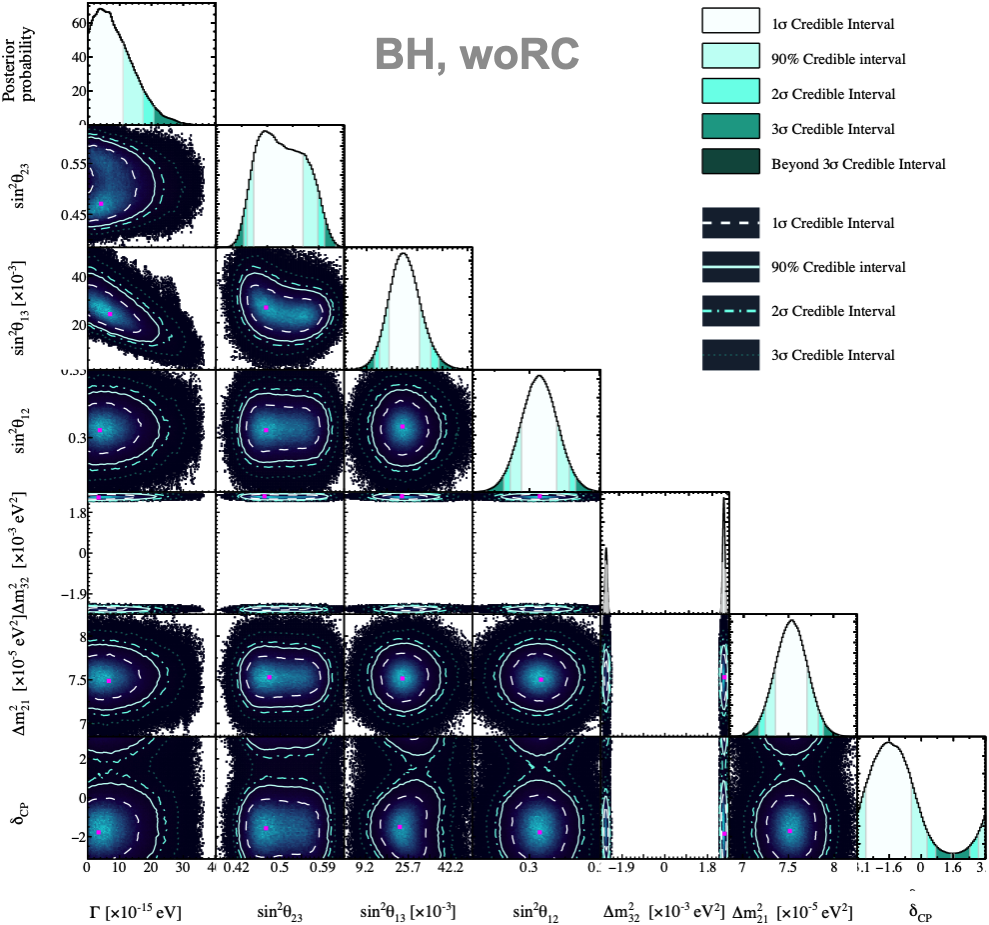
\includegraphics[width=1.\textwidth]{figures/TrianglePlots/T2K_A1/T2K_A1_QD_asimov_woRC_trianglePlot_bothMH.png}
    %{figures/TrianglePlots/T2K_A1/QD_asimov_woRC_trianglePlot_bothMH.pdf}
	\caption[Quantum Decoherence and Neutrino Oscillation Parameter Posterior Distributions of T2K A marginalised over \acrlong{bh} without Reactor Constraint with Non-Zero Decoherence Strength.]{The $1$- (upper plots) and $2$-dimensional posterior distributions of the oscillation parameters and decoherence strength from the T2K accelerator-neutrino fit marginalised over \acrfull{bh}. The $1\sigma$ (white, dashed), $90\%$ (light cyan, solid), $2\sigma$ (dark cyan, dotted-dashed), $3\sigma$ (green, dotted) and beyond $3\sigma$ (dark green) credible regions in the $1$-dimensional distributions are shown with the same colours in the $2$-dimensional contours. The Asimov point in this fit is $\left[ \sin^2(\theta_{12}), \sin^2(\theta_{23}), \sin^2(\theta_{13}), \Delta m^2_{12}, \Delta m^2_{23}, \delta_\text{CP}, \Gamma \right] =$ $\left[ 0.307, 0.561, 0.022, 7.53 \times 10{-3}, 2.494 \times 10^{-3}, -1.601, 5.0 \times 10 {-15} \right]$ (\textit{T2K Set A with non-zero decoherence strength}). The reactor constraint is not applied (woRC).}
	\label{fig:T2K_A1/QD_asimov_woRC_trianglePlot_bothMH}
    \end{figure}
%

%
    \begin{figure}[hbt]
	\centering
	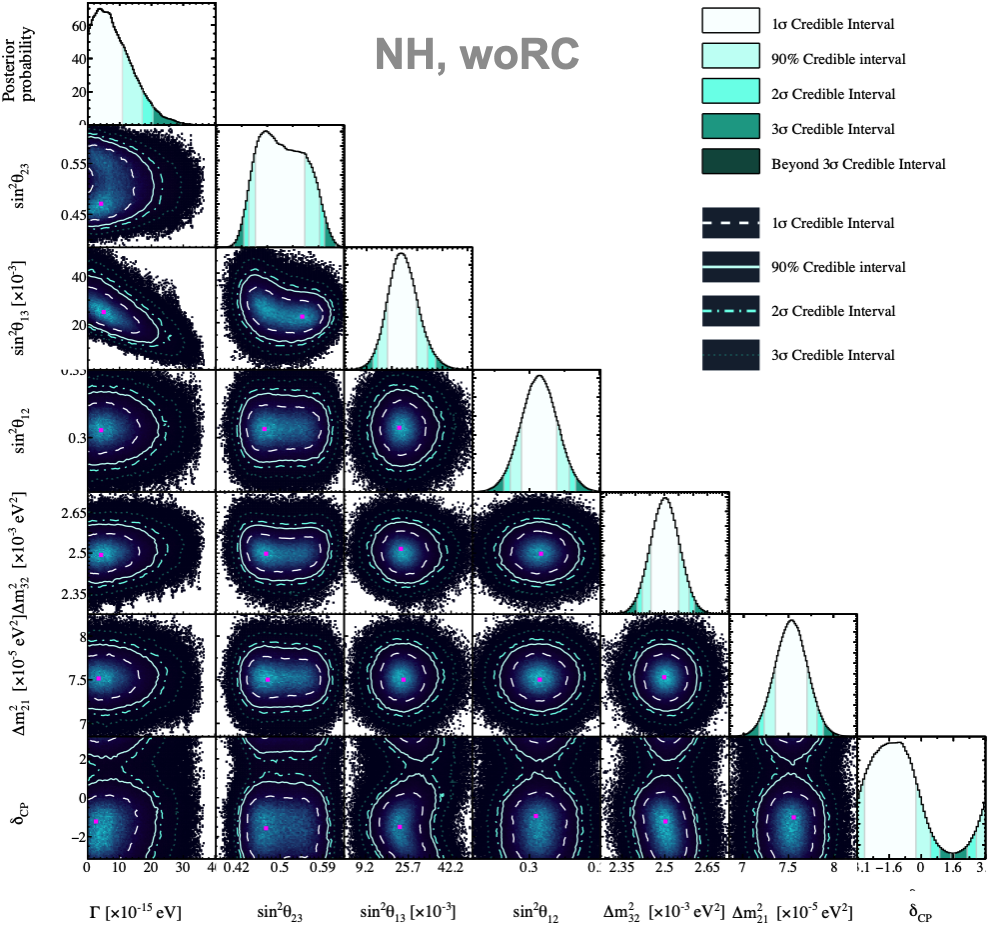
\includegraphics[width=1.\textwidth]{figures/TrianglePlots/T2K_A1/T2K_A1_QD_asimov_woRC_trianglePlot_nh.png}
    %{figures/TrianglePlots/T2K_A1/QD_asimov_woRC_trianglePlot_nh.pdf}
	\caption[Quantum Decoherence and Neutrino Oscillation Parameter Posterior Distributions of T2K A marginalised over the \acrlong{nh} without Reactor Constraint with Non-Zero Decoherence Strength.]{The $1$- (upper plots) and $2$-dimensional posterior distributions of the oscillation parameters and decoherence strength from the T2K accelerator-neutrino fit marginalised over the \acrfull{nh}. The $1\sigma$ (white, dashed), $90\%$ (light cyan, solid), $2\sigma$ (dark cyan, dotted-dashed), $3\sigma$ (green, dotted) and beyond $3\sigma$ (dark green) credible regions in the $1$-dimensional distributions are shown with the same colours in the $2$-dimensional contours. The Asimov point in this fit is $\left[ \sin^2(\theta_{12}), \sin^2(\theta_{23}), \sin^2(\theta_{13}), \Delta m^2_{12}, \Delta m^2_{23}, \delta_\text{CP}, \Gamma \right] =$ $\left[ 0.307, 0.561, 0.022, 7.53 \times 10{-3}, 2.494 \times 10^{-3}, -1.601, 5.0 \times 10 {-15} \right]$ (\textit{T2K Set A with non-zero decoherence strength}). The reactor constraint is not applied (woRC).}
	\label{fig:T2K_A1/QD_asimov_woRC_trianglePlot_nh}
    \end{figure}
%

%
    \begin{figure}[hbt]
	\centering
	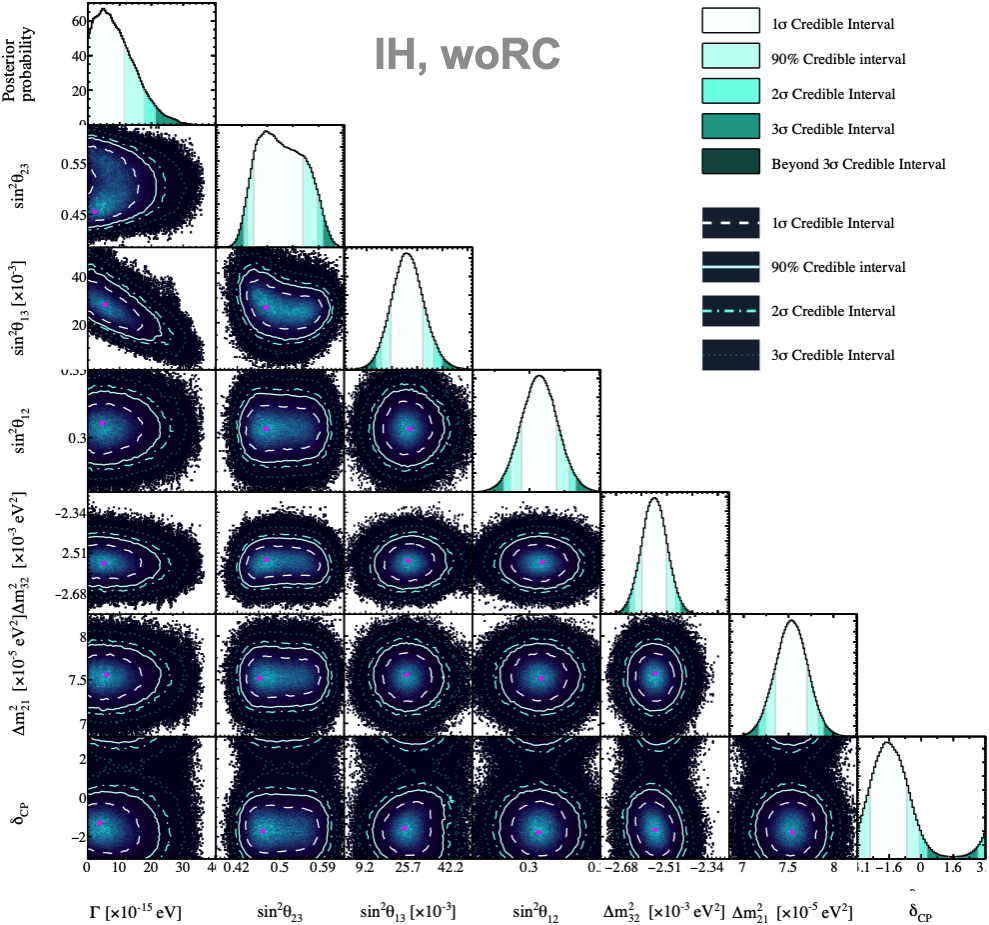
\includegraphics[width=1.\textwidth]{figures/TrianglePlots/T2K_A1/T2K_A1_QD_asimov_woRC_trianglePlot_ih.png}
    %{figures/TrianglePlots/T2K_A1/QD_asimov_woRC_trianglePlot_bothMH.pdf}
	\caption[Quantum Decoherence and Neutrino Oscillation Parameter Posterior Distributions of T2K A marginalised over the \acrlong{ih} without Reactor Constraint with Non-Zero Decoherence Strength.]{The $1$- (upper plots) and $2$-dimensional posterior distributions of the oscillation parameters and decoherence strength from the T2K accelerator-neutrino fit marginalised over the \acrfull{ih}. The $1\sigma$ (white, dashed), $90\%$ (light cyan, solid), $2\sigma$ (dark cyan, dotted-dashed), $3\sigma$ (green, dotted) and beyond $3\sigma$ (dark green) credible regions in the $1$-dimensional distributions are shown with the same colours in the $2$-dimensional contours. The Asimov point in this fit is $\left[ \sin^2(\theta_{12}), \sin^2(\theta_{23}), \sin^2(\theta_{13}), \Delta m^2_{12}, \Delta m^2_{23}, \delta_\text{CP}, \Gamma \right] =$ $\left[ 0.307, 0.561, 0.022, 7.53 \times 10{-3}, 2.494 \times 10^{-3}, -1.601, 5.0 \times 10 {-15} \right]$ (\textit{T2K Set A with non-zero decoherence strength}). The reactor constraint is not applied (woRC).}
	\label{fig:T2K_A1/QD_asimov_woRC_trianglePlot_ih}
    \end{figure}
%

%
    \begin{figure}[hbt]
	\centering
	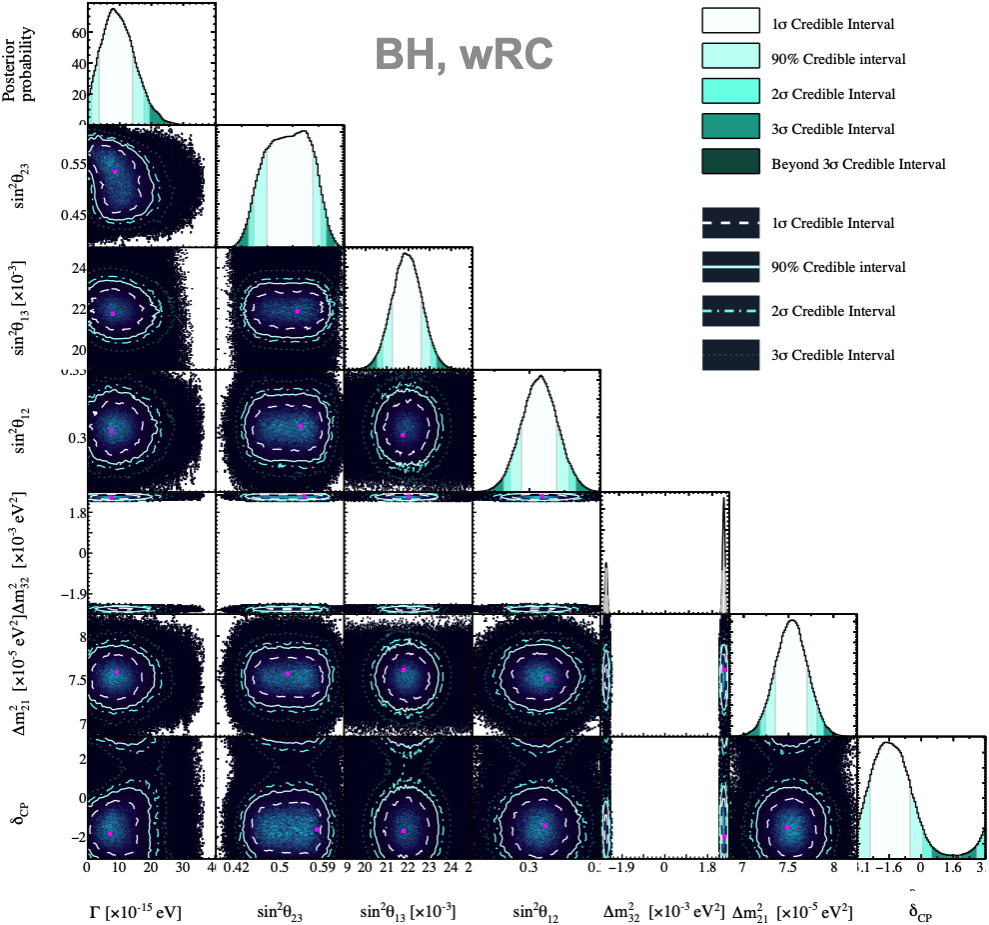
\includegraphics[width=1.\textwidth]{figures/TrianglePlots/T2K_A1/T2K_A1_QD_asimov_wRC_trianglePlot_bothMH.png}
    %{figures/TrianglePlots/T2K_A1/QD_asimov_woRC_trianglePlot_bothMH.pdf}
	\caption[Quantum Decoherence and Neutrino Oscillation Parameter Posterior Distributions of T2K A marginalised over \acrlong{bh} with Reactor Constraint with Non-Zero Decoherence Strength.]{The $1$- (upper plots) and $2$-dimensional posterior distributions of the oscillation parameters and decoherence strength from the T2K accelerator-neutrino fit marginalised over \acrfull{bh}. The $1\sigma$ (white, dashed), $90\%$ (light cyan, solid), $2\sigma$ (dark cyan, dotted-dashed), $3\sigma$ (green, dotted) and beyond $3\sigma$ (dark green) credible regions in the $1$-dimensional distributions are shown with the same colours in the $2$-dimensional contours. The Asimov point in this fit is $\left[ \sin^2(\theta_{12}), \sin^2(\theta_{23}), \sin^2(\theta_{13}), \Delta m^2_{12}, \Delta m^2_{23}, \delta_\text{CP}, \Gamma \right] =$ $\left[ 0.307, 0.561, 0.022, 7.53 \times 10{-3}, 2.494 \times 10^{-3}, -1.601, 5.0 \times 10 {-15} \right]$ (\textit{T2K Set A with non-zero decoherence strength}). The reactor constraint is applied (wRC).}
	\label{fig:T2K_A1/QD_asimov_wRC_trianglePlot_bothMH}
    \end{figure}
%

%
    \begin{figure}[hbt]
	\centering
	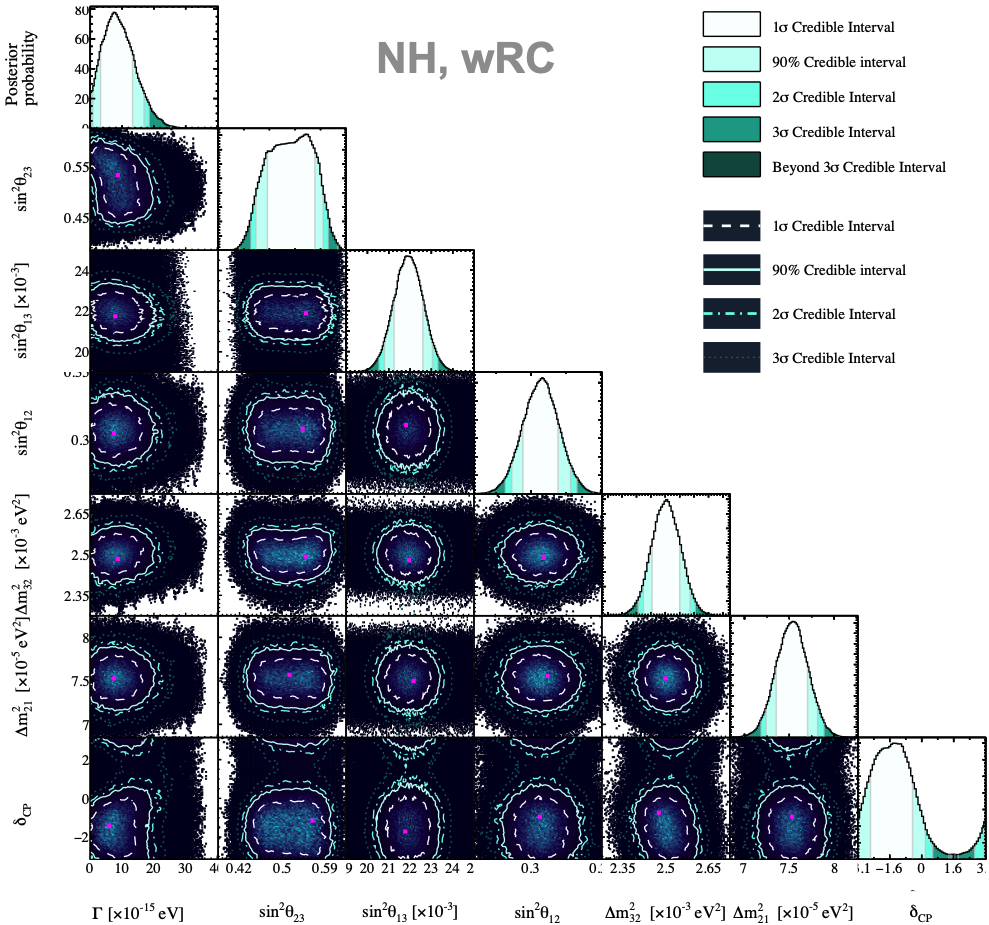
\includegraphics[width=1.\textwidth]{figures/TrianglePlots/T2K_A1/T2K_A1_QD_asimov_wRC_trianglePlot_nh.png}
    %{figures/TrianglePlots/T2K_A1/QD_asimov_woRC_trianglePlot_bothMH.pdf}
	\caption[Quantum Decoherence and Neutrino Oscillation Parameter Posterior Distributions of T2K A marginalised over the \acrlong{nh} with Reactor Constraint with Non-Zero Decoherence Strength.]{The $1$- (upper plots) and $2$-dimensional posterior distributions of the oscillation parameters and decoherence strength from the T2K accelerator-neutrino fit marginalised over the \acrfull{nh}. The $1\sigma$ (white, dashed), $90\%$ (light cyan, solid), $2\sigma$ (dark cyan, dotted-dashed), $3\sigma$ (green, dotted) and beyond $3\sigma$ (dark green) credible regions in the $1$-dimensional distributions are shown with the same colours in the $2$-dimensional contours. The Asimov point in this fit is $\left[ \sin^2(\theta_{12}), \sin^2(\theta_{23}), \sin^2(\theta_{13}), \Delta m^2_{12}, \Delta m^2_{23}, \delta_\text{CP}, \Gamma \right] =$ $\left[ 0.307, 0.561, 0.022, 7.53 \times 10{-3}, 2.494 \times 10^{-3}, -1.601, 5.0 \times 10 {-15} \right]$ (\textit{T2K Set A with non-zero decoherence strength}). The reactor constraint is applied (wRC).}
	\label{fig:T2K_A1/QD_asimov_wRC_trianglePlot_nh}
    \end{figure}
%

%
    \begin{figure}[hbt]
	\centering
	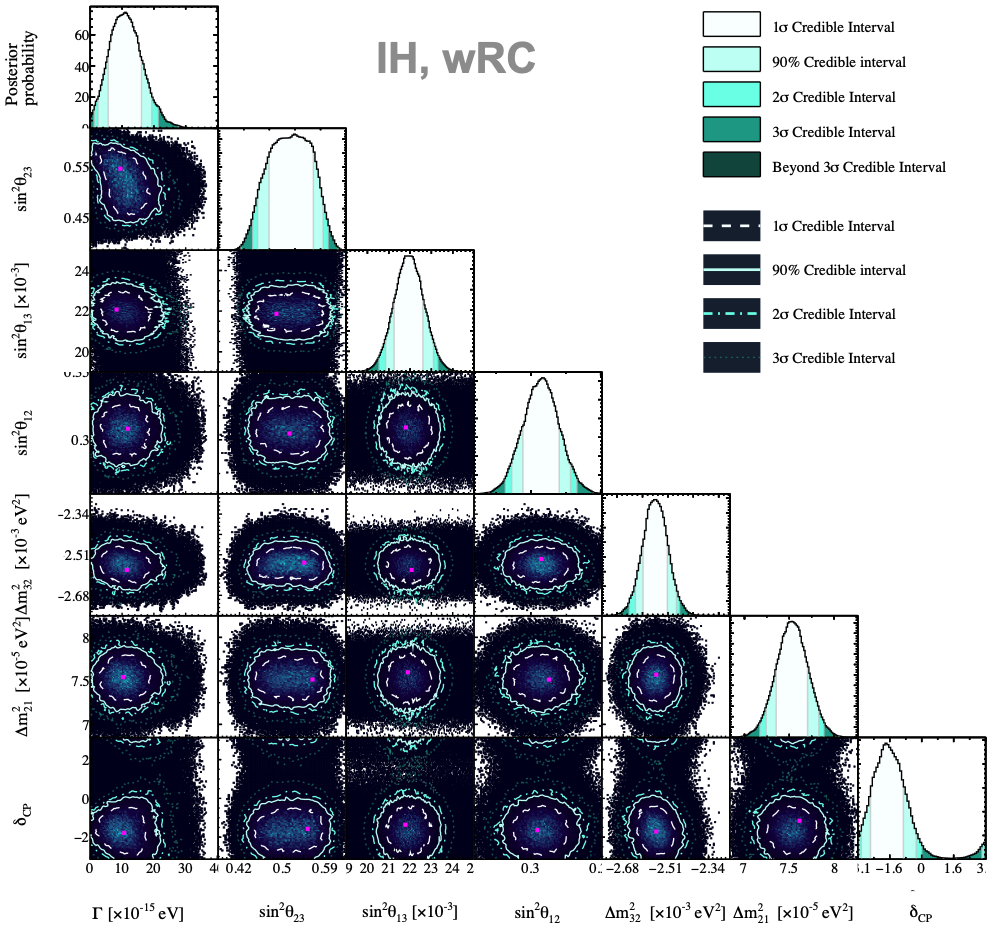
\includegraphics[width=1.\textwidth]{figures/TrianglePlots/T2K_A1/T2K_A1_QD_asimov_wRC_trianglePlot_ih.png}
    %{figures/TrianglePlots/T2K_A1/QD_asimov_woRC_trianglePlot_bothMH.pdf}
	\caption[Quantum Decoherence and Neutrino Oscillation Parameter Posterior Distributions of T2K A marginalised over the \acrlong{ih} with Reactor Constraint with Non-Zero Decoherence Strength.]{The $1$- (upper plots) and $2$-dimensional posterior distributions of the oscillation parameters and decoherence strength from the T2K accelerator-neutrino fit marginalised over the \acrfull{ih}. The $1\sigma$ (white, dashed), $90\%$ (light cyan, solid), $2\sigma$ (dark cyan, dotted-dashed), $3\sigma$ (green, dotted) and beyond $3\sigma$ (dark green) credible regions in the $1$-dimensional distributions are shown with the same colours in the $2$-dimensional contours. The Asimov point in this fit is $\left[ \sin^2(\theta_{12}), \sin^2(\theta_{23}), \sin^2(\theta_{13}), \Delta m^2_{12}, \Delta m^2_{23}, \delta_\text{CP}, \Gamma \right] =$ $\left[ 0.307, 0.561, 0.022, 7.53 \times 10{-3}, 2.494 \times 10^{-3}, -1.601, 5.0 \times 10 {-15} \right]$ (\textit{T2K Set A with non-zero decoherence strength}). The reactor constraint is applied (wRC).}
	\label{fig:T2K_A1/QD_asimov_wRC_trianglePlot_ih}
    \end{figure}
%
\newpage
%
    \begin{figure}[hbt]
	\centering
	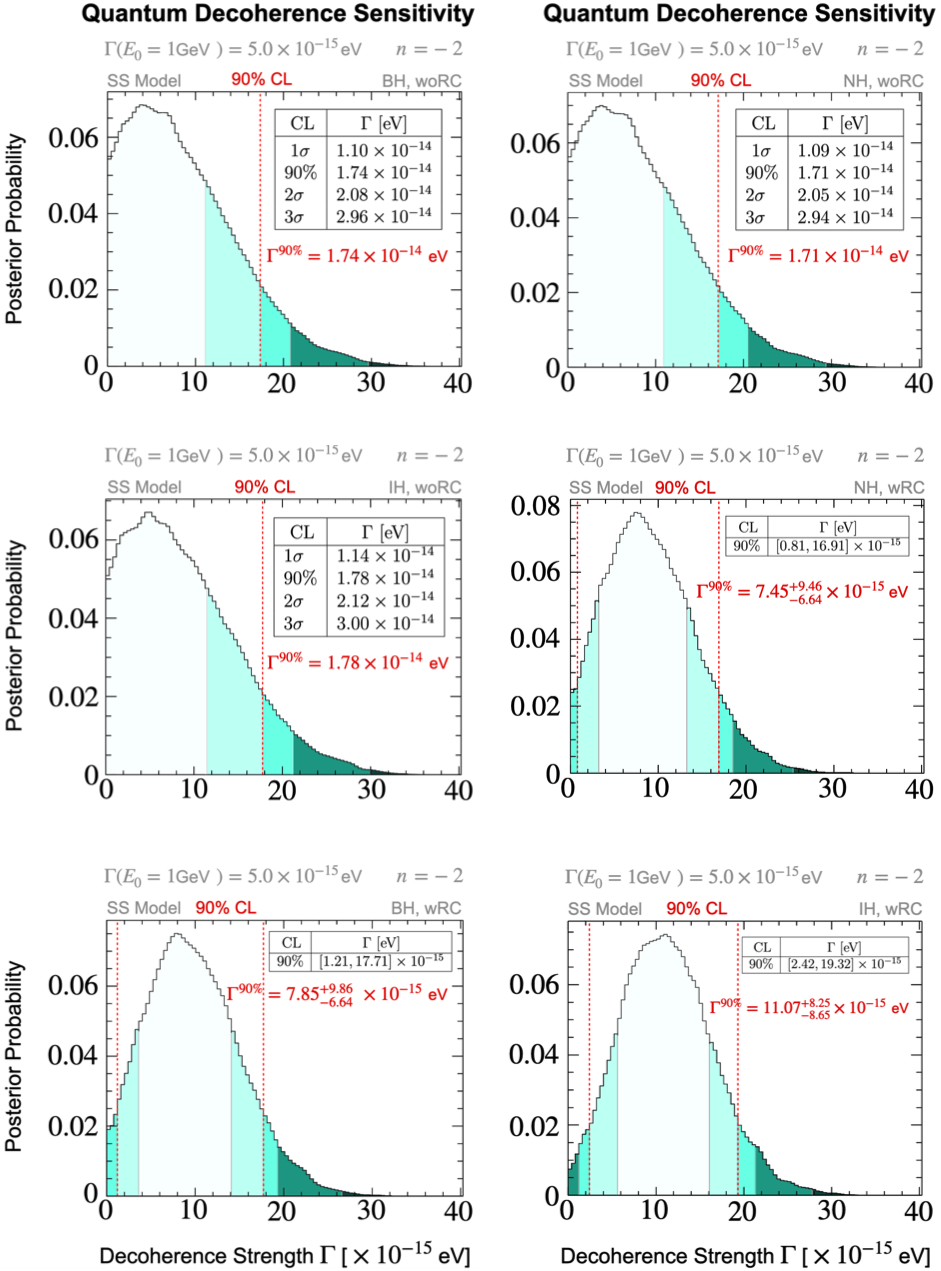
\includegraphics[width=1.\textwidth]{figures/TrianglePlots/T2K_A1/T2K_A1_QD_asimov_1d_decostrength_cis2.png}
    %{figures/TrianglePlots/T2K_A1/T2K_A1_QD_asimov_1d_decostrength_cis.png}
	\caption[Quantum Decoherence Posterior Distributions of T2K A with Non-Zero Decoherence Strength.]{Quantum decoherence posterior distributions of T2K A with non-zero decoherence strength as displayed in figs. \ref{fig:T2K_A1/QD_asimov_woRC_trianglePlot_bothMH}-\ref{fig:T2K_A1/QD_asimov_wRC_trianglePlot_ih}.}
    \label{fig:T2K_A1/T2K_A1_QD_asimov_1d_decostrength_cis}
    \end{figure}
%



%
\newpage
\subsection{T2K A with \texorpdfstring{$\mathbf{\Gamma = 0}$}{Gamma = 0}}
%% T2K Set A2
%
    \begin{figure}[hbt]
	\centering
	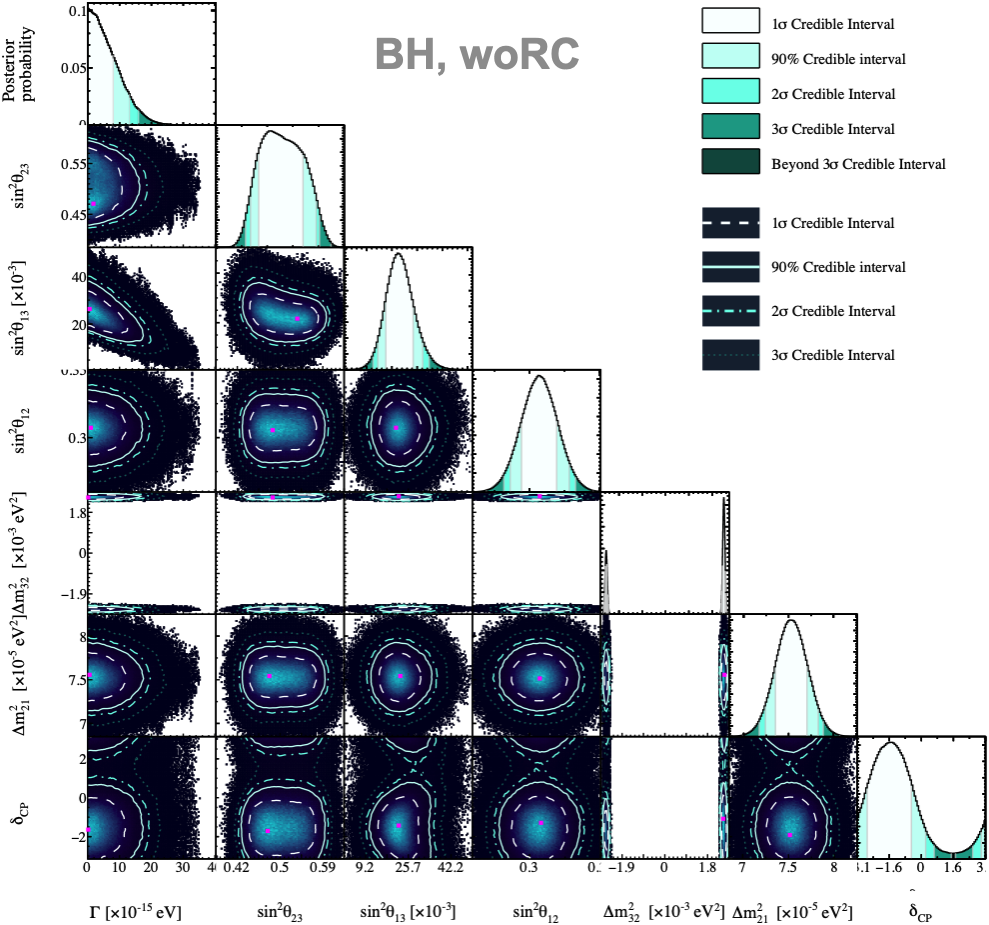
\includegraphics[width=1.\textwidth]{figures/TrianglePlots/T2K_A2/T2K_A2_QD_asimov_woRC_trianglePlot_bothMH.png}
    %{figures/TrianglePlots/T2K_A1/QD_asimov_woRC_trianglePlot_bothMH.pdf}
	\caption[Quantum Decoherence and Neutrino Oscillation Parameter Posterior Distributions of T2K A marginalised over \acrlong{bh} without Reactor Constraint with Zero Decoherence Strength.]{The $1$- (upper plots) and $2$-dimensional posterior distributions of the oscillation parameters and decoherence strength from the T2K accelerator-neutrino fit marginalised over \acrfull{bh}. The $1\sigma$ (white, dashed), $90\%$ (light cyan, solid), $2\sigma$ (dark cyan, dotted-dashed), $3\sigma$ (green, dotted) and beyond $3\sigma$ (dark green) credible regions in the $1$-dimensional distributions are shown with the same colours in the $2$-dimensional contours. The Asimov point in this fit is $\left[ \sin^2(\theta_{12}), \sin^2(\theta_{23}), \sin^2(\theta_{13}), \Delta m^2_{12}, \Delta m^2_{23}, \delta_\text{CP}, \Gamma \right] =$ $\left[ 0.307, 0.561, 0.022, 7.53 \times 10{-3}, 2.494 \times 10^{-3}, -1.601, 0.0 \right]$ (\textit{T2K Set A with zero decoherence strength}). The reactor constraint is not applied (woRC).}
	\label{fig:T2K_A2/QD_asimov_woRC_trianglePlot_bothMH}
    \end{figure}
%

%
    \begin{figure}[hbt]
	\centering
	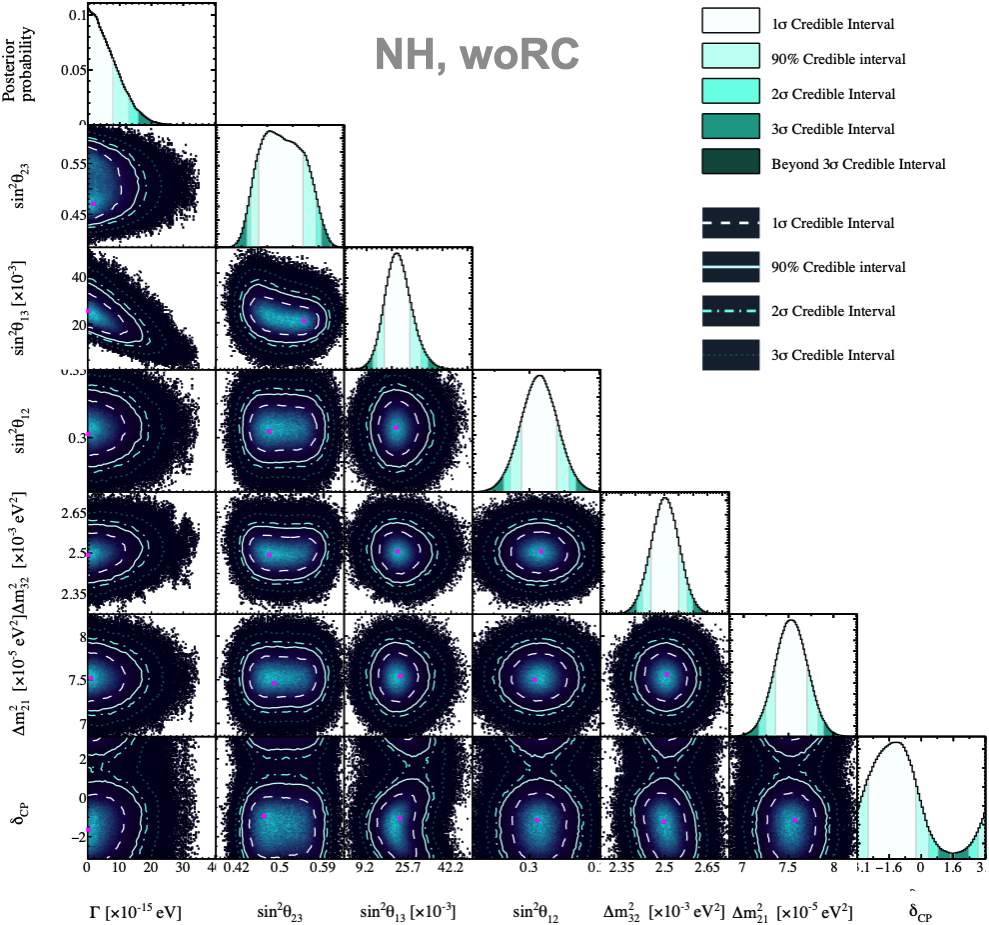
\includegraphics[width=1.\textwidth]{figures/TrianglePlots/T2K_A2/T2K_A2_QD_asimov_woRC_trianglePlot_nh.png}
    %{figures/TrianglePlots/T2K_A1/QD_asimov_woRC_trianglePlot_bothMH.pdf}
	\caption[Quantum Decoherence and Neutrino Oscillation Parameter Posterior Distributions of T2K A marginalised over the \acrlong{nh} without Reactor Constraint with Zero Decoherence Strength.]{The $1$- (upper plots) and $2$-dimensional posterior distributions of the oscillation parameters and decoherence strength from the T2K accelerator-neutrino fit marginalised over the \acrfull{nh}. The $1\sigma$ (white, dashed), $90\%$ (light cyan, solid), $2\sigma$ (dark cyan, dotted-dashed), $3\sigma$ (green, dotted) and beyond $3\sigma$ (dark green) credible regions in the $1$-dimensional distributions are shown with the same colours in the $2$-dimensional contours. The Asimov point in this fit is $\left[ \sin^2(\theta_{12}), \sin^2(\theta_{23}), \sin^2(\theta_{13}), \Delta m^2_{12}, \Delta m^2_{23}, \delta_\text{CP}, \Gamma \right] =$ $\left[ 0.307, 0.561, 0.022, 7.53 \times 10{-3}, 2.494 \times 10^{-3}, -1.601, 0.0 \right]$ (\textit{T2K Set A with zero decoherence strength}). The reactor constraint is not applied (woRC).}
	\label{fig:T2K_A2/QD_asimov_woRC_trianglePlot_nh}
    \end{figure}
%

%
    \begin{figure}[hbt]
	\centering
	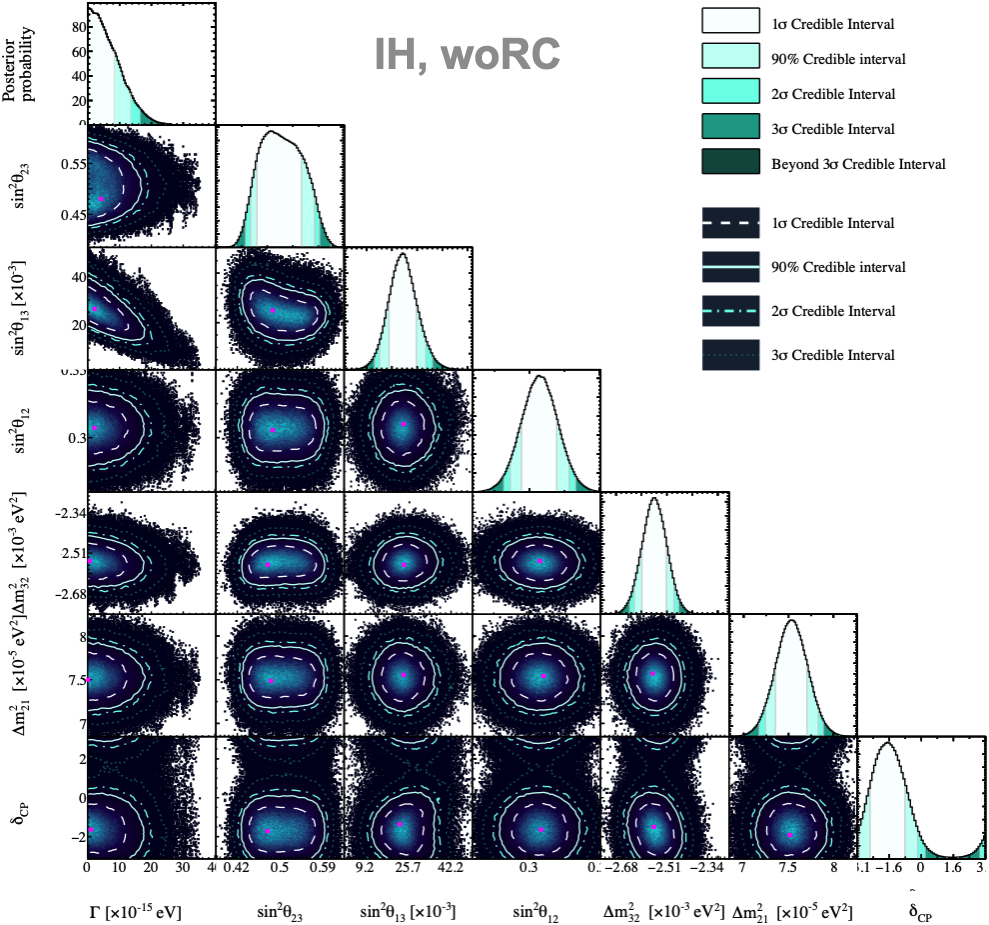
\includegraphics[width=1.\textwidth]{figures/TrianglePlots/T2K_A2/T2K_A2_QD_asimov_woRC_trianglePlot_ih.png}
    %{figures/TrianglePlots/T2K_A1/QD_asimov_woRC_trianglePlot_bothMH.pdf}
	\caption[Quantum Decoherence and Neutrino Oscillation Parameter Posterior Distributions of T2K A marginalised over the \acrlong{ih} without Reactor Constraint with Zero Decoherence Strength.]{The $1$- (upper plots) and $2$-dimensional posterior distributions of the oscillation parameters and decoherence strength from the T2K accelerator-neutrino fit marginalised over the \acrfull{ih}. The $1\sigma$ (white, dashed), $90\%$ (light cyan, solid), $2\sigma$ (dark cyan, dotted-dashed), $3\sigma$ (green, dotted) and beyond $3\sigma$ (dark green) credible regions in the $1$-dimensional distributions are shown with the same colours in the $2$-dimensional contours. The Asimov point in this fit is $\left[ \sin^2(\theta_{12}), \sin^2(\theta_{23}), \sin^2(\theta_{13}), \Delta m^2_{12}, \Delta m^2_{23}, \delta_\text{CP}, \Gamma \right] =$ $\left[ 0.307, 0.561, 0.022, 7.53 \times 10{-3}, 2.494 \times 10^{-3}, -1.601, 0.0 \right]$ (\textit{T2K Set A with zero decoherence strength}). The reactor constraint is not applied (woRC).}
	\label{fig:T2K_A2/QD_asimov_woRC_trianglePlot_ih}
    \end{figure}
%

%
    \begin{figure}[hbt]
	\centering
	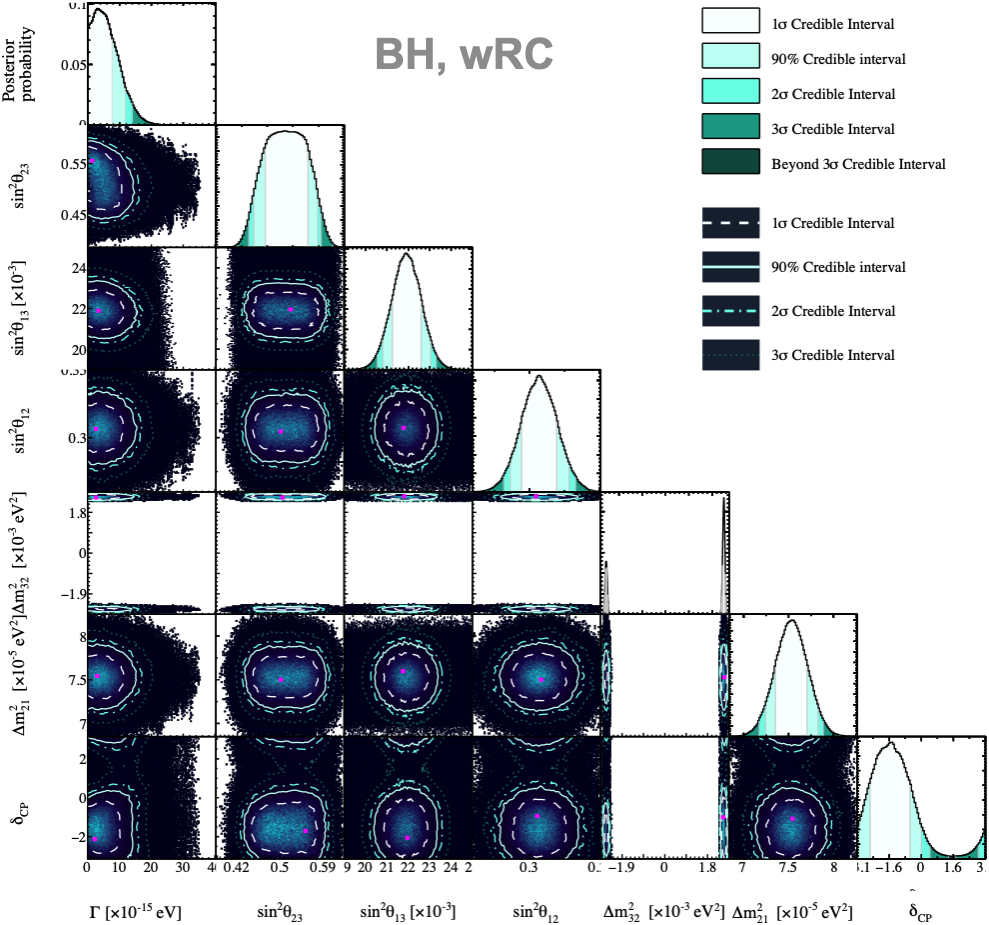
\includegraphics[width=1.\textwidth]{figures/TrianglePlots/T2K_A2/T2K_A2_QD_asimov_wRC_trianglePlot_bothMH.png}
    %{figures/TrianglePlots/T2K_A1/QD_asimov_woRC_trianglePlot_bothMH.pdf}
	\caption[Quantum Decoherence and Neutrino Oscillation Parameter Posterior Distributions of T2K A marginalised over \acrlong{bh} with Reactor Constraint with Zero Decoherence Strength.]{The $1$- (upper plots) and $2$-dimensional posterior distributions of the oscillation parameters and decoherence strength from the T2K accelerator-neutrino fit marginalised over \acrfull{bh}. The $1\sigma$ (white, dashed), $90\%$ (light cyan, solid), $2\sigma$ (dark cyan, dotted-dashed), $3\sigma$ (green, dotted) and beyond $3\sigma$ (dark green) credible regions in the $1$-dimensional distributions are shown with the same colours in the $2$-dimensional contours. The Asimov point in this fit is $\left[ \sin^2(\theta_{12}), \sin^2(\theta_{23}), \sin^2(\theta_{13}), \Delta m^2_{12}, \Delta m^2_{23}, \delta_\text{CP}, \Gamma \right] =$ $\left[ 0.307, 0.561, 0.022, 7.53 \times 10{-3}, 2.494 \times 10^{-3}, -1.601, 0.0 \right]$ (\textit{T2K Set A with zero decoherence strength}). The reactor constraint is applied (wRC).}
	\label{fig:T2K_A2/QD_asimov_wRC_trianglePlot_bothMH}
    \end{figure}
%

%
    \begin{figure}[hbt]
	\centering
	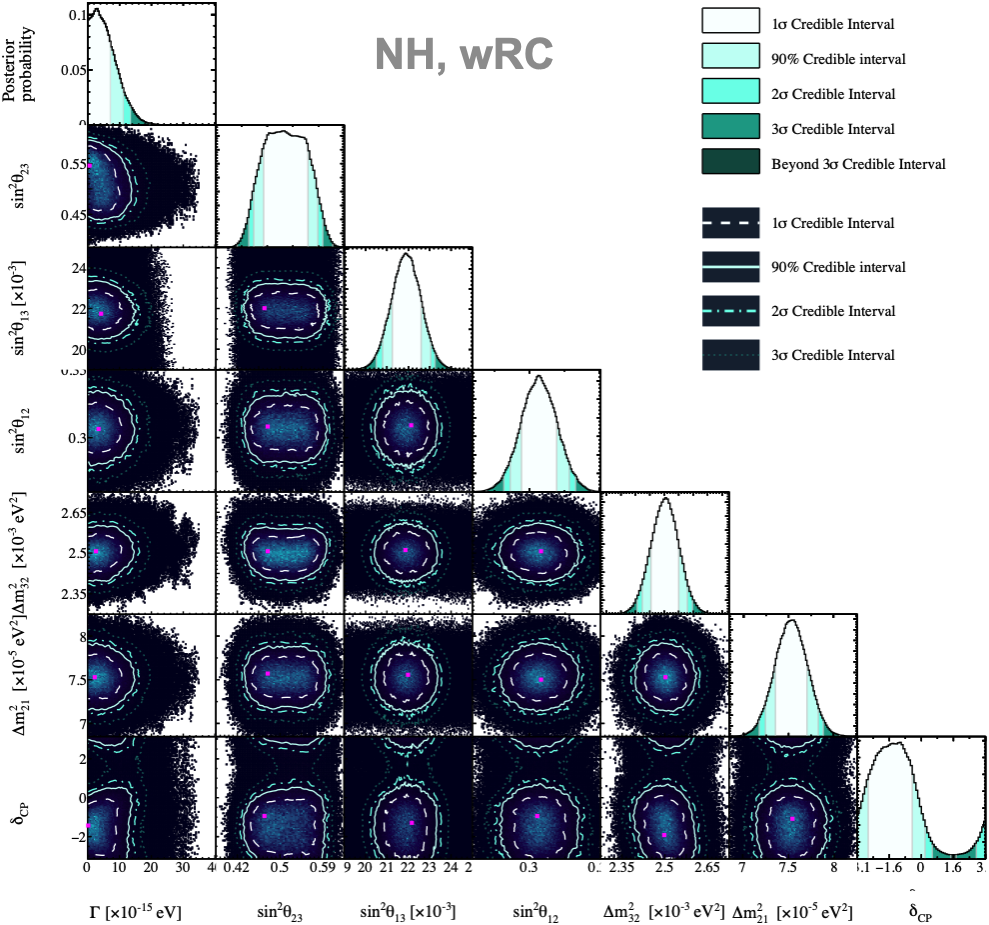
\includegraphics[width=1.\textwidth]{figures/TrianglePlots/T2K_A2/T2K_A2_QD_asimov_wRC_trianglePlot_nh.png}
    %{figures/TrianglePlots/T2K_A1/QD_asimov_woRC_trianglePlot_bothMH.pdf}
	\caption[Quantum Decoherence and Neutrino Oscillation Parameter Posterior Distributions of T2K A marginalised over the \acrlong{nh} with Reactor Constraint with Zero Decoherence Strength.]{The $1$- (upper plots) and $2$-dimensional posterior distributions of the oscillation parameters and decoherence strength from the T2K accelerator-neutrino fit marginalised over the \acrfull{nh}. The $1\sigma$ (white, dashed), $90\%$ (light cyan, solid), $2\sigma$ (dark cyan, dotted-dashed), $3\sigma$ (green, dotted) and beyond $3\sigma$ (dark green) credible regions in the $1$-dimensional distributions are shown with the same colours in the $2$-dimensional contours. The Asimov point in this fit is $\left[ \sin^2(\theta_{12}), \sin^2(\theta_{23}), \sin^2(\theta_{13}), \Delta m^2_{12}, \Delta m^2_{23}, \delta_\text{CP}, \Gamma \right] =$ $\left[ 0.307, 0.561, 0.022, 7.53 \times 10{-3}, 2.494 \times 10^{-3}, -1.601, 0.0 \right]$ (\textit{T2K Set A with zero decoherence strength}). The reactor constraint is applied (wRC).}
	\label{fig:T2K_A2/QD_asimov_wRC_trianglePlot_nh}
    \end{figure}
%

%
    \begin{figure}[hbt]
	\centering
	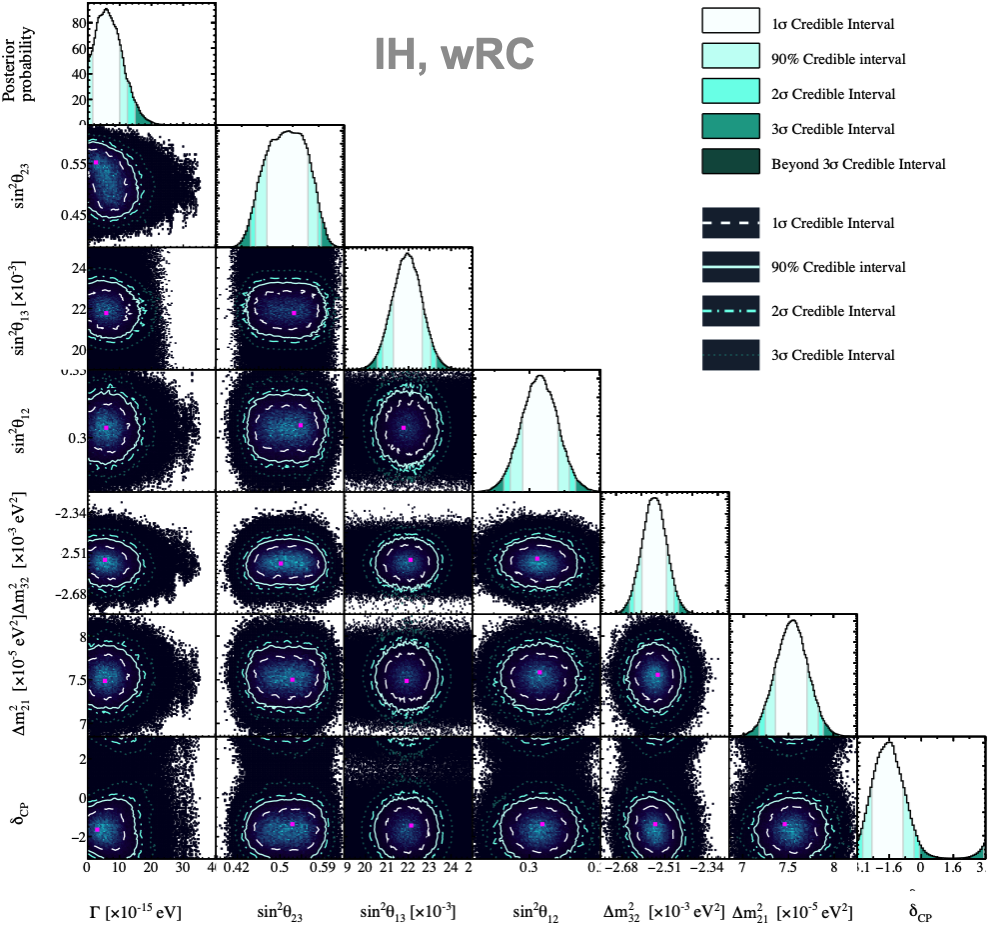
\includegraphics[width=1.\textwidth]{figures/TrianglePlots/T2K_A2/T2K_A2_QD_asimov_wRC_trianglePlot_ih.png}
    %{figures/TrianglePlots/T2K_A1/QD_asimov_woRC_trianglePlot_bothMH.pdf}
	\caption[Quantum Decoherence and Neutrino Oscillation Parameter Posterior Distributions of T2K A marginalised over the \acrlong{ih} with Reactor Constraint with Zero Decoherence Strength.]{The $1$- (upper plots) and $2$-dimensional posterior distributions of the oscillation parameters and decoherence strength from the T2K accelerator-neutrino fit marginalised over the \acrfull{ih}. The $1\sigma$ (white, dashed), $90\%$ (light cyan, solid), $2\sigma$ (dark cyan, dotted-dashed), $3\sigma$ (green, dotted) and beyond $3\sigma$ (dark green) credible regions in the $1$-dimensional distributions are shown with the same colours in the $2$-dimensional contours. The Asimov point in this fit is $\left[ \sin^2(\theta_{12}), \sin^2(\theta_{23}), \sin^2(\theta_{13}), \Delta m^2_{12}, \Delta m^2_{23}, \delta_\text{CP}, \Gamma \right] =$ $\left[ 0.307, 0.561, 0.022, 7.53 \times 10{-3}, 2.494 \times 10^{-3}, -1.601, 0.0 \right]$ (\textit{T2K Set A with zero decoherence strength}). The reactor constraint is applied (wRC).}
	\label{fig:T2K_A2/QD_asimov_wRC_trianglePlot_ih}
    \end{figure}
%
%
    \begin{figure}[hbt]
	\centering
	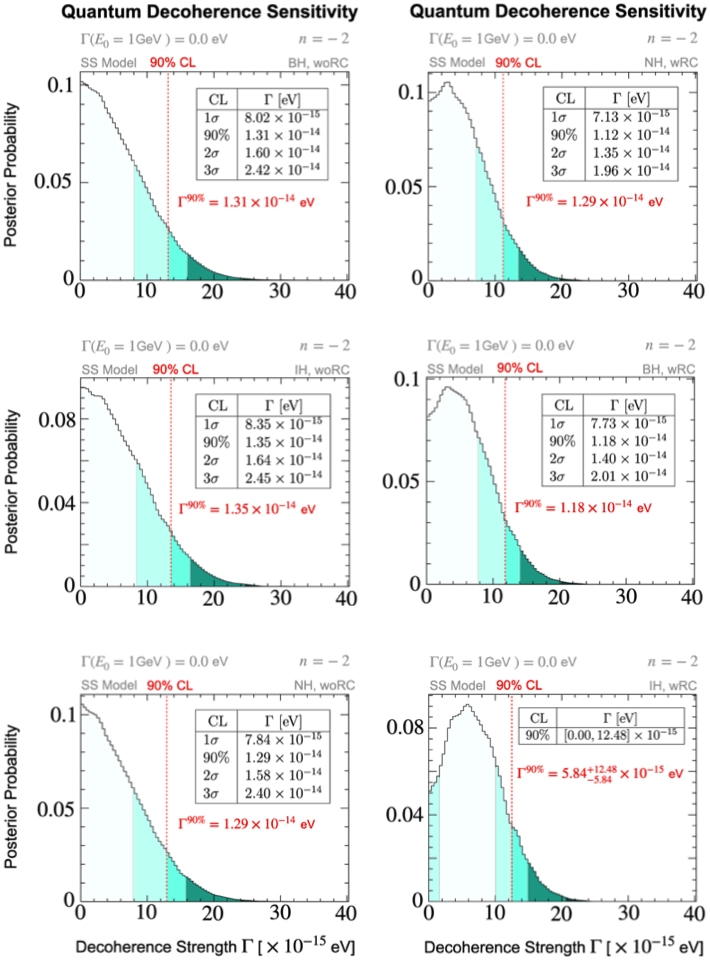
\includegraphics[width=1.\textwidth]{figures/TrianglePlots/T2K_A2/T2K_A2_QD_asimov_1d_decostrength_cis2.png}
    %{figures/TrianglePlots/T2K_A2/T2K_A2_QD_asimov_1d_decostrength_cis.png}
	\caption[Quantum Decoherence Posterior Distributions of T2K A with Zero Decoherence Strength.]{Quantum decoherence posterior distributions of T2K A with zero decoherence strength as displayed in figs. \ref{fig:T2K_A2/QD_asimov_woRC_trianglePlot_bothMH}-\ref{fig:T2K_A2/QD_asimov_wRC_trianglePlot_ih}.}
    \label{fig:T2K_A2/T2K_A2_QD_asimov_1d_decostrength_cis}
    \end{figure}
%


%
\newpage
\subsection{T2K B with \texorpdfstring{$\mathbf{\Gamma \neq 0}$}{Gamma = 0}}
%% T2K Set B3
%
    \begin{figure}[hbt]
	\centering
	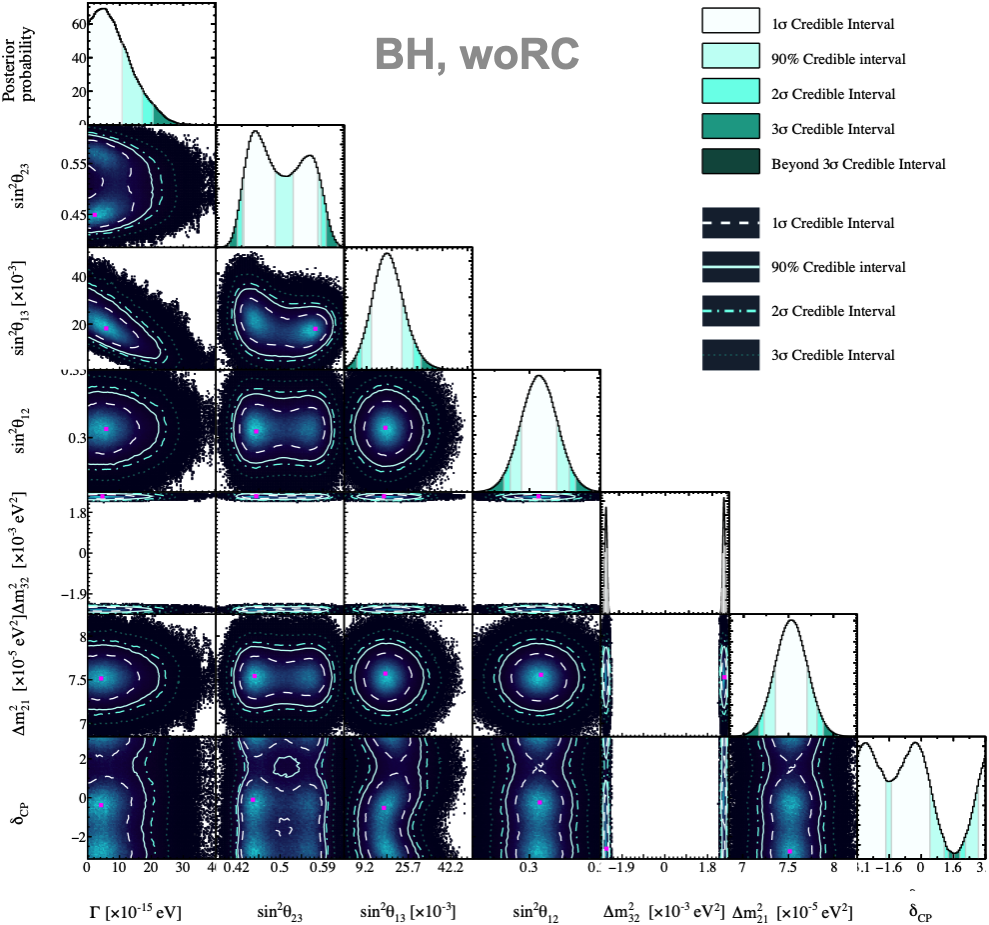
\includegraphics[width=1.\textwidth]{figures/TrianglePlots/T2K_B3/T2K_B3_QD_asimov_woRC_trianglePlot_bothMH.png}
    %{figures/TrianglePlots/T2K_B3/QD_asimov_woRC_trianglePlot_bothMH.pdf}
	\caption[Quantum Decoherence and Neutrino Oscillation Parameter Posterior Distributions of T2K B marginalised over \acrlong{bh} without Reactor Constraint with Non-Zero Decoherence Strength.]{The $1$- (upper plots) and $2$-dimensional posterior distributions of the oscillation parameters and decoherence strength from the T2K accelerator-neutrino fit marginalised over \acrfull{bh}. The $1\sigma$ (white, dashed), $90\%$ (light cyan, solid), $2\sigma$ (dark cyan, dotted-dashed), $3\sigma$ (green, dotted) and beyond $3\sigma$ (dark green) credible regions in the $1$-dimensional distributions are shown with the same colours in the $2$-dimensional contours. The Asimov point in this fit is $\left[ \sin^2(\theta_{12}), \sin^2(\theta_{23}), \sin^2(\theta_{13}), \Delta m^2_{12}, \Delta m^2_{23}, \delta_\text{CP}, \Gamma \right] =$ $\left[ 0.307, 0.450, 0.022, 7.53 \times 10{-3}, 2.494 \times 10^{-3}, 0.0, 5.0 \times 10 {-15} \right]$ (\textit{T2K Set B with non-zero decoherence strength}). The reactor constraint is not applied (woRC).}
	\label{fig:T2K_B3/QD_asimov_woRC_trianglePlot_bothMH}
    \end{figure}
%

%
    \begin{figure}[hbt]
	\centering
	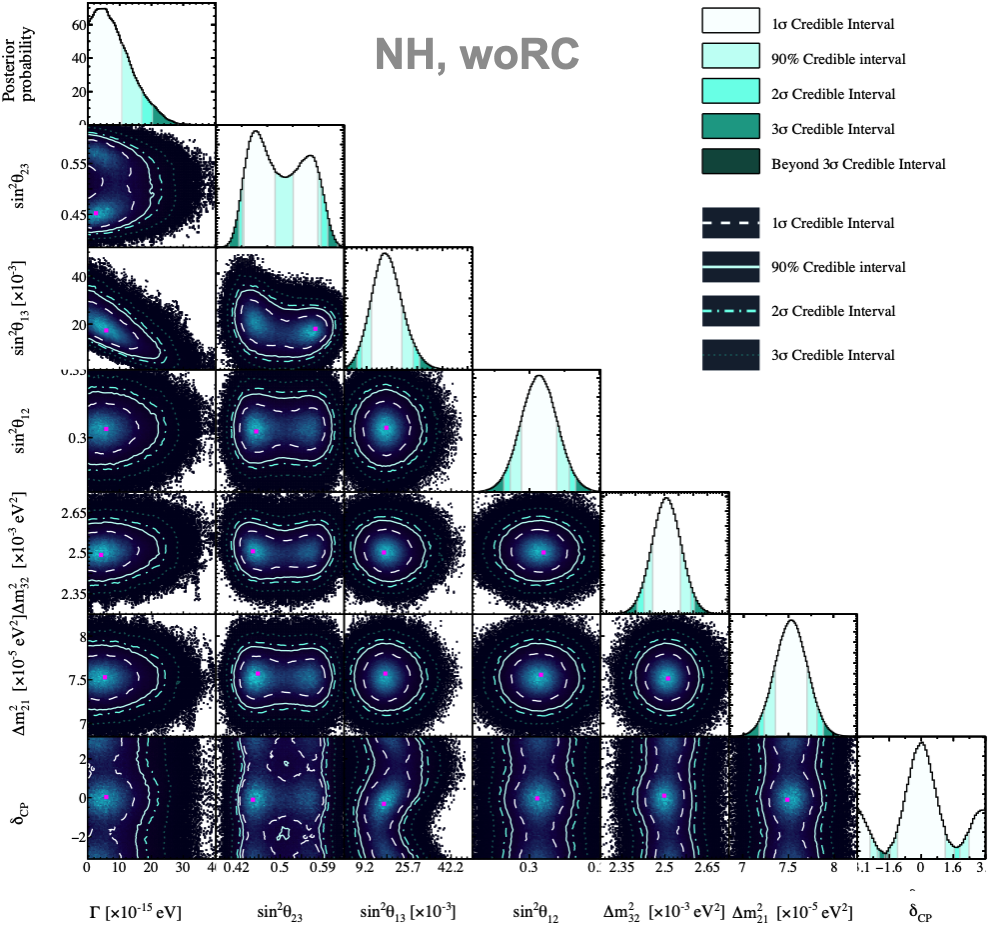
\includegraphics[width=1.\textwidth]{figures/TrianglePlots/T2K_B3/T2K_B3_QD_asimov_woRC_trianglePlot_nh.png}
    %{figures/TrianglePlots/T2K_B3/QD_asimov_woRC_trianglePlot_bothMH.pdf}
	\caption[Quantum Decoherence and Neutrino Oscillation Parameter Posterior Distributions of T2K B marginalised over the \acrlong{nh} without Reactor Constraint with Non-Zero Decoherence Strength.]{The $1$- (upper plots) and $2$-dimensional posterior distributions of the oscillation parameters and decoherence strength from the T2K accelerator-neutrino fit marginalised over the \acrfull{nh}. The $1\sigma$ (white, dashed), $90\%$ (light cyan, solid), $2\sigma$ (dark cyan, dotted-dashed), $3\sigma$ (green, dotted) and beyond $3\sigma$ (dark green) credible regions in the $1$-dimensional distributions are shown with the same colours in the $2$-dimensional contours. The Asimov point in this fit is $\left[ \sin^2(\theta_{12}), \sin^2(\theta_{23}), \sin^2(\theta_{13}), \Delta m^2_{12}, \Delta m^2_{23}, \delta_\text{CP}, \Gamma \right] =$ $\left[ 0.307, 0.450, 0.022, 7.53 \times 10{-3}, 2.494 \times 10^{-3}, 0.0, 5.0 \times 10 {-15} \right]$ (\textit{T2K Set B with non-zero decoherence strength}). The reactor constraint is not applied (woRC).}
	\label{fig:T2K_B3/QD_asimov_woRC_trianglePlot_nh}
    \end{figure}
%

%
    \begin{figure}[hbt]
	\centering
	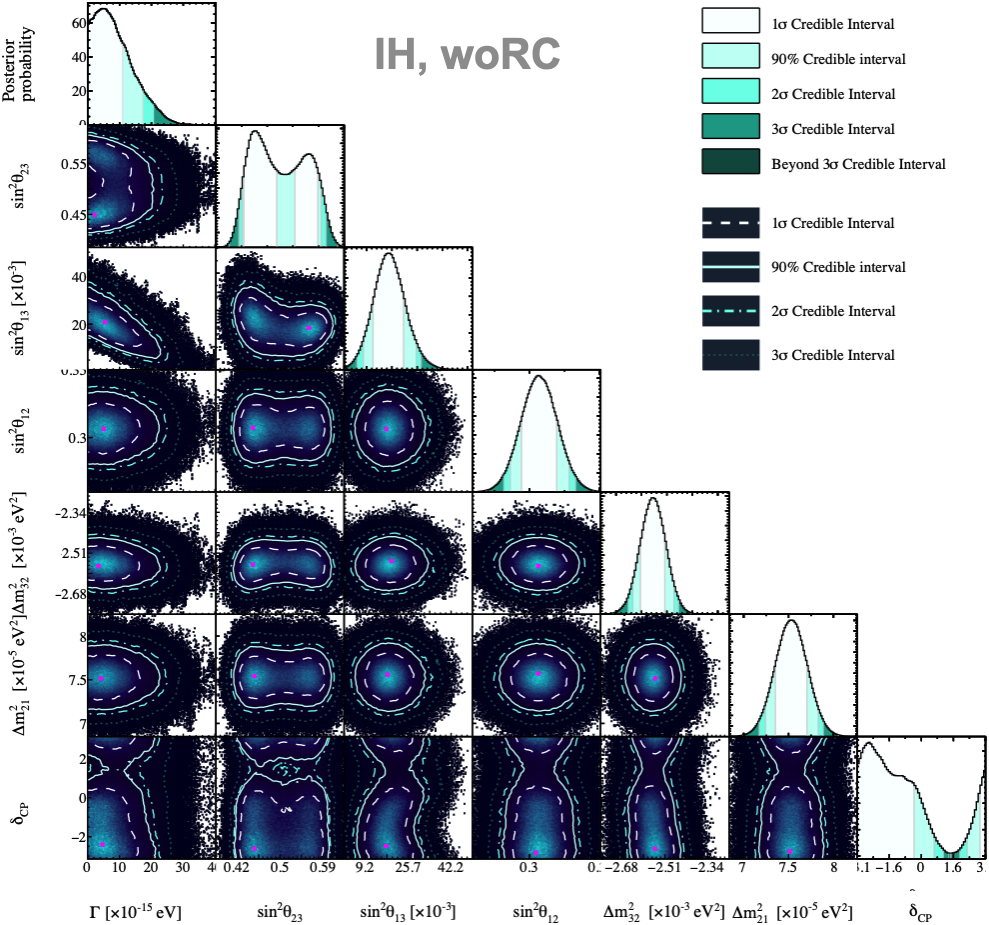
\includegraphics[width=1.\textwidth]{figures/TrianglePlots/T2K_B3/T2K_B3_QD_asimov_woRC_trianglePlot_ih.png}
    %{figures/TrianglePlots/T2K_A1/QD_asimov_woRC_trianglePlot_bothMH.pdf}
	\caption[Quantum Decoherence and Neutrino Oscillation Parameter Posterior Distributions of T2K B marginalised over the \acrlong{ih} without Reactor Constraint with Non-Zero Decoherence Strength.]{The $1$- (upper plots) and $2$-dimensional posterior distributions of the oscillation parameters and decoherence strength from the T2K accelerator-neutrino fit marginalised over the \acrfull{ih}. The $1\sigma$ (white, dashed), $90\%$ (light cyan, solid), $2\sigma$ (dark cyan, dotted-dashed), $3\sigma$ (green, dotted) and beyond $3\sigma$ (dark green) credible regions in the $1$-dimensional distributions are shown with the same colours in the $2$-dimensional contours. The Asimov point in this fit is $\left[ \sin^2(\theta_{12}), \sin^2(\theta_{23}), \sin^2(\theta_{13}), \Delta m^2_{12}, \Delta m^2_{23}, \delta_\text{CP}, \Gamma \right] =$ $\left[ 0.307, 0.450, 0.022, 7.53 \times 10{-3}, 2.494 \times 10^{-3}, 0.0, 5.0 \times 10 {-15} \right]$ (\textit{T2K Set B with non-zero decoherence strength}). The reactor constraint is not applied (woRC).}
	\label{fig:T2K_B3/QD_asimov_woRC_trianglePlot_ih}
    \end{figure}
%

%
    \begin{figure}[hbt]
	\centering
	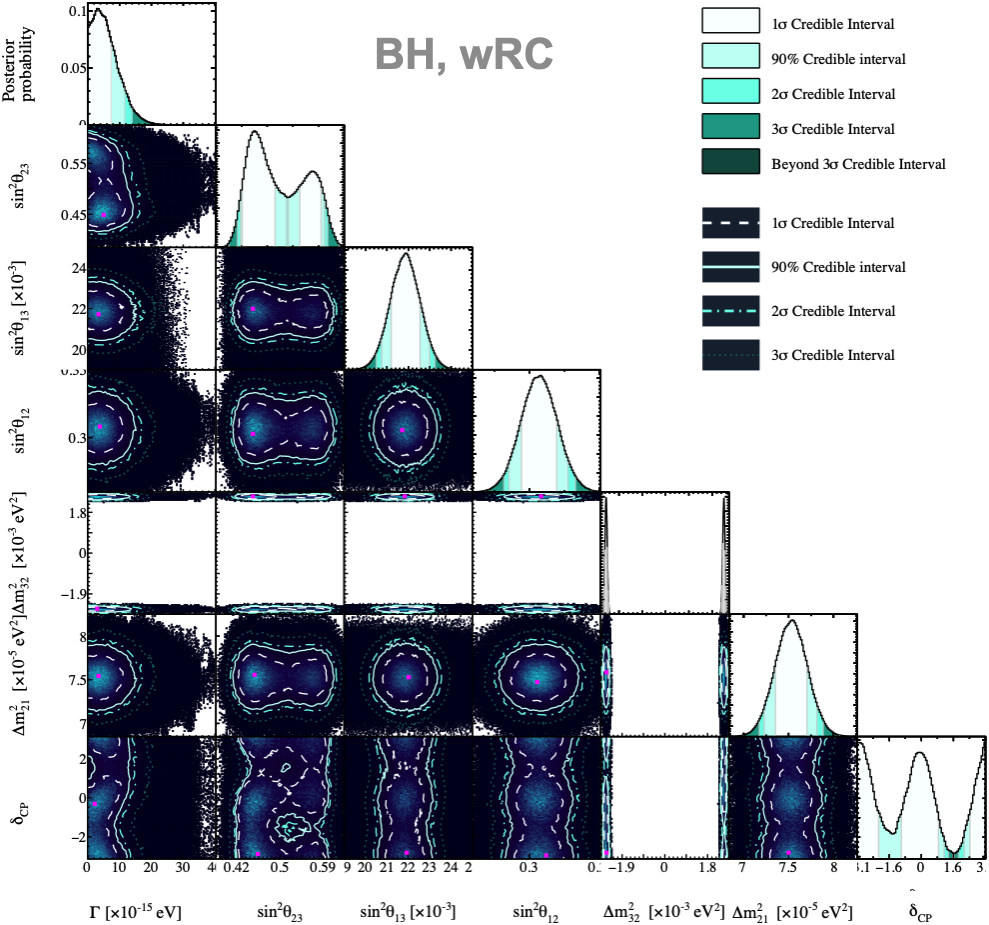
\includegraphics[width=1.\textwidth]{figures/TrianglePlots/T2K_B3/T2K_B3_QD_asimov_wRC_trianglePlot_bothMH.png}
    %{figures/TrianglePlots/T2K_B3/QD_asimov_woRC_trianglePlot_bothMH.pdf}
	\caption[Quantum Decoherence and Neutrino Oscillation Parameter Posterior Distributions of T2K B marginalised over \acrlong{bh} with Reactor Constraint with Non-Zero Decoherence Strength.]{The $1$- (upper plots) and $2$-dimensional posterior distributions of the oscillation parameters and decoherence strength from the T2K accelerator-neutrino fit marginalised over \acrfull{bh}. The $1\sigma$ (white, dashed), $90\%$ (light cyan, solid), $2\sigma$ (dark cyan, dotted-dashed), $3\sigma$ (green, dotted) and beyond $3\sigma$ (dark green) credible regions in the $1$-dimensional distributions are shown with the same colours in the $2$-dimensional contours. The Asimov point in this fit is $\left[ \sin^2(\theta_{12}), \sin^2(\theta_{23}), \sin^2(\theta_{13}), \Delta m^2_{12}, \Delta m^2_{23}, \delta_\text{CP}, \Gamma \right] =$ $\left[ 0.307, 0.450, 0.022, 7.53 \times 10{-3}, 2.494 \times 10^{-3}, 0.0, 5.0 \times 10 {-15} \right]$ (\textit{T2K Set B with non-zero decoherence strength}). The reactor constraint is applied (wRC).}
	\label{fig:T2K_B3/QD_asimov_wRC_trianglePlot_bothMH}
    \end{figure}
%

%
    \begin{figure}[hbt]
	\centering
	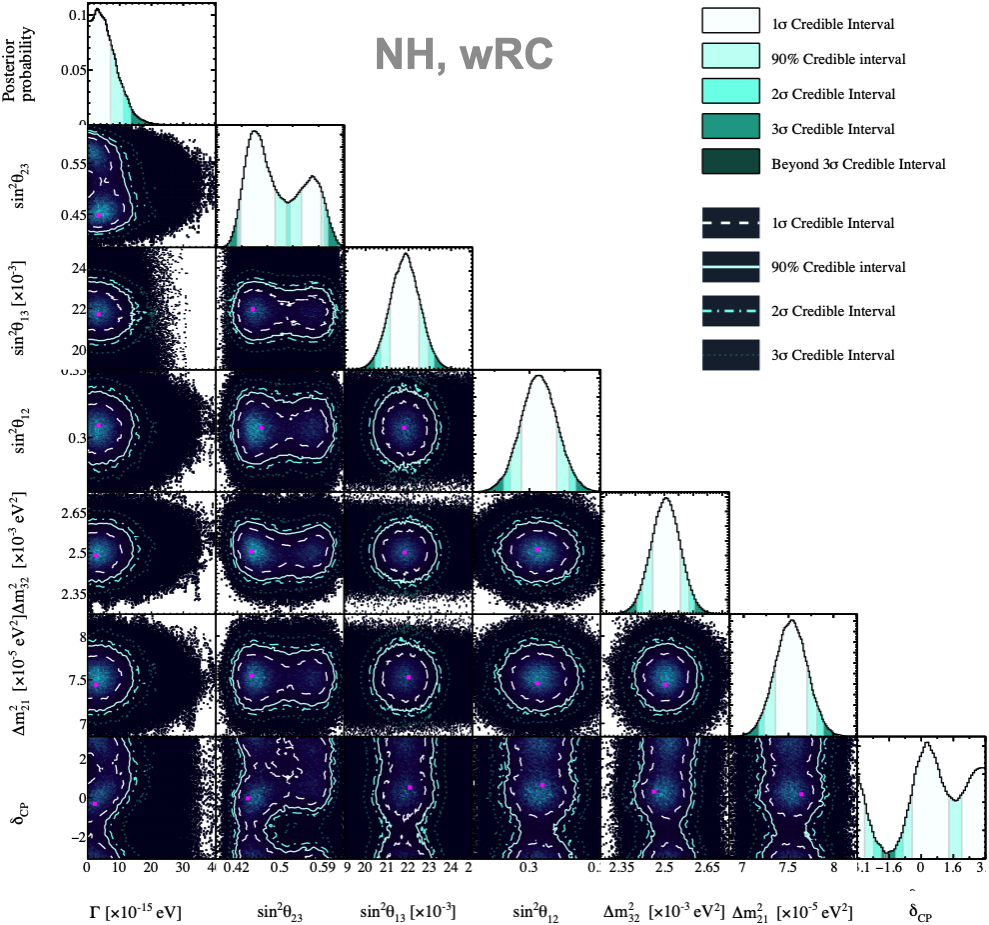
\includegraphics[width=1.\textwidth]{figures/TrianglePlots/T2K_B3/T2K_B3_QD_asimov_wRC_trianglePlot_nh.png}
    %{figures/TrianglePlots/T2K_B3/QD_asimov_woRC_trianglePlot_bothMH.pdf}
	\caption[Quantum Decoherence and Neutrino Oscillation Parameter Posterior Distributions of T2K B marginalised over the \acrlong{nh} with Reactor Constraint with Non-Zero Decoherence Strength.]{The $1$- (upper plots) and $2$-dimensional posterior distributions of the oscillation parameters and decoherence strength from the T2K accelerator-neutrino fit marginalised over the \acrfull{nh}. The $1\sigma$ (white, dashed), $90\%$ (light cyan, solid), $2\sigma$ (dark cyan, dotted-dashed), $3\sigma$ (green, dotted) and beyond $3\sigma$ (dark green) credible regions in the $1$-dimensional distributions are shown with the same colours in the $2$-dimensional contours. The Asimov point in this fit is $\left[ \sin^2(\theta_{12}), \sin^2(\theta_{23}), \sin^2(\theta_{13}), \Delta m^2_{12}, \Delta m^2_{23}, \delta_\text{CP}, \Gamma \right] =$ $\left[ 0.307, 0.450, 0.022, 7.53 \times 10{-3}, 2.494 \times 10^{-3}, 0.0, 5.0 \times 10 {-15} \right]$ (\textit{T2K Set B with non-zero decoherence strength}). The reactor constraint is applied (wRC).}
	\label{fig:T2K_B3/QD_asimov_wRC_trianglePlot_nh}
    \end{figure}
%

%
    \begin{figure}[hbt]
	\centering
	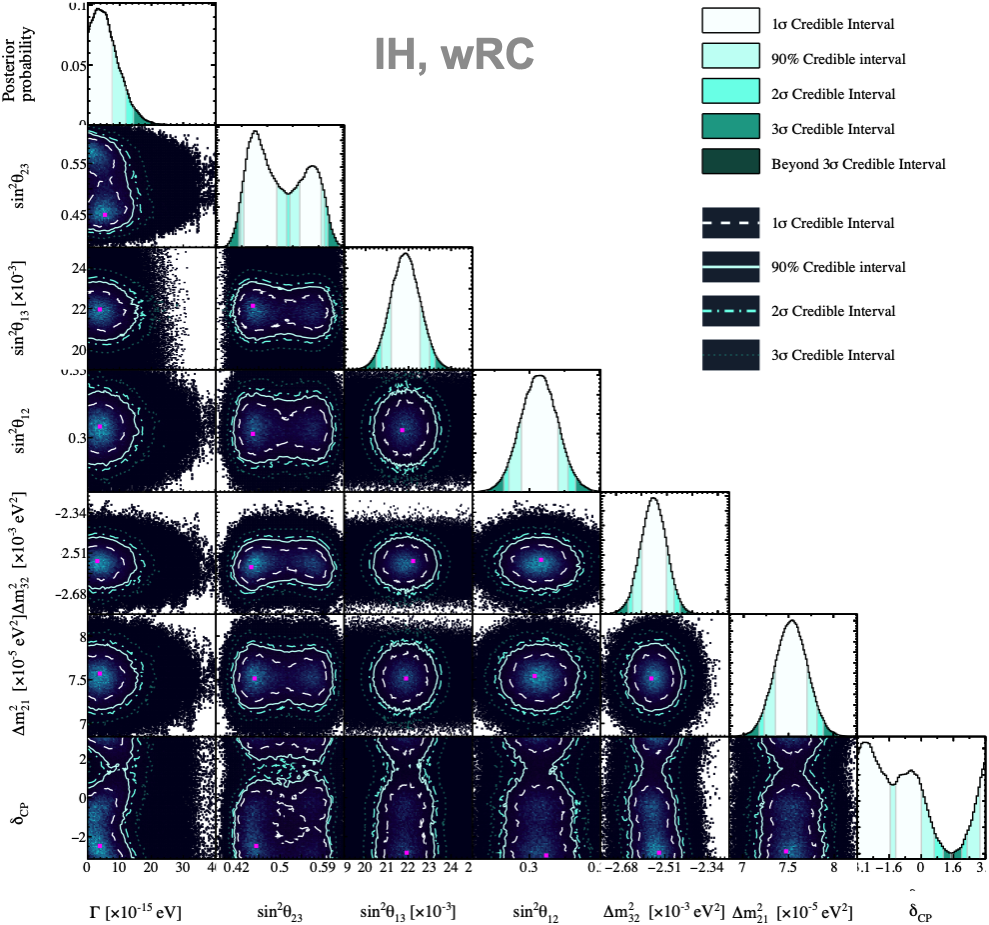
\includegraphics[width=1.\textwidth]{figures/TrianglePlots/T2K_B3/T2K_B3_QD_asimov_wRC_trianglePlot_ih.png}
    %{figures/TrianglePlots/T2K_B3/QD_asimov_woRC_trianglePlot_bothMH.pdf}
	\caption[Quantum Decoherence and Neutrino Oscillation Parameter Posterior Distributions of T2K B marginalised over the \acrlong{ih} with Reactor Constraint with Non-Zero Decoherence Strength.]{The $1$- (upper plots) and $2$-dimensional posterior distributions of the oscillation parameters and decoherence strength from the T2K accelerator-neutrino fit marginalised over the \acrfull{ih}. The $1\sigma$ (white, dashed), $90\%$ (light cyan, solid), $2\sigma$ (dark cyan, dotted-dashed), $3\sigma$ (green, dotted) and beyond $3\sigma$ (dark green) credible regions in the $1$-dimensional distributions are shown with the same colours in the $2$-dimensional contours. The Asimov point in this fit is $\left[ \sin^2(\theta_{12}), \sin^2(\theta_{23}), \sin^2(\theta_{13}), \Delta m^2_{12}, \Delta m^2_{23}, \delta_\text{CP}, \Gamma \right] =$ $\left[ 0.307, 0.450, 0.022, 7.53 \times 10{-3}, 2.494 \times 10^{-3}, 0.0, 5.0 \times 10 {-15} \right]$ (\textit{T2K Set B with non-zero decoherence strength}). The reactor constraint is applied (wRC).}
	\label{fig:T2K_B3/QD_asimov_wRC_trianglePlot_ih}
    \end{figure}
%

%
    \begin{figure}[hbt]
	\centering
	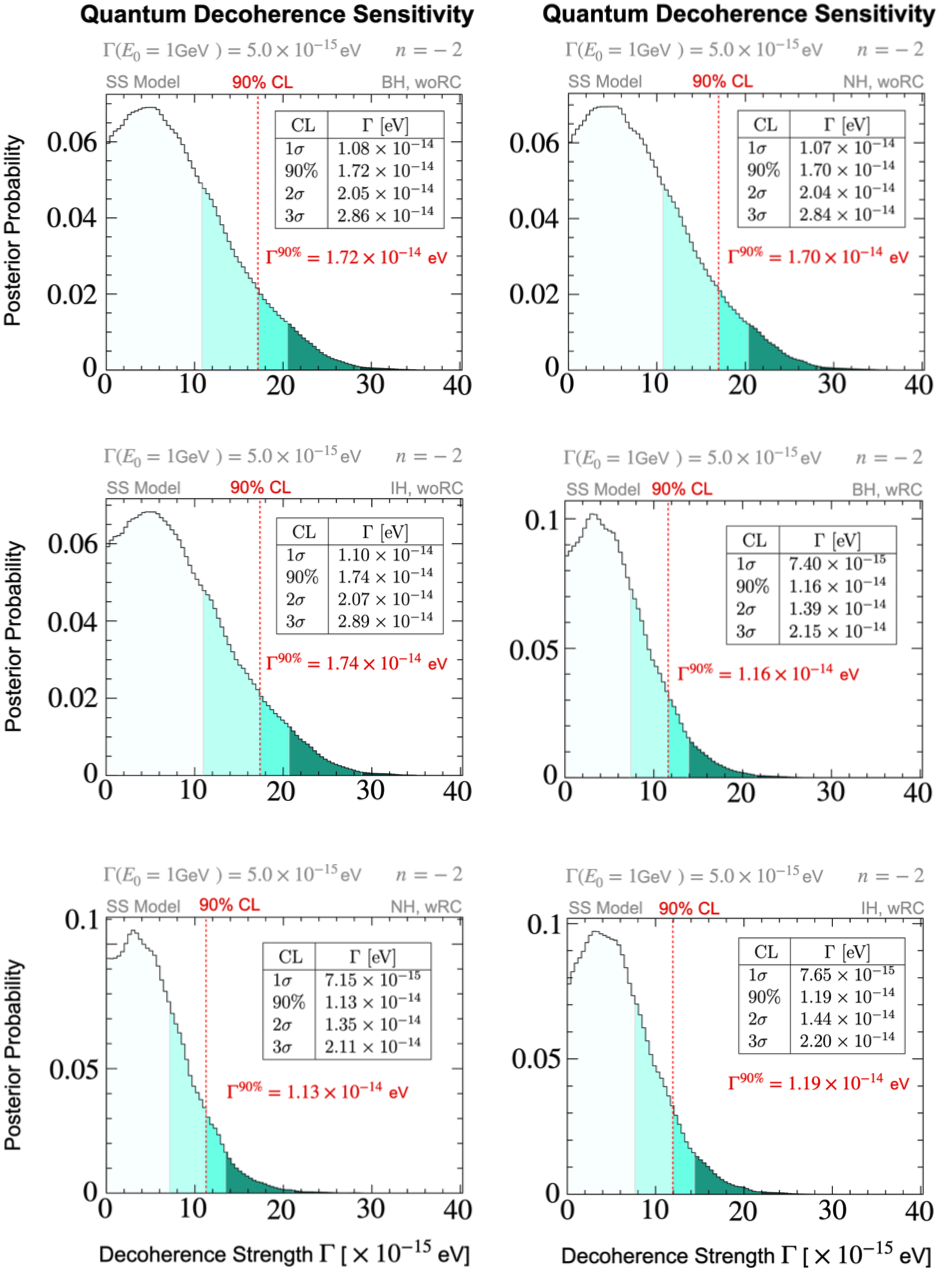
\includegraphics[width=1.\textwidth]{figures/TrianglePlots/T2K_B3/T2K_B3_QD_asimov_1d_decostrength_cis2.png}
    %{figures/TrianglePlots/T2K_B3/T2K_B3_QD_asimov_1d_decostrength_cis.png}
	\caption[Quantum Decoherence Posterior Distributions of T2K B with Non-Zero Decoherence Strength.]{Quantum decoherence posterior distributions of T2K B with non-zero decoherence strength as displayed in figs. \ref{fig:T2K_B3/QD_asimov_woRC_trianglePlot_bothMH}-\ref{fig:T2K_B3/QD_asimov_wRC_trianglePlot_ih}.}
    \label{fig:T2K_A2/T2K_A2_QD_asimov_1d_decostrength_cis}
    \end{figure}
%

\newpage
%
\subsection{T2K B with \texorpdfstring{$\mathbf{\Gamma = 0}$}{Gamma = 0}}
%% T2K Set B4
%
    \begin{figure}[hbt]
	\centering
	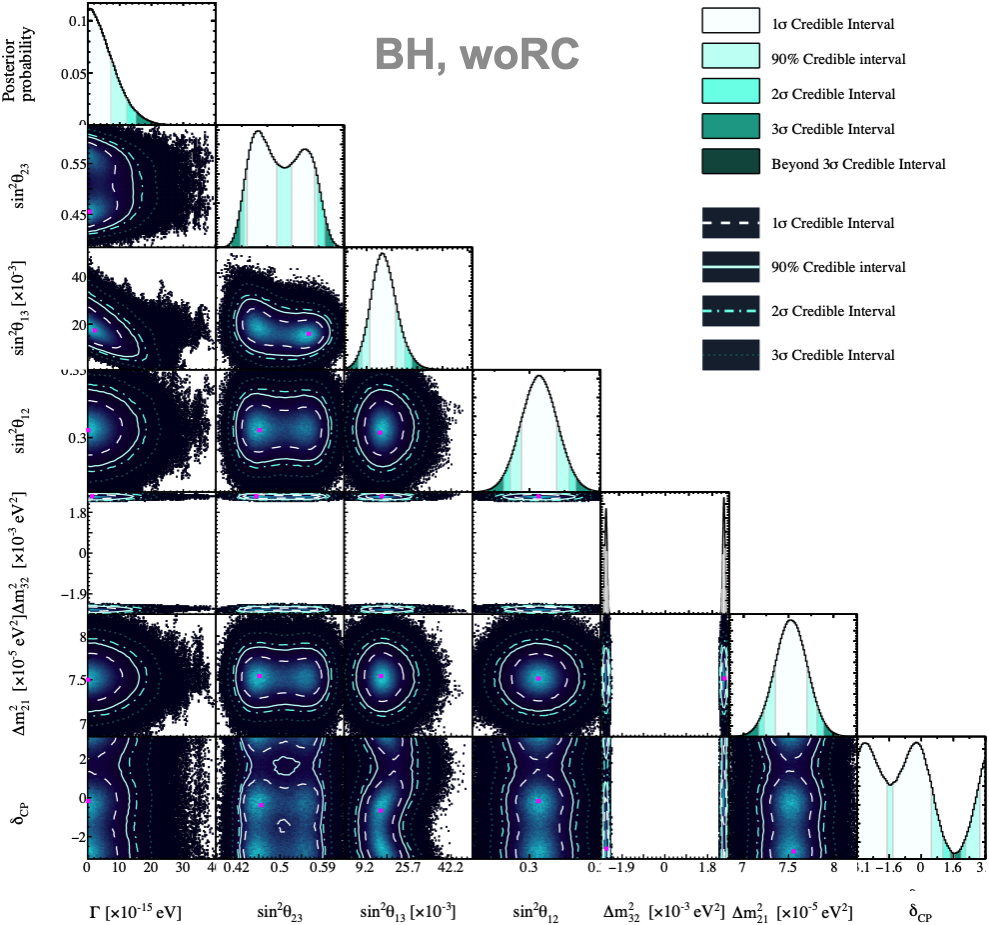
\includegraphics[width=1.\textwidth]{figures/TrianglePlots/T2K_B4/T2K_B4_QD_asimov_woRC_trianglePlot_bothMH.png}
    %{figures/TrianglePlots/T2K_B4/QD_asimov_woRC_trianglePlot_bothMH.pdf}
	\caption[Quantum Decoherence and Neutrino Oscillation Parameter Posterior Distributions of T2K B marginalised over \acrlong{bh} without Reactor Constraint with Zero Decoherence Strength.]{The $1$- (upper plots) and $2$-dimensional posterior distributions of the oscillation parameters and decoherence strength from the T2K accelerator-neutrino fit marginalised over \acrfull{bh}. The $1\sigma$ (white, dashed), $90\%$ (light cyan, solid), $2\sigma$ (dark cyan, dotted-dashed), $3\sigma$ (green, dotted) and beyond $3\sigma$ (dark green) credible regions in the $1$-dimensional distributions are shown with the same colours in the $2$-dimensional contours. The Asimov point in this fit is $\left[ \sin^2(\theta_{12}), \sin^2(\theta_{23}), \sin^2(\theta_{13}), \Delta m^2_{12}, \Delta m^2_{23}, \delta_\text{CP}, \Gamma \right] =$ $\left[ 0.307, 0.450, 0.022, 7.53 \times 10{-3}, 2.494 \times 10^{-3}, 0.0, 0.0 \right]$ (\textit{T2K Set B with zero decoherence strength}). The reactor constraint is not applied (woRC).}
	\label{fig:T2K_B4/QD_asimov_woRC_trianglePlot_bothMH}
    \end{figure}
%

%
    \begin{figure}[hbt]
	\centering
	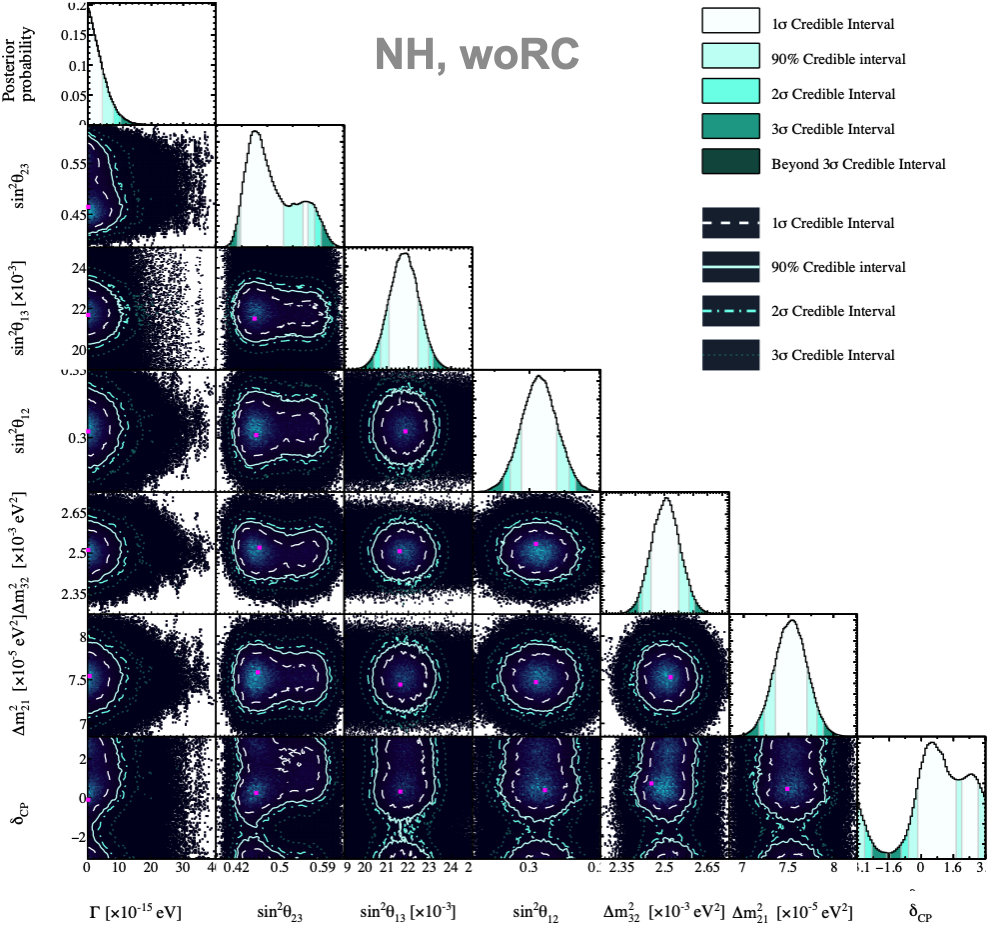
\includegraphics[width=1.\textwidth]{figures/TrianglePlots/T2K_B4/T2K_B4_QD_asimov_woRC_trianglePlot_nh.png}
    %{figures/TrianglePlots/T2K_B4/QD_asimov_woRC_trianglePlot_bothMH.pdf}
	\caption[Quantum Decoherence and Neutrino Oscillation Parameter Posterior Distributions of T2K B marginalised over the \acrlong{nh} without Reactor Constraint with Zero Decoherence Strength.]{The $1$- (upper plots) and $2$-dimensional posterior distributions of the oscillation parameters and decoherence strength from the T2K accelerator-neutrino fit marginalised over the \acrfull{nh}. The $1\sigma$ (white, dashed), $90\%$ (light cyan, solid), $2\sigma$ (dark cyan, dotted-dashed), $3\sigma$ (green, dotted) and beyond $3\sigma$ (dark green) credible regions in the $1$-dimensional distributions are shown with the same colours in the $2$-dimensional contours. The Asimov point in this fit is $\left[ \sin^2(\theta_{12}), \sin^2(\theta_{23}), \sin^2(\theta_{13}), \Delta m^2_{12}, \Delta m^2_{23}, \delta_\text{CP}, \Gamma \right] =$ $\left[ 0.307, 0.450, 0.022, 7.53 \times 10{-3}, 2.494 \times 10^{-3}, 0.0, 0.0 \right]$ (\textit{T2K Set B with zero decoherence strength}). The reactor constraint is not applied (woRC).}
	\label{fig:T2K_B4/QD_asimov_woRC_trianglePlot_nh}
    \end{figure}
%

%
    \begin{figure}[hbt]
	\centering
	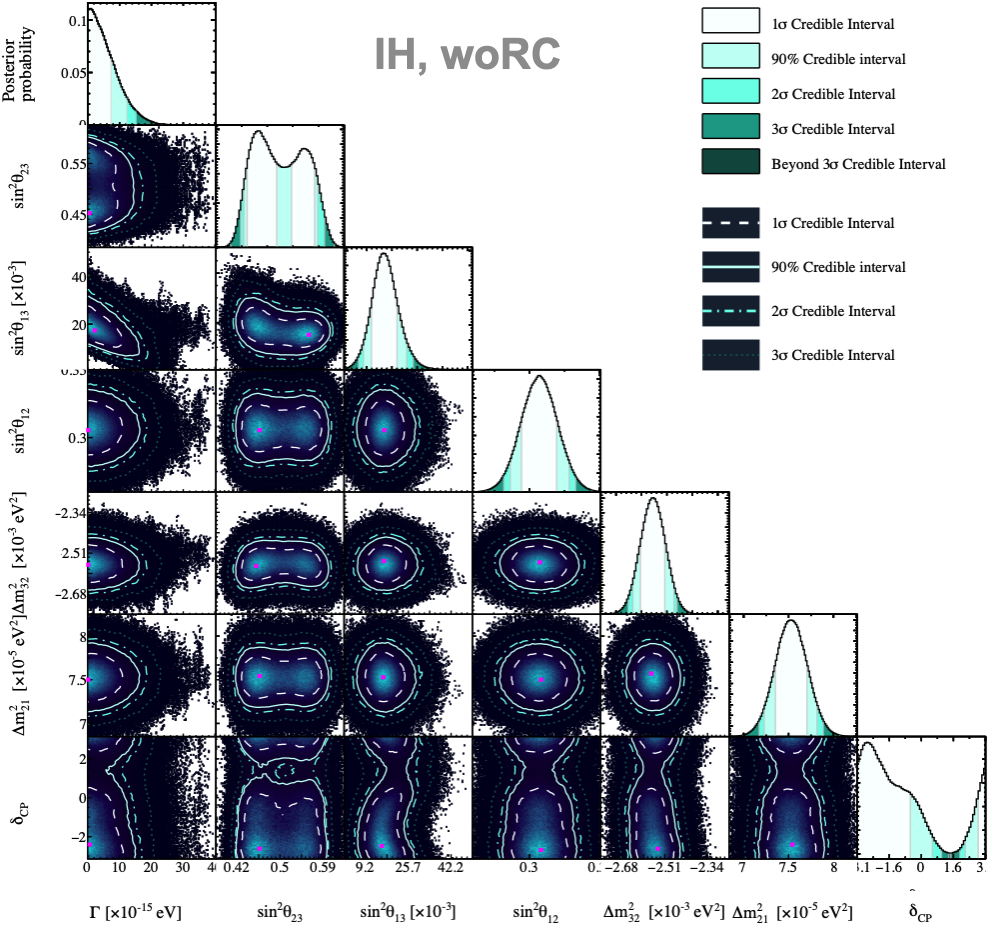
\includegraphics[width=1.\textwidth]{figures/TrianglePlots/T2K_B4/T2K_B4_QD_asimov_woRC_trianglePlot_ih.png}
    %{figures/TrianglePlots/T2K_B4/QD_asimov_woRC_trianglePlot_bothMH.pdf}
	\caption[Quantum Decoherence and Neutrino Oscillation Parameter Posterior Distributions of T2K B marginalised over the \acrlong{ih} without Reactor Constraint with Zero Decoherence Strength.]{The $1$- (upper plots) and $2$-dimensional posterior distributions of the oscillation parameters and decoherence strength from the T2K accelerator-neutrino fit marginalised over the \acrfull{ih}. The $1\sigma$ (white, dashed), $90\%$ (light cyan, solid), $2\sigma$ (dark cyan, dotted-dashed), $3\sigma$ (green, dotted) and beyond $3\sigma$ (dark green) credible regions in the $1$-dimensional distributions are shown with the same colours in the $2$-dimensional contours. The Asimov point in this fit is $\left[ \sin^2(\theta_{12}), \sin^2(\theta_{23}), \sin^2(\theta_{13}), \Delta m^2_{12}, \Delta m^2_{23}, \delta_\text{CP}, \Gamma \right] =$ $\left[ 0.307, 0.450, 0.022, 7.53 \times 10{-3}, 2.494 \times 10^{-3}, 0.0, 0.0 \right]$ (\textit{T2K Set B with zero decoherence strength}). The reactor constraint is not applied (woRC).}
	\label{fig:T2K_B4/QD_asimov_woRC_trianglePlot_ih}
    \end{figure}
%

%
    \begin{figure}[hbt]
	\centering
	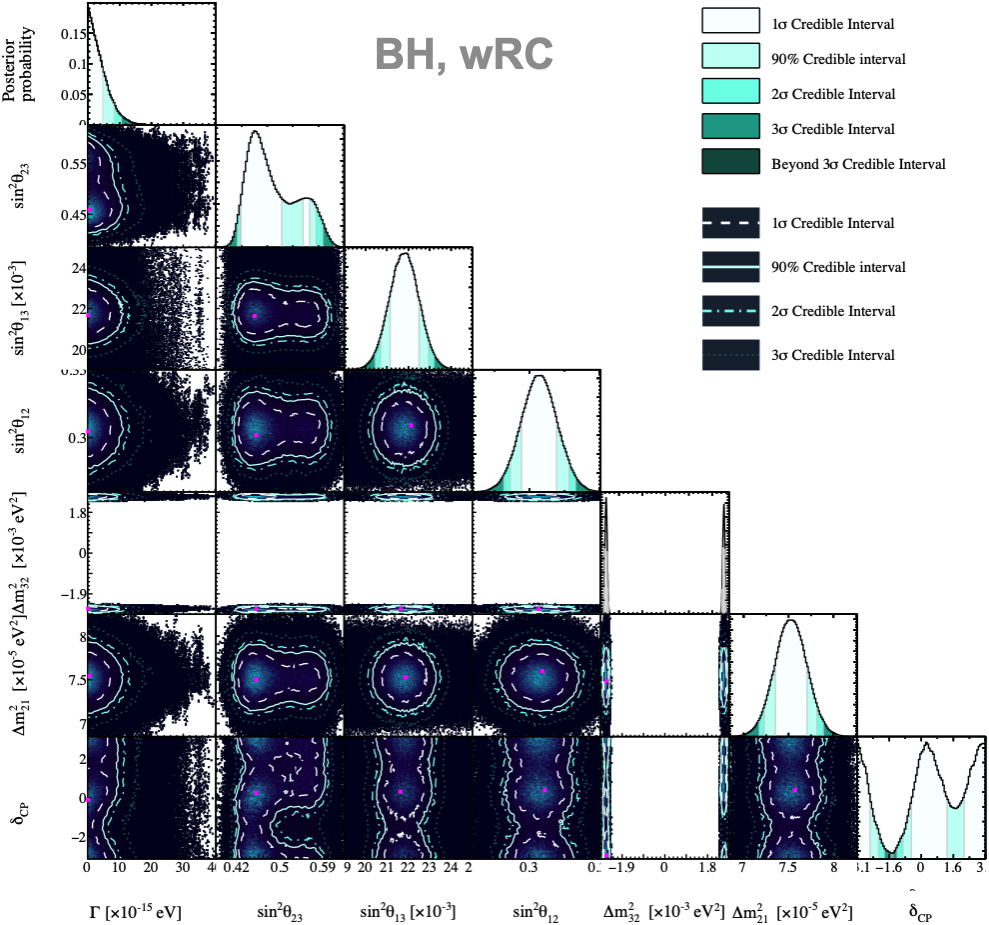
\includegraphics[width=1.\textwidth]{figures/TrianglePlots/T2K_B4/T2K_B4_QD_asimov_wRC_trianglePlot_bothMH.png}
    %{figures/TrianglePlots/T2K_B4/QD_asimov_woRC_trianglePlot_bothMH.pdf}
	\caption[Quantum Decoherence and Neutrino Oscillation Parameter Posterior Distributions of T2K B marginalised over \acrlong{bh} with Reactor Constraint with Zero Decoherence Strength.]{The $1$- (upper plots) and $2$-dimensional posterior distributions of the oscillation parameters and decoherence strength from the T2K accelerator-neutrino fit marginalised over \acrfull{bh}. The $1\sigma$ (white, dashed), $90\%$ (light cyan, solid), $2\sigma$ (dark cyan, dotted-dashed), $3\sigma$ (green, dotted) and beyond $3\sigma$ (dark green) credible regions in the $1$-dimensional distributions are shown with the same colours in the $2$-dimensional contours. The Asimov point in this fit is $\left[ \sin^2(\theta_{12}), \sin^2(\theta_{23}), \sin^2(\theta_{13}), \Delta m^2_{12}, \Delta m^2_{23}, \delta_\text{CP}, \Gamma \right] =$ $\left[ 0.307, 0.450, 0.022, 7.53 \times 10{-3}, 2.494 \times 10^{-3}, 0.0, 0.0 \right]$ (\textit{T2K Set B with zero decoherence strength}). The reactor constraint is applied (wRC).}
	\label{fig:T2K_B4/QD_asimov_wRC_trianglePlot_bothMH}
    \end{figure}
%

%
    \begin{figure}[hbt]
	\centering
	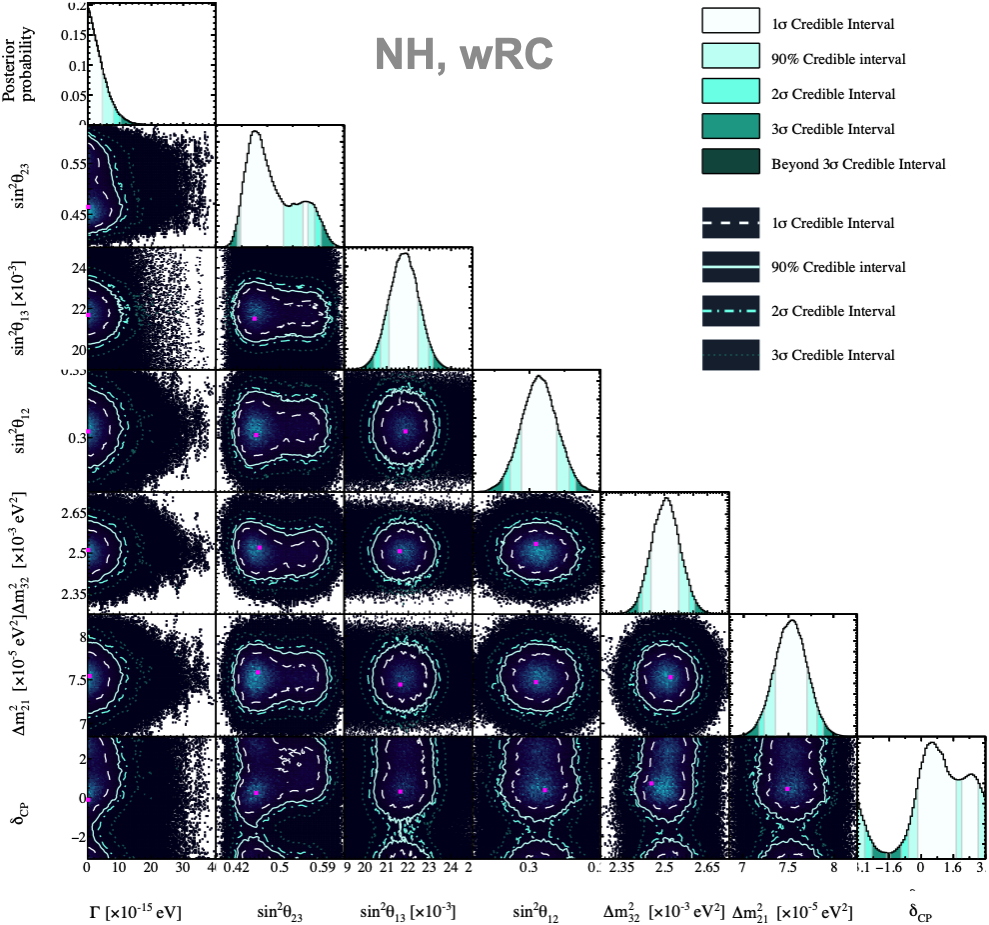
\includegraphics[width=1.\textwidth]{figures/TrianglePlots/T2K_B4/T2K_B4_QD_asimov_wRC_trianglePlot_nh.png}
    %{figures/TrianglePlots/T2K_B4/QD_asimov_woRC_trianglePlot_bothMH.pdf}
	\caption[Quantum Decoherence and Neutrino Oscillation Parameter Posterior Distributions of T2K B marginalised over the \acrlong{nh} with Reactor Constraint with Zero Decoherence Strength.]{The $1$- (upper plots) and $2$-dimensional posterior distributions of the oscillation parameters and decoherence strength from the T2K accelerator-neutrino fit marginalised over the \acrfull{nh}. The $1\sigma$ (white, dashed), $90\%$ (light cyan, solid), $2\sigma$ (dark cyan, dotted-dashed), $3\sigma$ (green, dotted) and beyond $3\sigma$ (dark green) credible regions in the $1$-dimensional distributions are shown with the same colours in the $2$-dimensional contours. The Asimov point in this fit is $\left[ \sin^2(\theta_{12}), \sin^2(\theta_{23}), \sin^2(\theta_{13}), \Delta m^2_{12}, \Delta m^2_{23}, \delta_\text{CP}, \Gamma \right] =$ $\left[ 0.307, 0.450, 0.022, 7.53 \times 10{-3}, 2.494 \times 10^{-3}, 0.0, 0.0 \right]$ (\textit{T2K Set B with zero decoherence strength}). The reactor constraint is applied (wRC).}
	\label{fig:T2K_B4/QD_asimov_wRC_trianglePlot_nh}
    \end{figure}
%

%
    \begin{figure}[hbt]
	\centering
	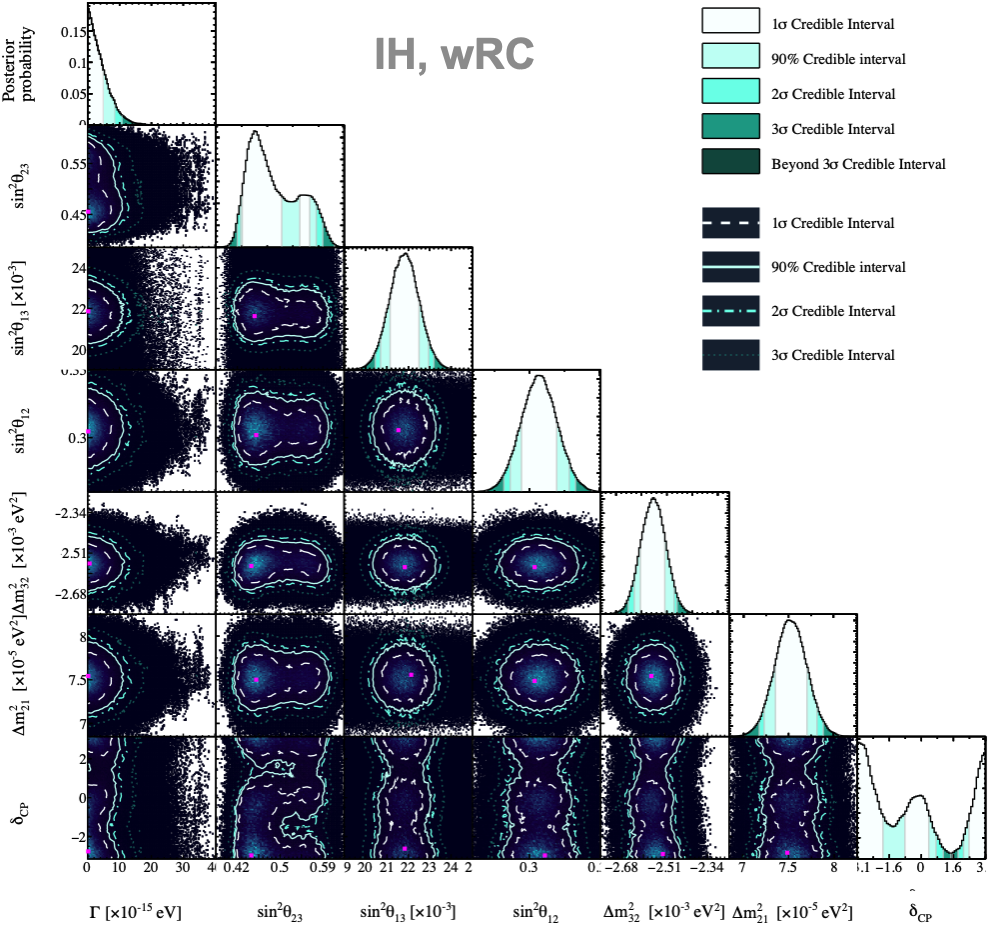
\includegraphics[width=1.\textwidth]{figures/TrianglePlots/T2K_B4/T2K_B4_QD_asimov_wRC_trianglePlot_ih.png}
    %{figures/TrianglePlots/T2K_B4/QD_asimov_woRC_trianglePlot_bothMH.pdf}
	\caption[Quantum Decoherence and Neutrino Oscillation Parameter Posterior Distributions of T2K B marginalised over the \acrlong{ih} with Reactor Constraint with Zero Decoherence Strength.]{The $1$- (upper plots) and $2$-dimensional posterior distributions of the oscillation parameters and decoherence strength from the T2K accelerator-neutrino fit marginalised over the \acrfull{ih}. The $1\sigma$ (white, dashed), $90\%$ (light cyan, solid), $2\sigma$ (dark cyan, dotted-dashed), $3\sigma$ (green, dotted) and beyond $3\sigma$ (dark green) credible regions in the $1$-dimensional distributions are shown with the same colours in the $2$-dimensional contours. The Asimov point in this fit is $\left[ \sin^2(\theta_{12}), \sin^2(\theta_{23}), \sin^2(\theta_{13}), \Delta m^2_{12}, \Delta m^2_{23}, \delta_\text{CP}, \Gamma \right] =$ $\left[ 0.307, 0.450, 0.022, 7.53 \times 10{-3}, 2.494 \times 10^{-3}, 0.0, 0.0 \right]$ (\textit{T2K Set B with zero decoherence strength}). The reactor constraint is applied (wRC).}
	\label{fig:T2K_B4/QD_asimov_wRC_trianglePlot_ih}
    \end{figure}
%

%
    \begin{figure}[hbt]
	\centering
	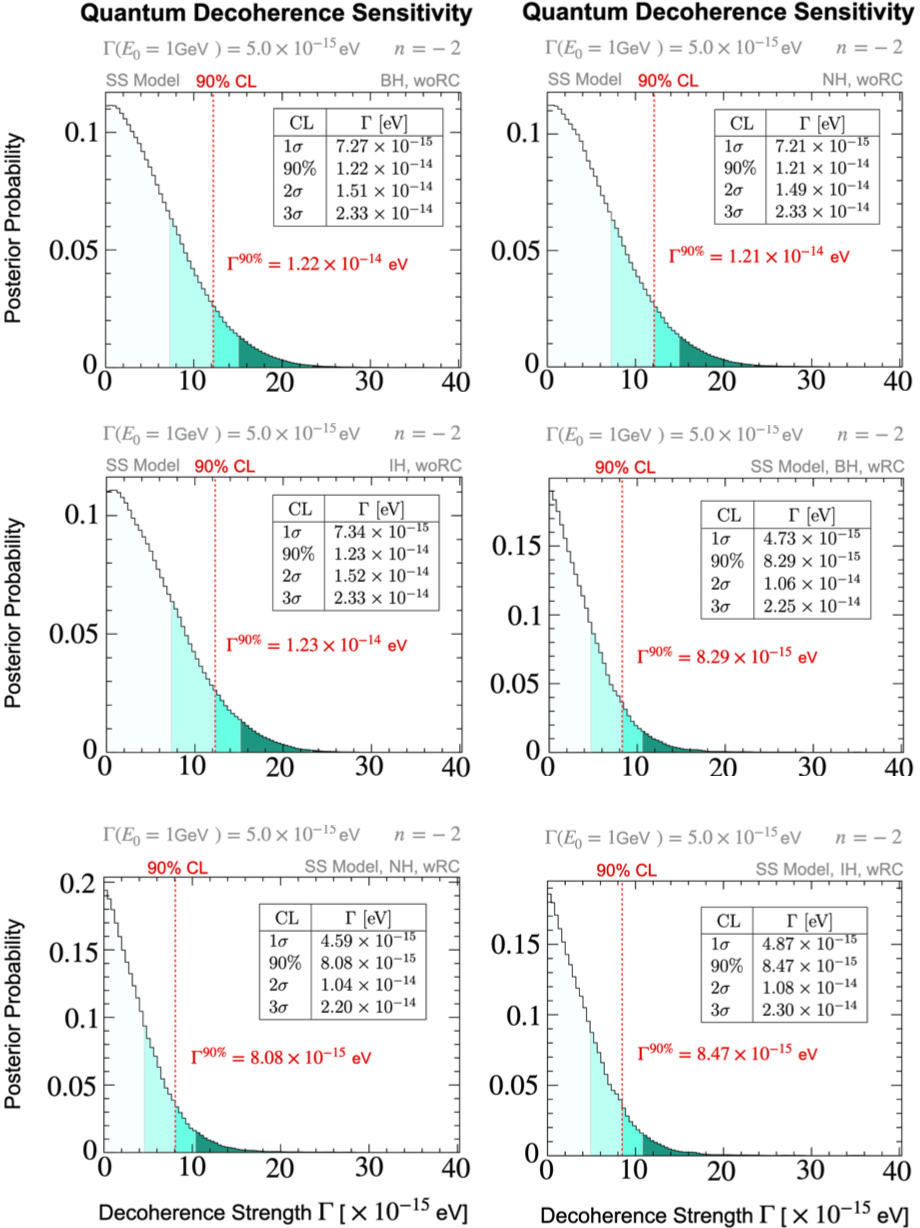
\includegraphics[width=1.\textwidth]{figures/TrianglePlots/T2K_B4/T2K_B4_QD_asimov_1d_decostrength_cis2.png}
    %{figures/TrianglePlots/T2K_B4/T2K_B4_QD_asimov_1d_decostrength_cis.png}
	\caption[Quantum Decoherence Posterior Distributions of T2K B with Zero Decoherence Strength.]{Quantum decoherence posterior distributions of T2K B with zero decoherence strength as displayed in figs. \ref{fig:T2K_B4/QD_asimov_woRC_trianglePlot_bothMH}-\ref{fig:T2K_B4/QD_asimov_wRC_trianglePlot_ih}.}
    \label{fig:T2K_B4/T2K_B4_QD_asimov_1d_decostrength_cis}
    \end{figure}
%




\iffalse
%
    \begin{figure}[hbt]
	\centering
	\includegraphics[width=1.\textwidth]%{figures/TrianglePlots/T2K_A1/QD_asimov_woRC_trianglePlot_nh.pdf}
	\caption{The $1$- (upper plots) and $2$-dimensional posterior distributions of the oscillation parameters and decoherence strength from the T2K accelerator-neutrino fit for the normal hierarchy. The $1\sigma$ (white, dashed), $90\%$ (light cyan, solid), $2\sigma$ (dark cyan, dotted-dashed), $3\sigma$ (green, dotted) and beyond $3\sigma$ (dark green) credible regions in the $1$-dimensional distributions are shown with the same colours in the $2$-dimensional contours. The Asimov point in this fit is $\left[ \sin^2(\theta_{12}), \sin^2(\theta_{23}), \sin^2(\theta_{13}), \Delta m^2_{12}, \Delta m^2_{23}, \delta_\text{CP}, \Gamma \right] =$ $\left[ 0.307, 0.561, 0.022, 7.53 \times 10{-3}, 2.494 \times 10^{-3}, -1.601, 5.0 \times 10 {-15} \right]$ (\textit{T2K Set A with non-zero decoherence strength}). The reactor constraint is not applied (woRC).}
	\label{fig:T2K_A1/QD_asimov_woRC_trianglePlot_nh}
    \end{figure}
%

%
    \begin{figure}[hbt]
	\centering
	\includegraphics[width=1.\textwidth]%{figures/TrianglePlots/T2K_A1/QD_asimov_woRC_trianglePlot_nh.pdf}
	\caption{The $1$- (upper plots) and $2$-dimensional posterior distributions of the oscillation parameters and decoherence strength from the T2K accelerator-neutrino fit for the normal hierarchy. The $1\sigma$ (white, dashed), $90\%$ (light cyan, solid), $2\sigma$ (dark cyan, dotted-dashed), $3\sigma$ (green, dotted) and beyond $3\sigma$ (dark green) credible regions in the $1$-dimensional distributions are shown with the same colours in the $2$-dimensional contours. The Asimov point in this fit is $\left[ \sin^2(\theta_{12}), \sin^2(\theta_{23}), \sin^2(\theta_{13}), \Delta m^2_{12}, \Delta m^2_{23}, \delta_\text{CP}, \Gamma \right] =$ $\left[ 0.307, 0.561, 0.022, 7.53 \times 10{-3}, 2.494 \times 10^{-3}, -1.601, 5.0 \times 10 {-15} \right]$ (\textit{T2K Set A with non-zero decoherence strength}). The reactor constraint is not applied (woRC).}
	\label{fig:T2K_A1/QD_asimov_woRC_trianglePlot_nh}
    \end{figure}
%
\fi